\chapter{Results\label{cha:results}}
This chapter presents the results of various experiments of the proposed concept including evaluation of how effective the representations from different language models are for anomaly detection on 1) already seen log data during training and 2) unstable log data that changes due to log updates. In particular, the language models Bert, XL-Transformers and GPT-2, as described in \ref{sec:word_vectorization}, are compared. Additionally, the regression-based method, described in \ref{sec:regression}, and the classification method, described in \ref{sec:classification}, are compared, showing advantages or disadvantages among each other.

Section \ref{sec:experimental_setup} lists details about the used hardware and technologies, followed by section \ref{sec:evaluation}, in which the results of the evaluation are presented. Finally, section \ref{sec:discussion_results} presents the results of the evaluation.


\section{Experimental Setup\label{sec:experimental_setup}}
In this section, the used hardware, libraries and the dimensions of the word embeddings for every language model and the used log dataset are described.

\subsection{Hardware and Library Specifications}
The machine that was used to conduct the experiments has the following specifications:
\begin{itemize}
	\item Intel(R) Core(TM) i5-9600K CPU @ 3.70GHz
	\item 128 GB RAM
	\item 2 x NVIDIA GeForce RTX 2080 Ti 11GB RAM
	\item Ubuntu 18.04.3 LTS
\end{itemize}

\noindent The most relevant libraries that were used are:
\begin{itemize}
	\item Python 3.6.7
	\item Numpy 1.14.5
	\item PyTorch 1.4.0
	\item Transformers 2.3.0
	\item Tensorflow 2.1.0
\end{itemize}

\noindent The word embedding vector of the used language models have the following dimensions:
\begin{itemize}
	\item Bert: 768 
	\item GPT-2: 768
	\item XL-Transformers: 1024
\end{itemize}

\subsection{Anomaly Detection on one Dataset \label{sec:ad_one_ds_result}}
For evaluating the model the OpenStack datasets ``normal log dataset 2" (referenced to as original dataset from now on) containing 137k log lines and the ``log dataset having performance anomalies" containing 18k log lines (referenced to as test dataset from now on), provided by Loghub, are utilised \cite{utah_dataset}. The original dataset stems from logs  that were recorded by running multiple OpenStack instances for 20 hours and 13 minutes on CloudLab \cite{cloudlab}, and 2 hours and 17 minutes for the test dataset. 

The test dataset contains anomalies which are only detectable by inspecting the parameters of the log events, as described in \ref{fig:parsing}, i.e. the variable part of the log event which is not visible in the template after parsing. Therefore, a total of 5\% of anomalies in relation to the total number of lines of the test dataset are injected into the test dataset, yielding a labeled test dataset for evaluation of the trained model. This is necessary due to the assumptions specified in \ref{sec:requirements_and_assumptions}. Two types of anomalies are injected separately:
\begin{enumerate}
	\item An anomaly that is \textit{semantically different} from the other log events. In this case the log event ``\textit{Timeout for executing the request}" is injected at a ratio of 5\%. In order to assess the quality of the used word embeddings further, log alterations are additionally injected into the dataset containing anomalies, in order to simulate the instability of logs as described in \ref{sec:logs_alteration}.
	\item Anomalies that are \textit{semantically similar} to the other log events. For 5\% of the log lines, 50\% of the words are replaced by other words (e.g. ``time", ``during", ``causing", ``replace" and ``crashed"). For example, ``\textit{Took seconds to build instance}" will be changed to ``\textit{Took \textcolor{red}{replace} \textcolor{red}{during} build \textcolor{red}{causing}}".
\end{enumerate}
Table \ref{tab:test_train_ds} gives an overview of the amount of log lines per dataset. The number of \textit{raw lines} reflects the number of log lines in the dataset's initial state, while the number of \textit{lines ordered} specifies the number of log lines after the log has been ordered by instance id, as described in \ref{sec:conceptlogparsing} and depicted in \ref{fig:full_preprocessing_pipeline}.


\begin{table}[ht]
\centering
\begin{small}
\begin{tabular}{ p{1.3cm} p{1.8cm} p{2.3cm} p{1.7cm}}
\toprule
Dataset & \#lines raw & \#lines ordered & Anomalies\\
\midrule
Train & 137k & 33k & 0\%\\
Test & 18k & 5k & 5\%\\ 

\bottomrule
\end{tabular}
\caption{Test and train dataset.}
\label{tab:test_train_ds}
\end{small}
\end{table}



\subsection{Transfer of Knowledge \label{sec:transfer_learning_setup}}
In order to examine the ability of the model to transfer the knowledge obtained from one dataset to a different one, the same OpenStack log dataset utilised in \ref{sec:ad_one_ds_result} is used as a basis. For this experiment, all occurrences of the templates which are visible in figure \ref{fig:transfer_modifications} on the left side are replaced by the templates visible on the right side. Additionally, all alterations presented in section \ref{sec:logs_alteration} - line shuffling, duplication and deletion; and word insertion, removal and replacement - are injected into the dataset at ratios of 5\%, 10\% and 15\% each in dataset $A$. This heavy modifications simulate a different version of the dataset. Then, the model is trained on this dataset $A$ for 60 epochs. Dataset $B$, the unaltered version of dataset $A$ is then used to conduct few-shot training on the model, followed by anomaly detection on a dataset that has the same characteristics as dataset $B$, i.e. no alterations.

\begin{figure}[H]
  \centering
  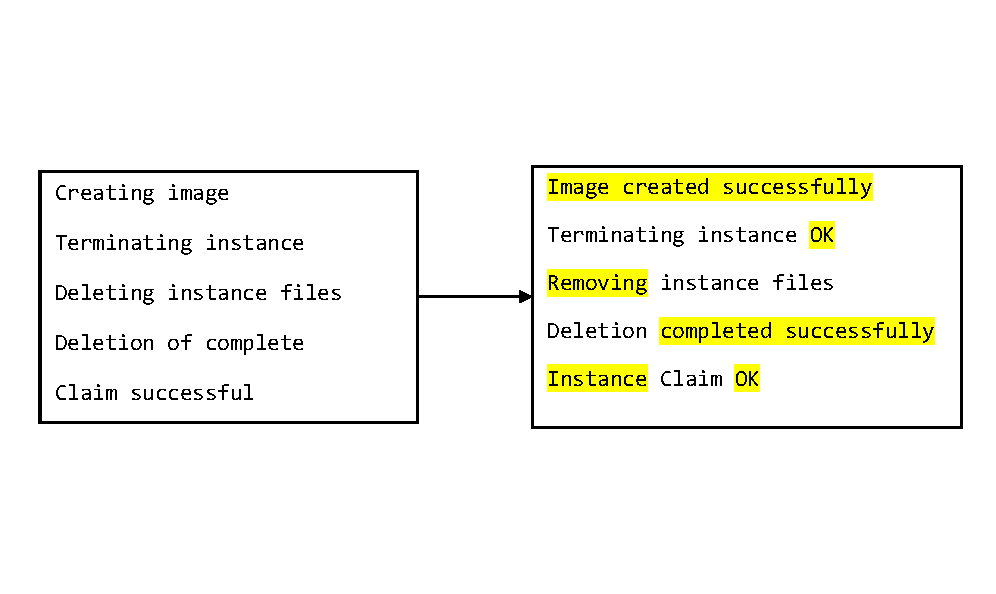
\includegraphics[width=11cm]{transfer_modifications.pdf}\\
  \caption{Changes on templates of the original dataset.}
  \label{fig:transfer_modifications}
\end{figure}




\section{Evaluation\label{sec:evaluation}}
In this section the results of the evaluation between the two anomaly detection approaches, the regression-based approach and the classification-based approach are compared using three different language models: namely Bert, XL-Transformers and GPT-2. The pre-processing steps string cleansing and finetuning, as described in \ref{sec:pre_processing}, are investigated with regards to their potential on benefiting the quality of the word embeddings. Subsequently, the results of the evaluation using one dataset and the transfer of knowledge approach are presented.

\subsection{String cleansing}
String cleansing, as described in \ref{sec:template_cleansing}, can potentially improve the distinguishability between templates drastically in the used dataset.
For Bert a heatmap that shows the pairwise cosine distances between templates before cleansing is depicted in figure \ref{fig:bert_before_cleansing}. The corresponding distances after cleansing in figure \ref{fig:bert_after_cleansing}. The corresponding templates for the indices on the x and y axes before and after cleansing can be found in table \ref{tab:templates_before_cleansing} and table \ref{tab:templates_after_cleansing}, respectively.
The cosine distances before and after cleansing for GPT-2 can be found in figure \ref{fig:gpt_before_cleansing} and figure \ref{fig:gpt_after_cleansing}, and for XL-Transformer in figure \ref{fig:xl_before_cleansing} and figure \ref{fig:xl_after_cleansing}, respectively. The average pairwise cosine distances between templates before and after cleansing can be seen in table \ref{tab:average_pairwise_cos_distances}.
The average cosine distance between templates increases by 96\% for GPT-2, yet the initial value is already very low with only 0.0027. We can see how the average cosine distance between templates increases for Bert by 84\%, from 0.2718 to 0.5004 and for XL-Transformers from 0.2511 to 0.7001. While Bert has a slightly higher average pairwise cosine distance before cleansing, XL-Transformers highly benefits from cleansing demonstrated by an increase of 178\%. This underlines the importance of this step in order to meet the requirements postulated in \ref{sec:word_vectorization}, depending on the utilised language models.



\begin{table}[ht]
\centering
\begin{small}
\begin{tabular}{ p{1.3cm} p{2.5cm} p{2.5cm} }
\toprule
Model & Before cleansing & After cleansing\\
\midrule
XL & 0.2511 & 0.7001\\
Bert & 0.2718 & 0.5004\\
GPT-2 & 0.0027 & 0.0053 \\ 

\bottomrule
\end{tabular}
\caption{Average pairwise template cosine distances.}
\label{tab:average_pairwise_cos_distances}
\end{small}
\end{table}


\begin{figure}[!tbp]
  \centering
  \subfloat[Before cleansing.]{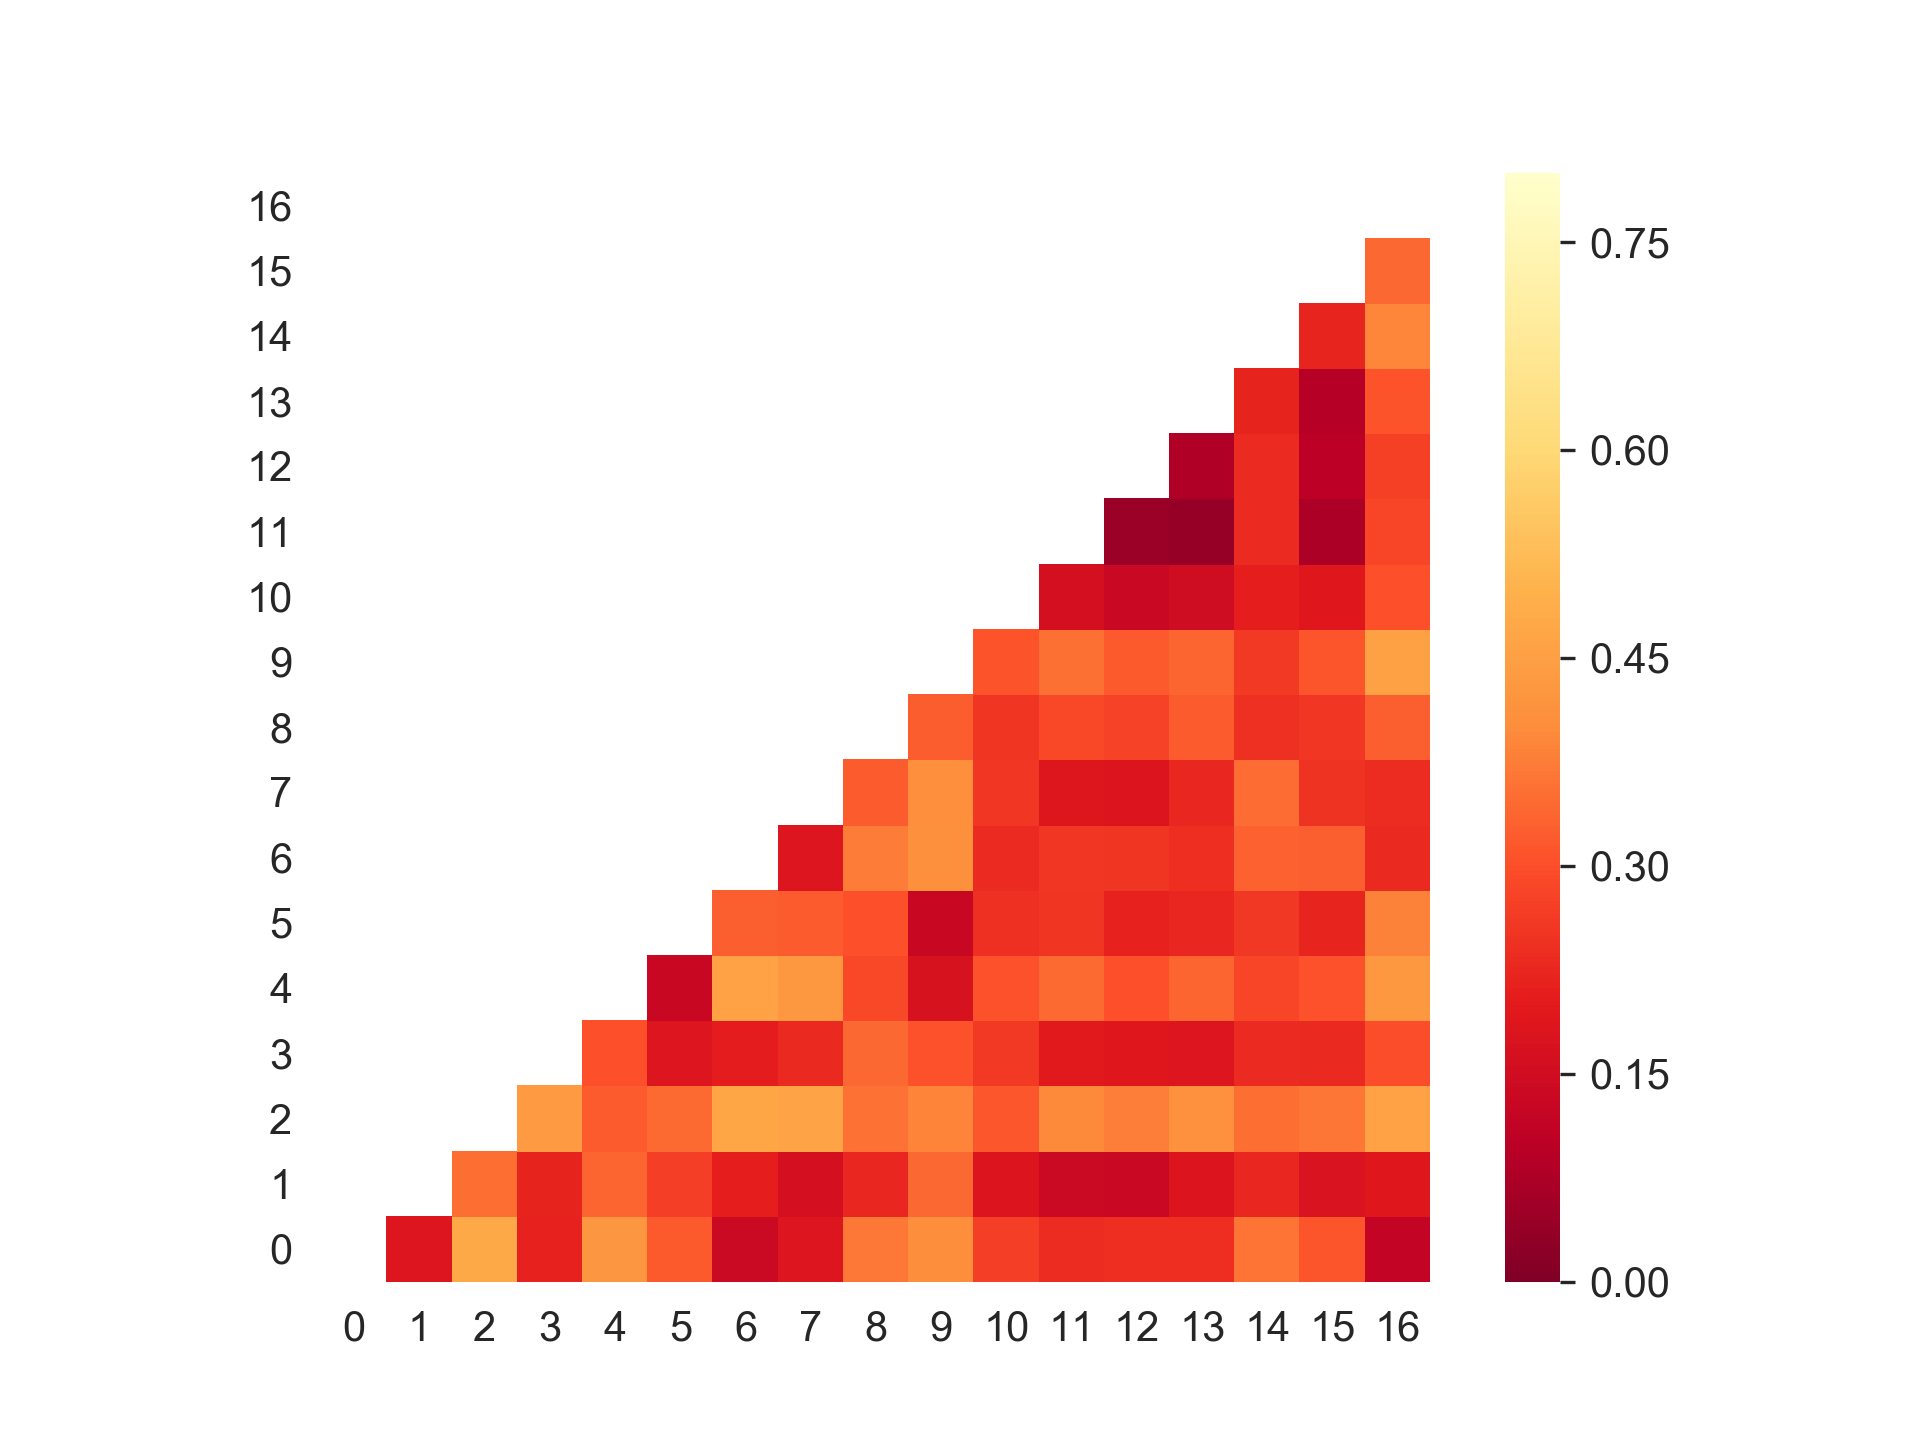
\includegraphics[width=0.48\textwidth]{bert_before_cleansing.png}\label{fig:bert_before_cleansing}}
  \hfill
  \subfloat[After cleansing.]{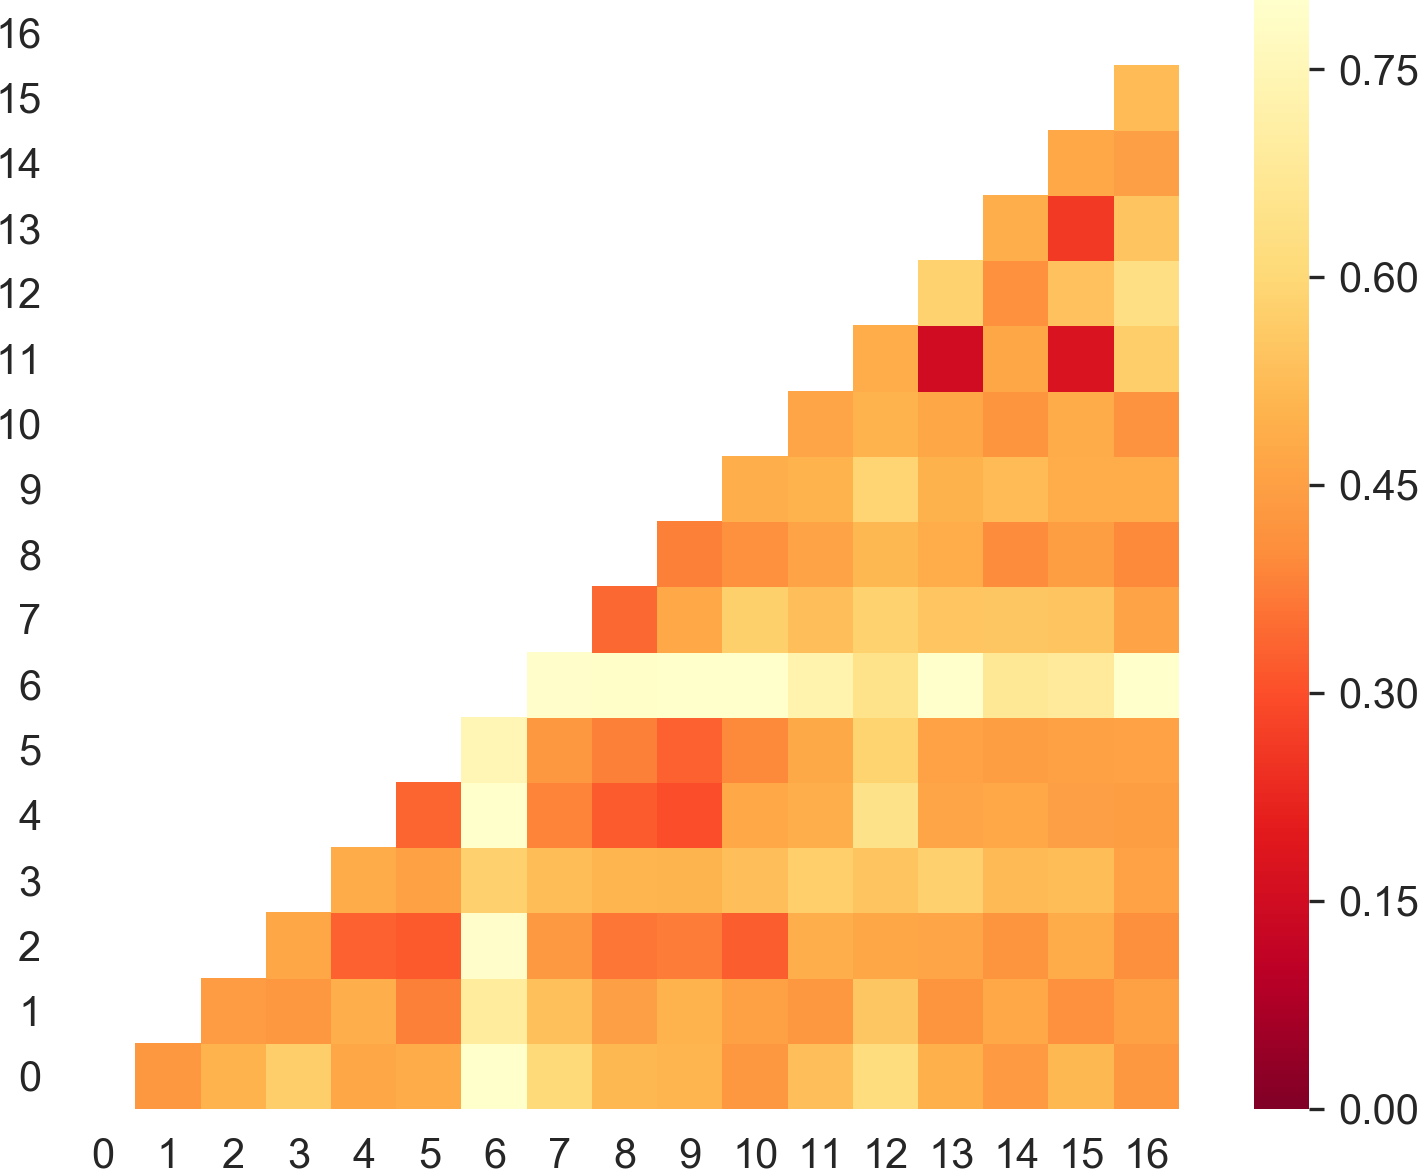
\includegraphics[width=0.48\textwidth]{bert_after_cleansing.png}\label{fig:bert_after_cleansing}}
  \caption{Bert pairwise template cosine distance.}
\end{figure}

\begin{figure}[!tbp]
  \centering
  \subfloat[Before cleansing.]{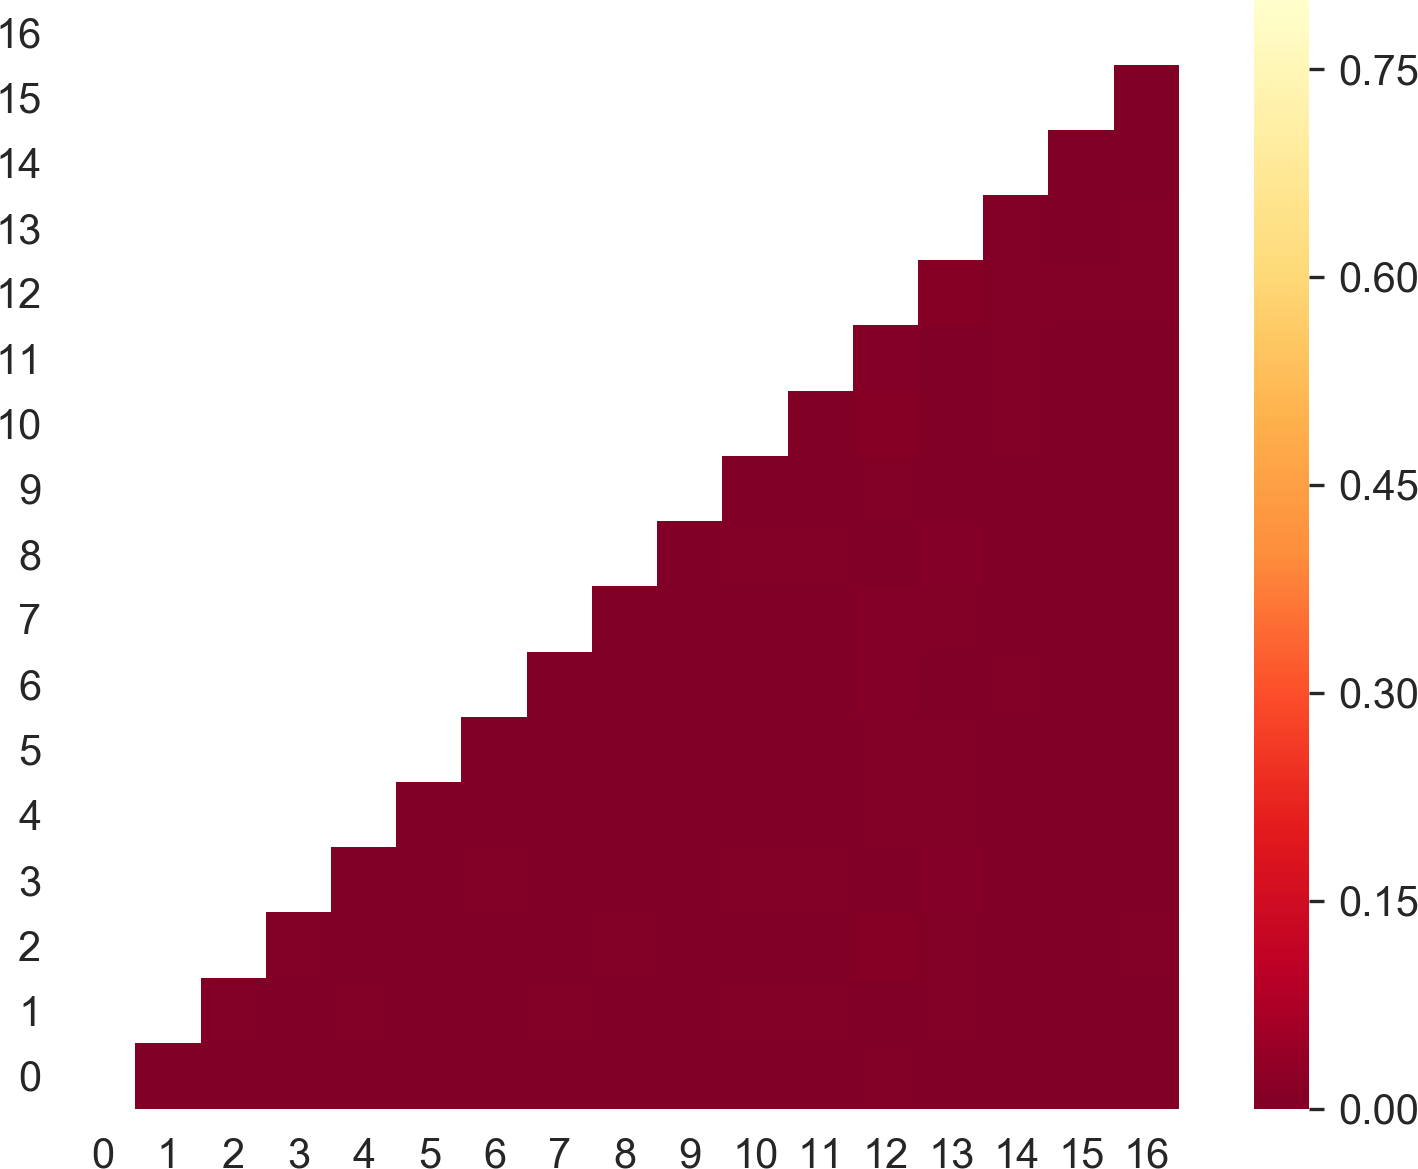
\includegraphics[width=0.48\textwidth]{gpt_before_cleansing.png}\label{fig:gpt_before_cleansing}}
  \hfill
  \subfloat[After cleansing.]{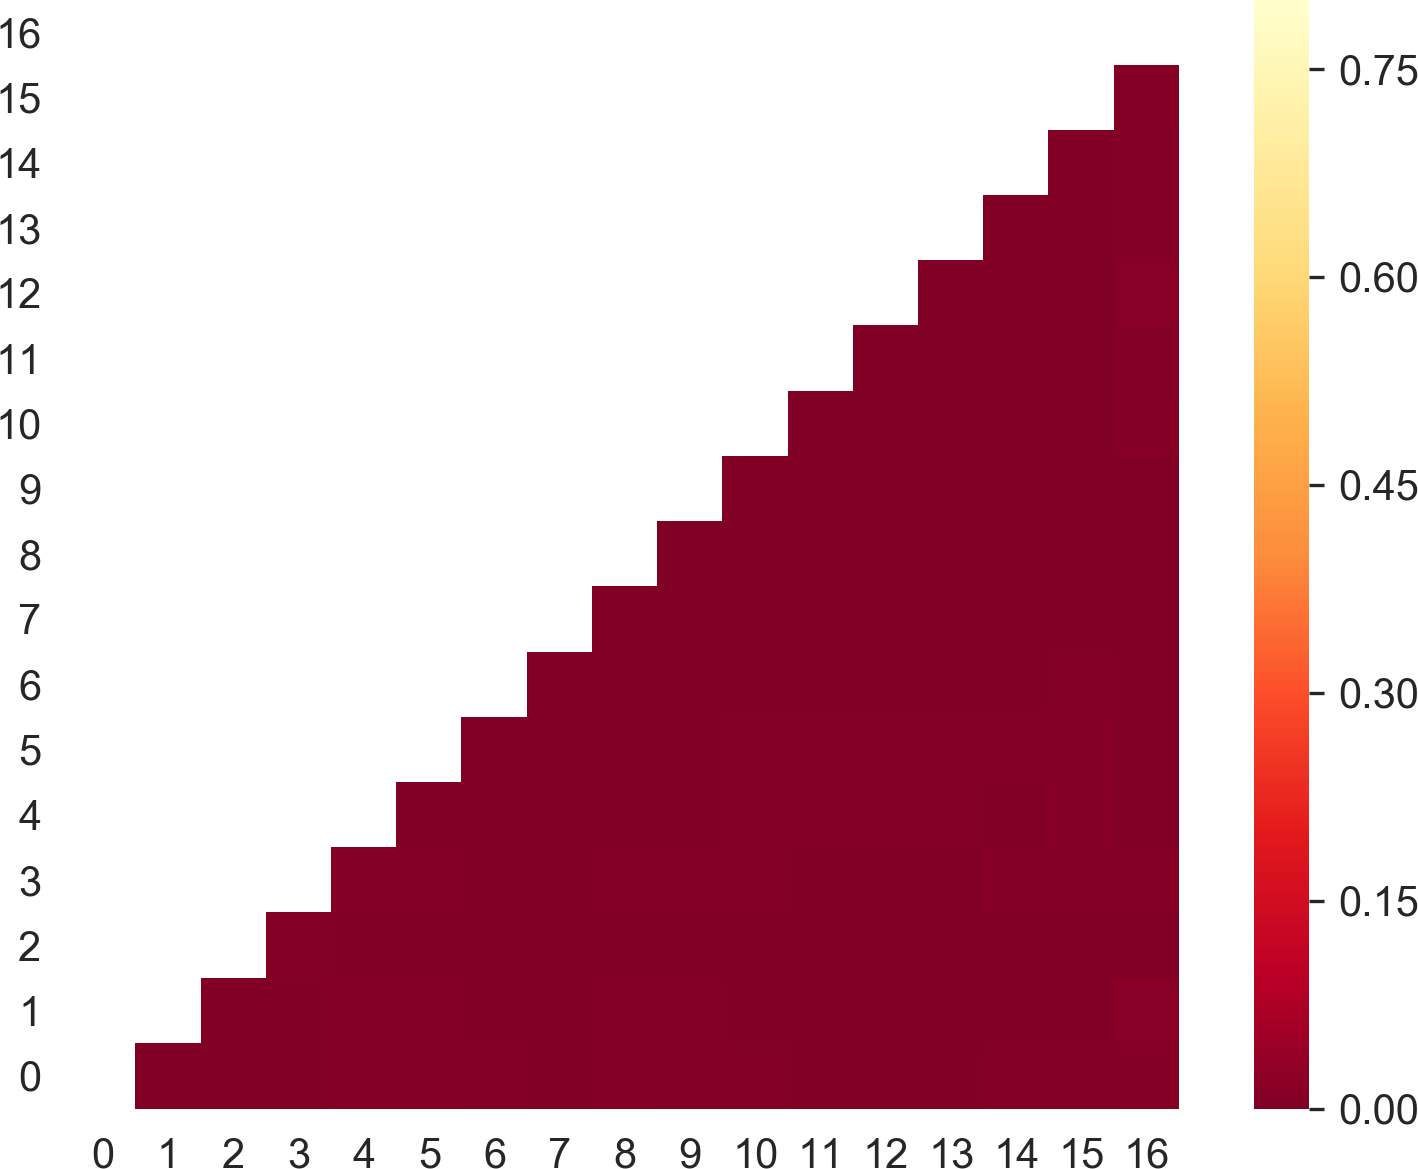
\includegraphics[width=0.48\textwidth]{gpt_after_cleansing.png}\label{fig:gpt_after_cleansing}}
  \caption{GPT-2 pairwise template cosine distance.}
\end{figure}

\begin{figure}[!tbp]
  \centering
  \subfloat[Before cleansing.]{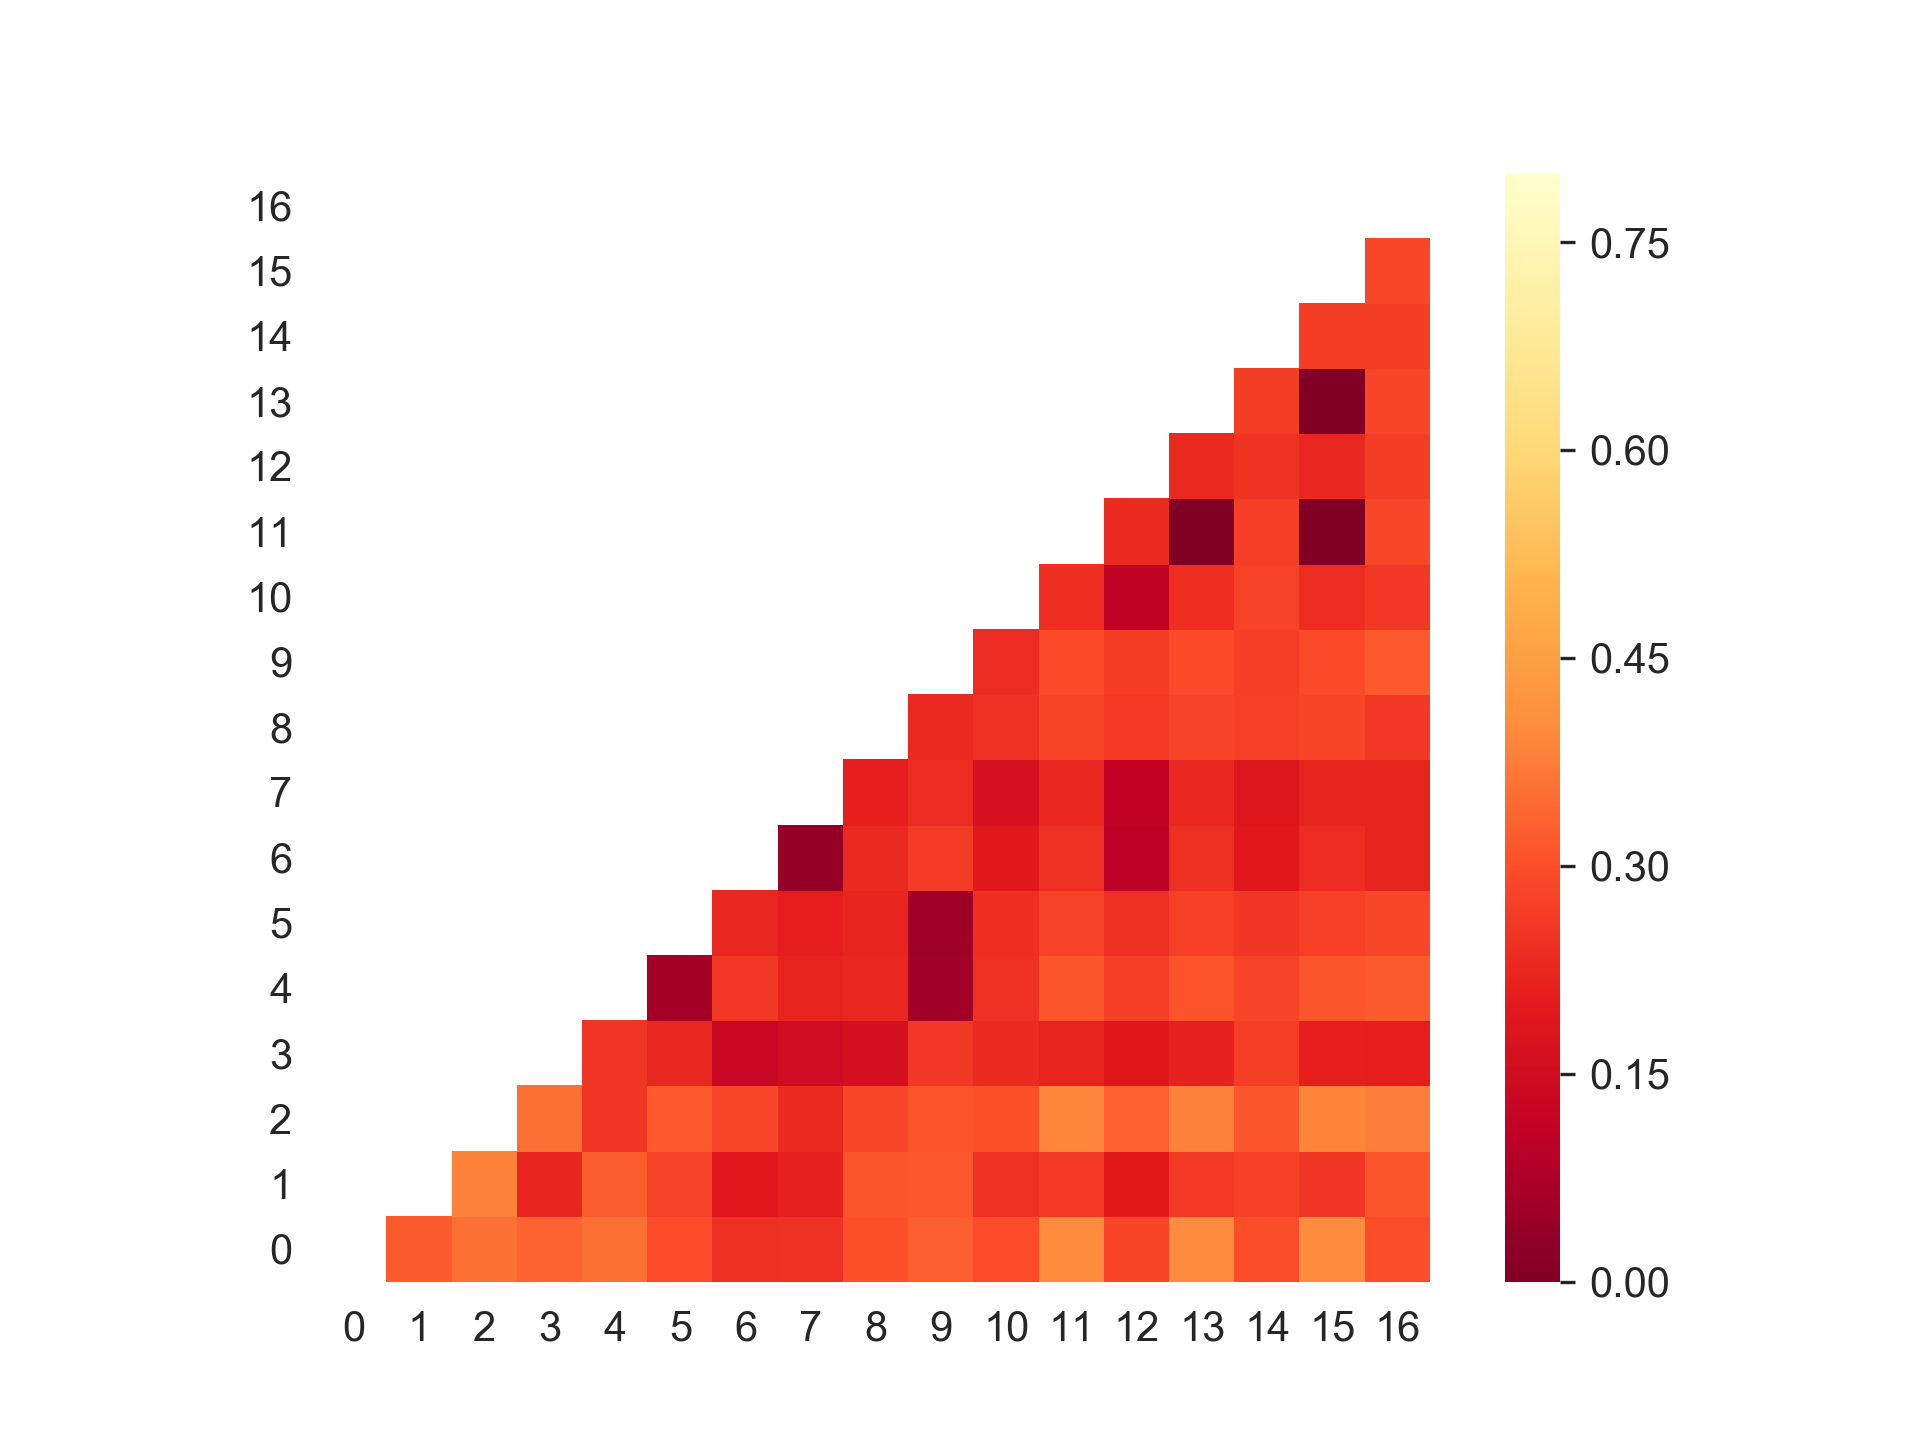
\includegraphics[width=0.48\textwidth]{xl_before_cleansing.png}\label{fig:xl_before_cleansing}}
  \hfill
  \subfloat[After cleansing.]{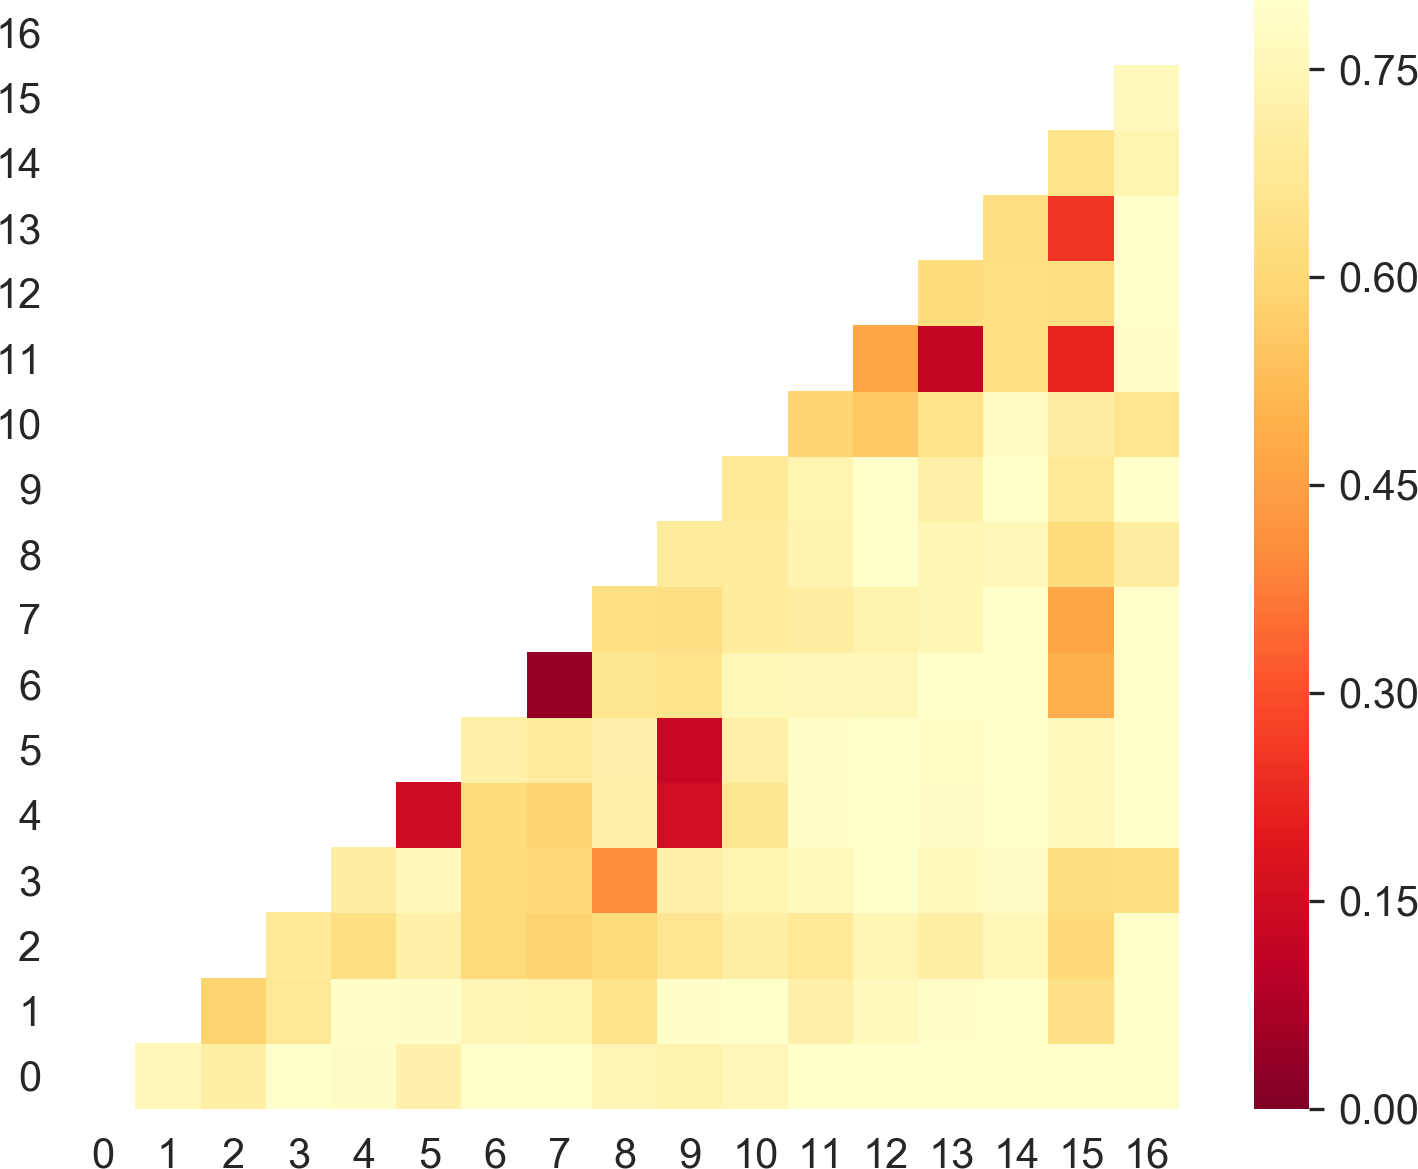
\includegraphics[width=0.48\textwidth]{xl_after_cleansing.png}\label{fig:xl_after_cleansing}}
  \caption{XL-Transformers pairwise template cosine distance.}
\end{figure}




\begin{table}[ht]
\begin{small}
\centering
\begin{tabular}{ c l } 
\toprule
Index & Template \\
\midrule
0 & $\langle*\rangle$ Creating image\\
1 & $\langle*\rangle$ VM $\langle*\rangle$ (Lifecycle Event)\\
2 & $\langle*\rangle$ During sync\_power\_state the instance has a pending task (spawning). Skip.\\
3 & $\langle*\rangle$ Instance $\langle*\rangle$ successfully.\\
4 & $\langle*\rangle$ Took $\langle*\rangle$.$\langle*\rangle$ seconds to $\langle*\rangle$ the instance on the hypervisor.\\
5 & $\langle*\rangle$ Took $\langle*\rangle$.$\langle*\rangle$ seconds to build instance.\\
6 & $\langle*\rangle$ Terminating instance\\
7 & $\langle*\rangle$ Deleting instance files $\langle*\rangle$\\
8 & $\langle*\rangle$ Deletion of $\langle*\rangle$ complete\\
9 & $\langle*\rangle$ Took $\langle*\rangle$.$\langle*\rangle$ seconds to deallocate network for instance.\\
10 & $\langle*\rangle$ Attempting claim: memory $\langle*\rangle$ MB, disk $\langle*\rangle$ GB, vcpus $\langle*\rangle$ CPU\\
11 & $\langle*\rangle$ Total memory: $\langle*\rangle$ MB, used: $\langle*\rangle$.$\langle*\rangle$ MB\\
12 & $\langle*\rangle$ memory limit: $\langle*\rangle$.$\langle*\rangle$ MB, free: $\langle*\rangle$.$\langle*\rangle$ MB\\
13 & $\langle*\rangle$ Total disk: $\langle*\rangle$ GB, used: $\langle*\rangle$.$\langle*\rangle$ GB\\
14 & $\langle*\rangle$ $\langle*\rangle$ limit not specified, defaulting to unlimited\\
15 & $\langle*\rangle$ Total vcpu: $\langle*\rangle$ VCPU, used: $\langle*\rangle$.$\langle*\rangle$ VCPU\\
16 & $\langle*\rangle$ Claim successful\\
\bottomrule
\end{tabular}
\caption{Templates before cleansing.}
\label{tab:templates_before_cleansing}
\end{small}
\end{table}



\begin{table}[ht]
\begin{small}
\centering
\begin{tabular}{ c l } 
\toprule
Index & Template \\
\midrule
0 & Creating image\\
1 & VM  Lifecycle Event\\
2 & During sync power state the instance has a pending task spawning Skip\\
3 & Instance  successfully\\
4 & Took  seconds to  the instance on the hypervisor\\
5 & Took  seconds to build instance\\
6 & Terminating instance\\
7 & Deleting instance files\\
8 & Deletion of complete\\
9 & Took  seconds to deallocate network for instance\\
10 & Attempting claim memory  MB disk  GB vcpus  CPU\\
11 & Total memory  MB used  MB\\
12 & memory limit  MB free  MB\\
13 & Total disk  GB used  GB\\
14 & limit not specified defaulting to unlimited\\
15 & Total vcpu  VCPU used  VCPU\\
16 & Claim successful\\
\bottomrule
\end{tabular}
\caption{Templates after cleansing.}
\label{tab:templates_after_cleansing}
\end{small}
\end{table}

\clearpage
\subsection{Finetuning}
As described in \ref{sec:finetuning}, finetuning can potentially help producing word embeddings that are more adequate for solving certain natural language processing tasks. As described in \ref{sec:word_vectorization}, a high cosine distance between semantically different templates is required. The dataset that consists of the templates in table \ref{tab:templates_after_cleansing} has been chosen for finetuning. Since the pre-trained language models Bert, GPT-2 an XL-Transformers have been trained on a large corpus, finetuning would also need to be executed on a sufficiently large corpus. Since this is not the case, the results of finetuning for a maximum of four epochs, as suggested by the Bert authors \cite{devlin2018bert}, does not yield the desired results. As it can be seen in figure \ref{fig:cos_distance_finetuning}, it was not possible to increase the cosine distances between templates on the task of Masked LM (as described in \ref{Bert}), compared to the cosine distances depicted in figure \ref{fig:bert_after_cleansing}. The average distance between templates dropped from 0.4449 to 0.3016. The fact that the loss on the evaluation part of the dataset is not decreasing adequately, as shown in figure \ref{fig:finetuning_loss}, shows that through learning on such a small corpus it is not possible to generalise well enough, which makes finetuning on the default learning task not useful in this case. Since the Huggingface Transformers library does not offer finetuning interfaces for GPT-2 and XL-Transformers on the same task as for Bert, they are not further investigated for finetuning.

\begin{figure}[H]
  \centering
  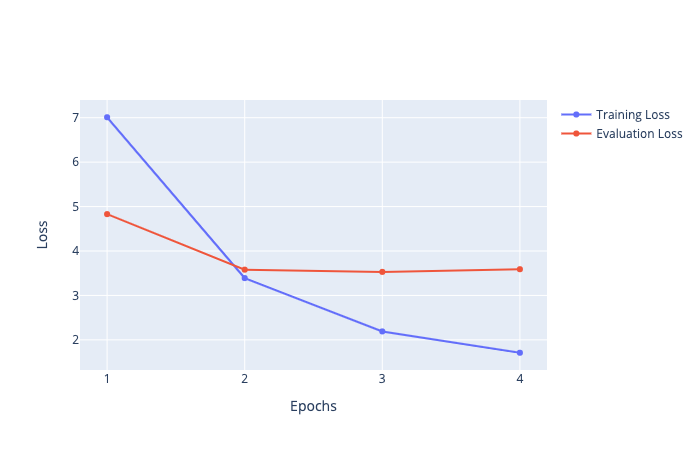
\includegraphics[width=9cm,height=6.7cm]{finetuning_loss.png}\\
  \caption{Training and evaluation loss for finetuning on masked LM.}
  \label{fig:finetuning_loss}
\end{figure}

\clearpage
\begin{figure}[h]
  \centering
  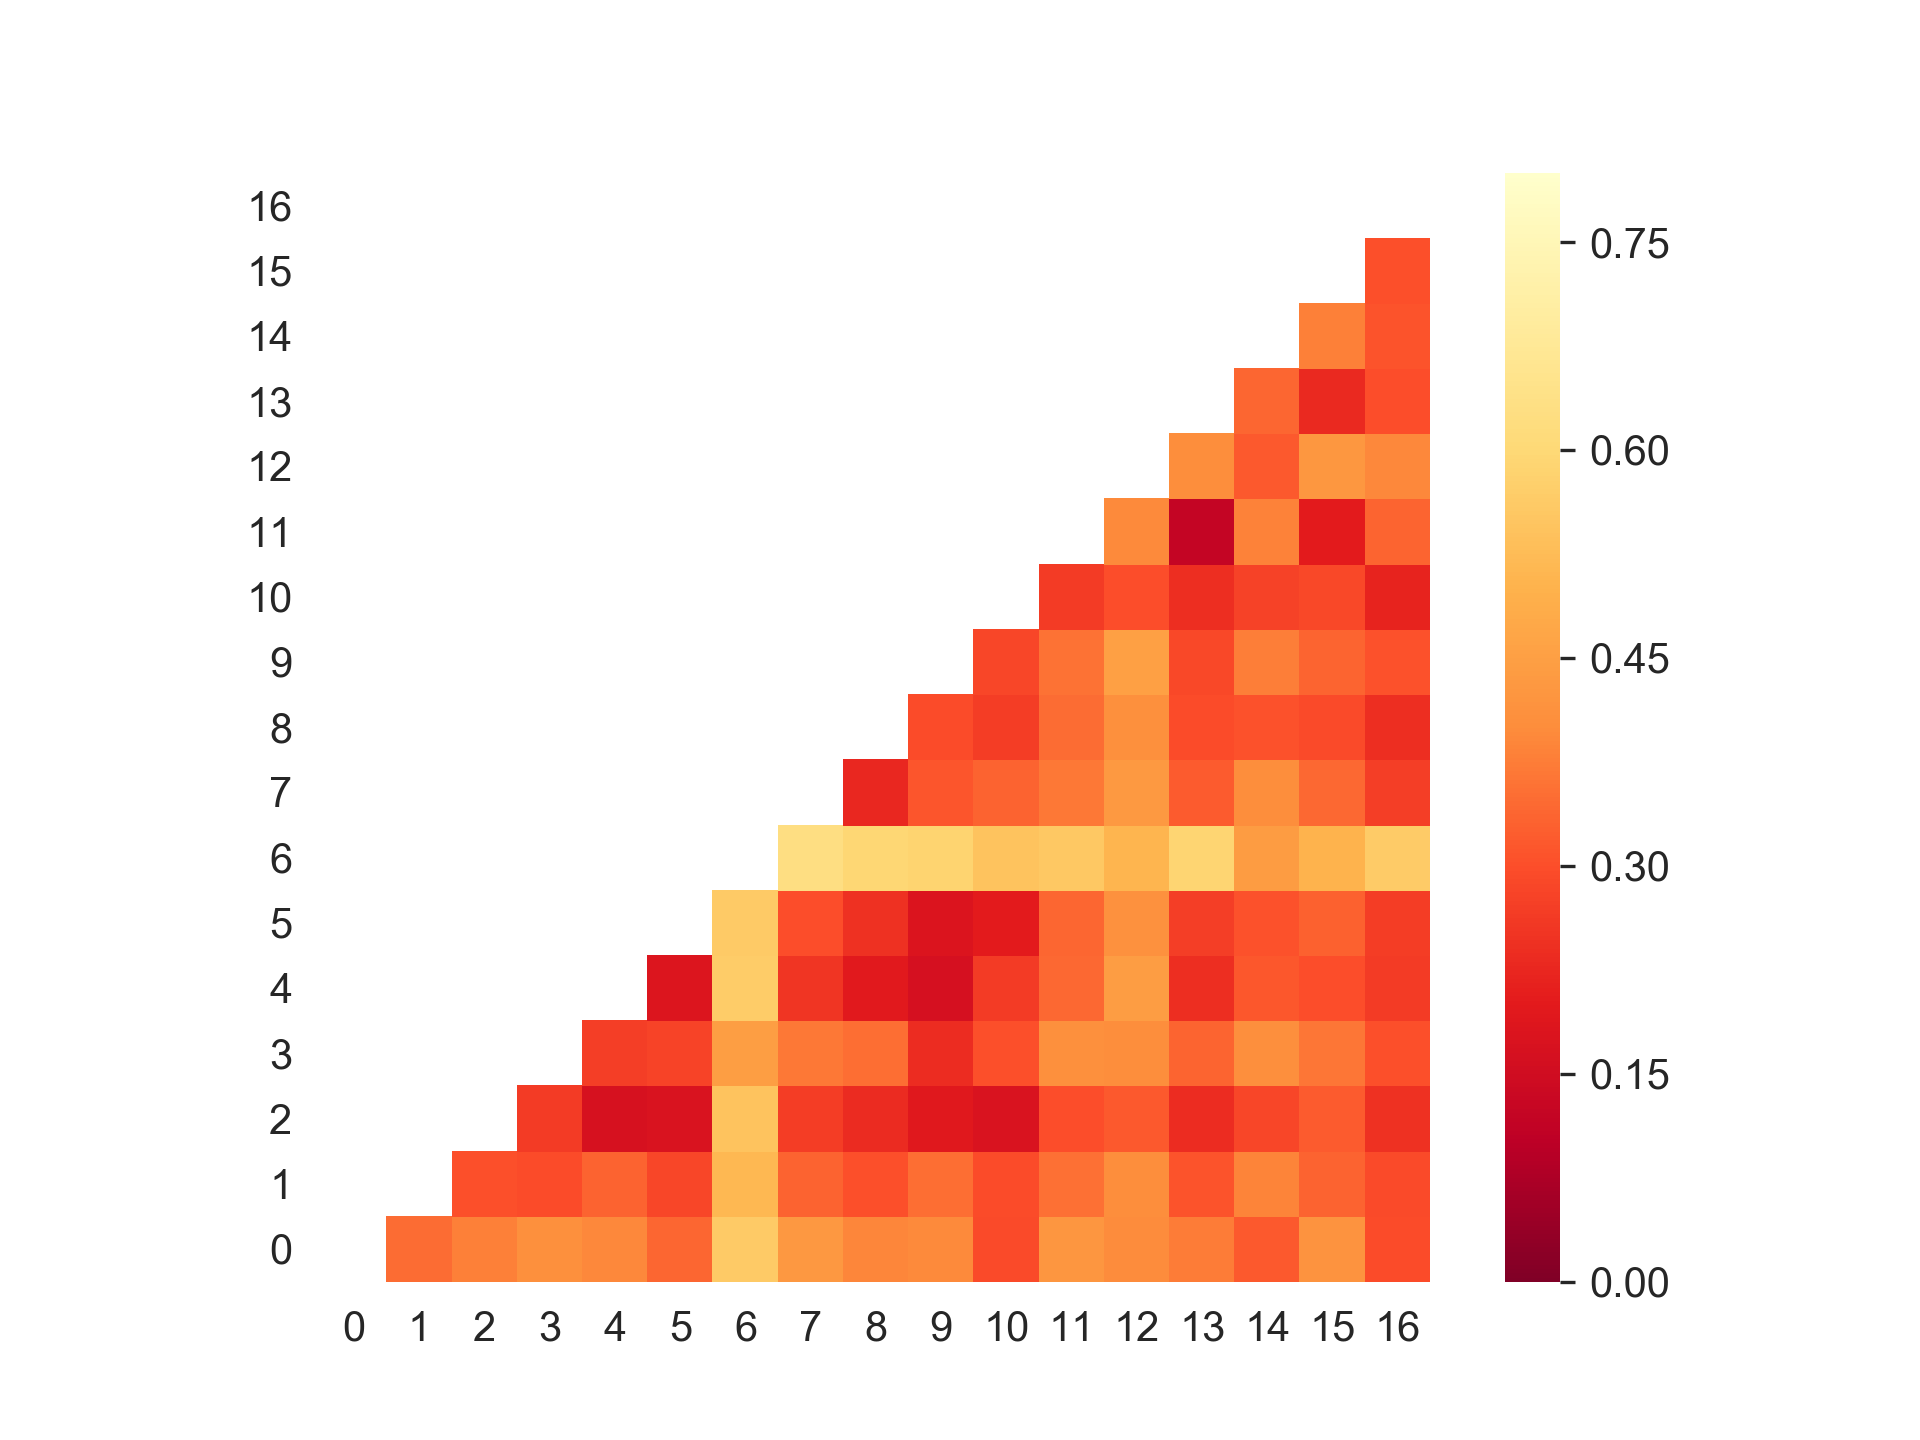
\includegraphics[width=12cm,height=9cm]{bert_finetuning_cleansed.png}\\
  \caption{Cosine distance between templates after cleansing and finetuning}
  \label{fig:cos_distance_finetuning}
\end{figure}


\subsection{Hyperparameters}
In order to find well-suited parameters for the LSTM model, it was initially applied to the problem using a minimal configuration. With the help of a grid-search and running simulations with different configurations, the following hyperparameters have proven to yield the most satisfying results:
\begin{itemize}
	\item 512 hidden units for the bidirectional LSTM, with one layer;
	\item two fully connected layers with 512 units $\rightarrow$ 256 units and 256 units $\rightarrow$ output size;
	\item dropout of 0.1 between every layer;
	\item input sequence length of 7;
	\item 60 epochs of training.
\end{itemize}

%%%%%%%%%%%%
% REGRESSION 
%%%%%%%%%%%%
\subsection{Regression\label{sec:results-regression}}
In this subsection the results of the regression-based approach, including various alterations using the three different language models, are presented. In order to evaluate the robustness of the language models to the evolution and instability of log events, alterations as described in \ref{sec:logs_alteration} are injected at different ratios. The impact on detecting semantically different anomalies after alterations on the sequence of logs are injected, i.e. deleting, shuffling and duplicating events are summarised in figure \ref{fig:results_regression_sequential}. Alterations are not injected all at the same time, but independently from each other. The results in the figures are average values of all experiments with alterations on the log sequences. Results broken down by each alteration can be found in the appendix \ref{appendix:regression}. From 5\% to 15\% alterations, both Bert and GPT-2 show recall values of 1.0, while XL-Transformers is only able to detect 61\% to 65\% of all anomalies. With regards to precision, GPT-2 achieves values from 0.91 for 5\% alterations to 1.0 for 10\% alterations to 0.88 for 15\% alterations, while Bert declines from 0.55 at 5\% alterations to 0.43 with 15\% alterations. XL-Transformers in turn returns low values of 0.32 for 5\% alterations to 0.21 for 15\% alterations. Moreover, for F1-score GPT-2 achieves very good results with about 0.95 for all alteration ratios, while Bert declines from 0.69 for 5\% alterations to 0.56 for 15\% alterations. XL-Transformers achieves a F1-score of 0.42 for 5\% alterations, 0.34 for 10\% alterations and 0.31 for 15\% alterations. It is evident that GPT-2 performs better than Bert and XL-Transformers in all metrics in this category, except for recall, where Bert is performing equally well. Bert can be located as second place in this category, while XL-Transformers delivers the least promising results in comparison to Bert and GPT-2.

In addition to the alterations on the log sequences, alterations on the log events themselves, i.e. inserting, removing and replacing words are also of interest, with subsequent injection of semantically different anomalies. The results of this experiment can be seen in figure \ref{fig:results_regression_words}. Again, the alterations are not injected all at once, but independently -- the figure shows averaged results. Exactly as for the previous results, we can see that both Bert and GPT-2 achieve a recall value of 1.0 for all alteration ratios, while XL-Transformers achieves results of around 0.63 for all alteration ratios. GPT-2 performs equally good on both F1-score and precision as in the previous experiments, while Bert achieves F1-scores which are between 8 and 10 percentage points better, and for precision improvements of around 7 percentage points. XL-Transformers shows even higher improvements than Bert, with an average improvement of 13 percentage points for F1-score and an average improvement of 17 percentage points for precision, with a slight degradation in recall of 3 percentage points on average. Again, GPT-2 shows the best results overall, followed by Bert and XL-Transformers.

The results for injecting semantically similar anomalies can be see in figure \ref{fig:replace_words_regression}. It is clearly visible that this experiment shows a different picture than the previous ones. GPT-2 achieves less qualitative results than before, while Bert and especially XL-Transformers show partly better results than they did with the the injection of semantically different anomalies. Bert achieves a F1-score of 0.71, XL-Transformers 0.6 and GPT-2 0.09. Also with regards to precision the results are slightly better for Bert and XL-Transformers - Bert achieving 0.61, XL-Transformers 0.6, but GPT-2 only 0.13. XL-Transformers shows improvements for recall with 0.75, while Bert degrades to 0.86 and GPT-2 degrades to 0.07. This experiment, complementary to the previous ones, where a semantically different anomaly line was injected and GPT-2 proved to be robust, shows that GPT-2 is not able to detect semantically similar anomalies well. Bert is most useful for the task of anomaly detection using the regression approach overall.

Another aspect that is evaluated is the impact of the input sequence length, i.e. the number of concatenated log events, for which the next log event shall be predicted on the ability of the model to detect anomalies. The results of this evaluation can be seen in \ref{fig:seq_len_regression}, where for 15\% of the log lines one random word is inserted as alteration, and 5\% semantically different anomalies are injected. Bert profits from sequence lengths longer or equal to 6, whereas the quality of results for GPT-2 and XL-Transformers are not as affected from the input sequence length, but are generally lower for XL-Transformers.

\begin{comment}
\begin{figure}[h]
  \centering
  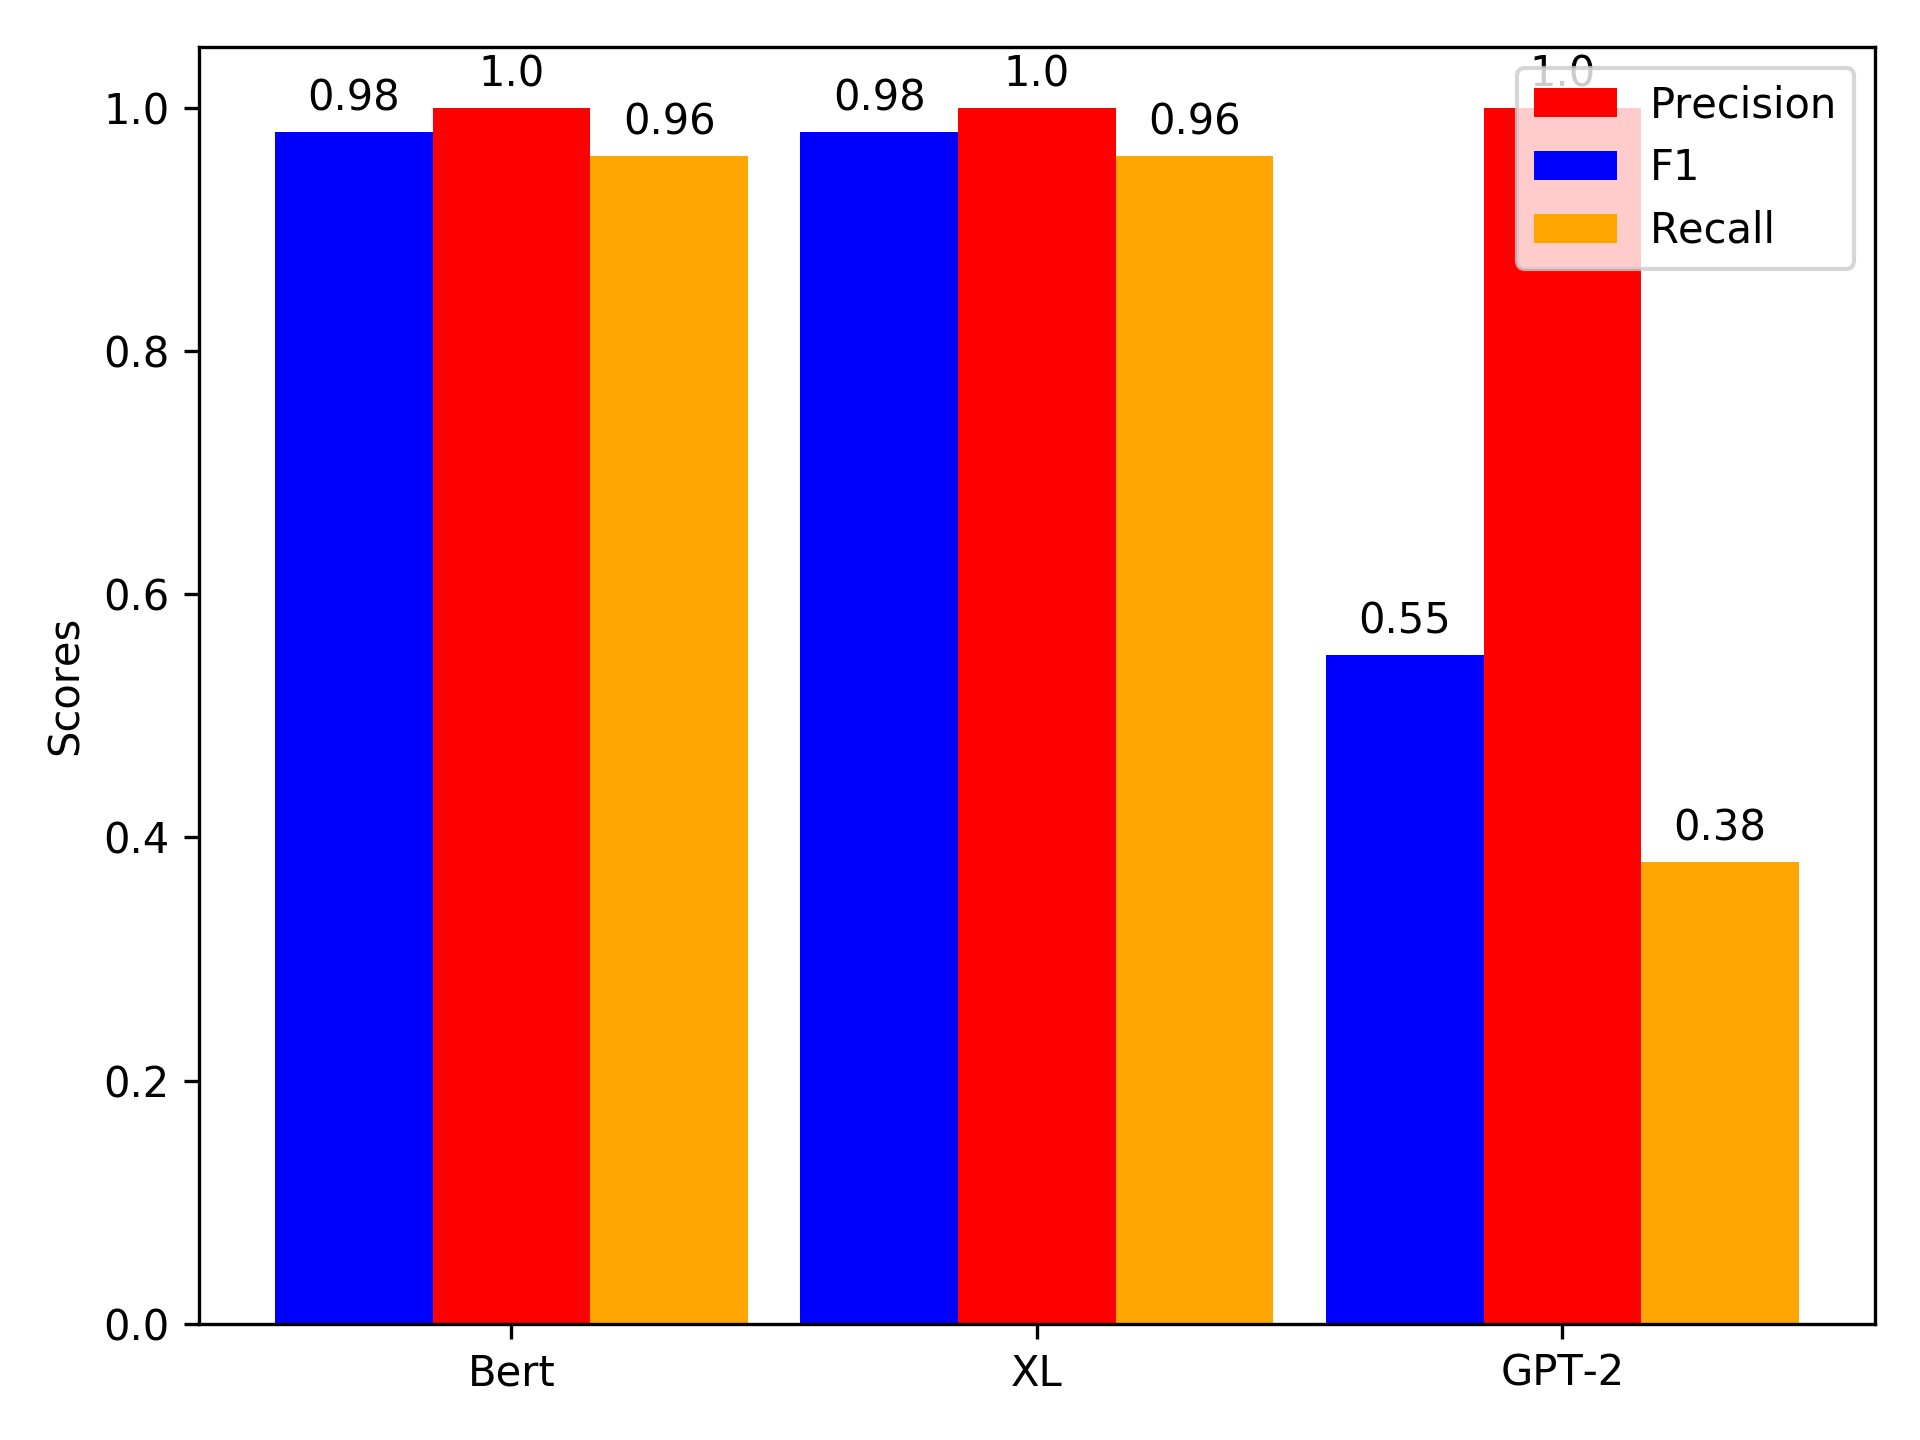
\includegraphics[width=6cm,height=4.5cm]{results/regression_sequence/regression_reverse.png}\\
  \caption{Scores for detecting reversed order of log events, using regression.}
  \label{fig:regression_reverse_order}
\end{figure}
\end{comment}

\begin{figure*}[ht!]
  \centering
  \captionsetup{justification=centering}
   \subfloat[5\% alteration\label{fig:results_regression_sequential_5}]{%
      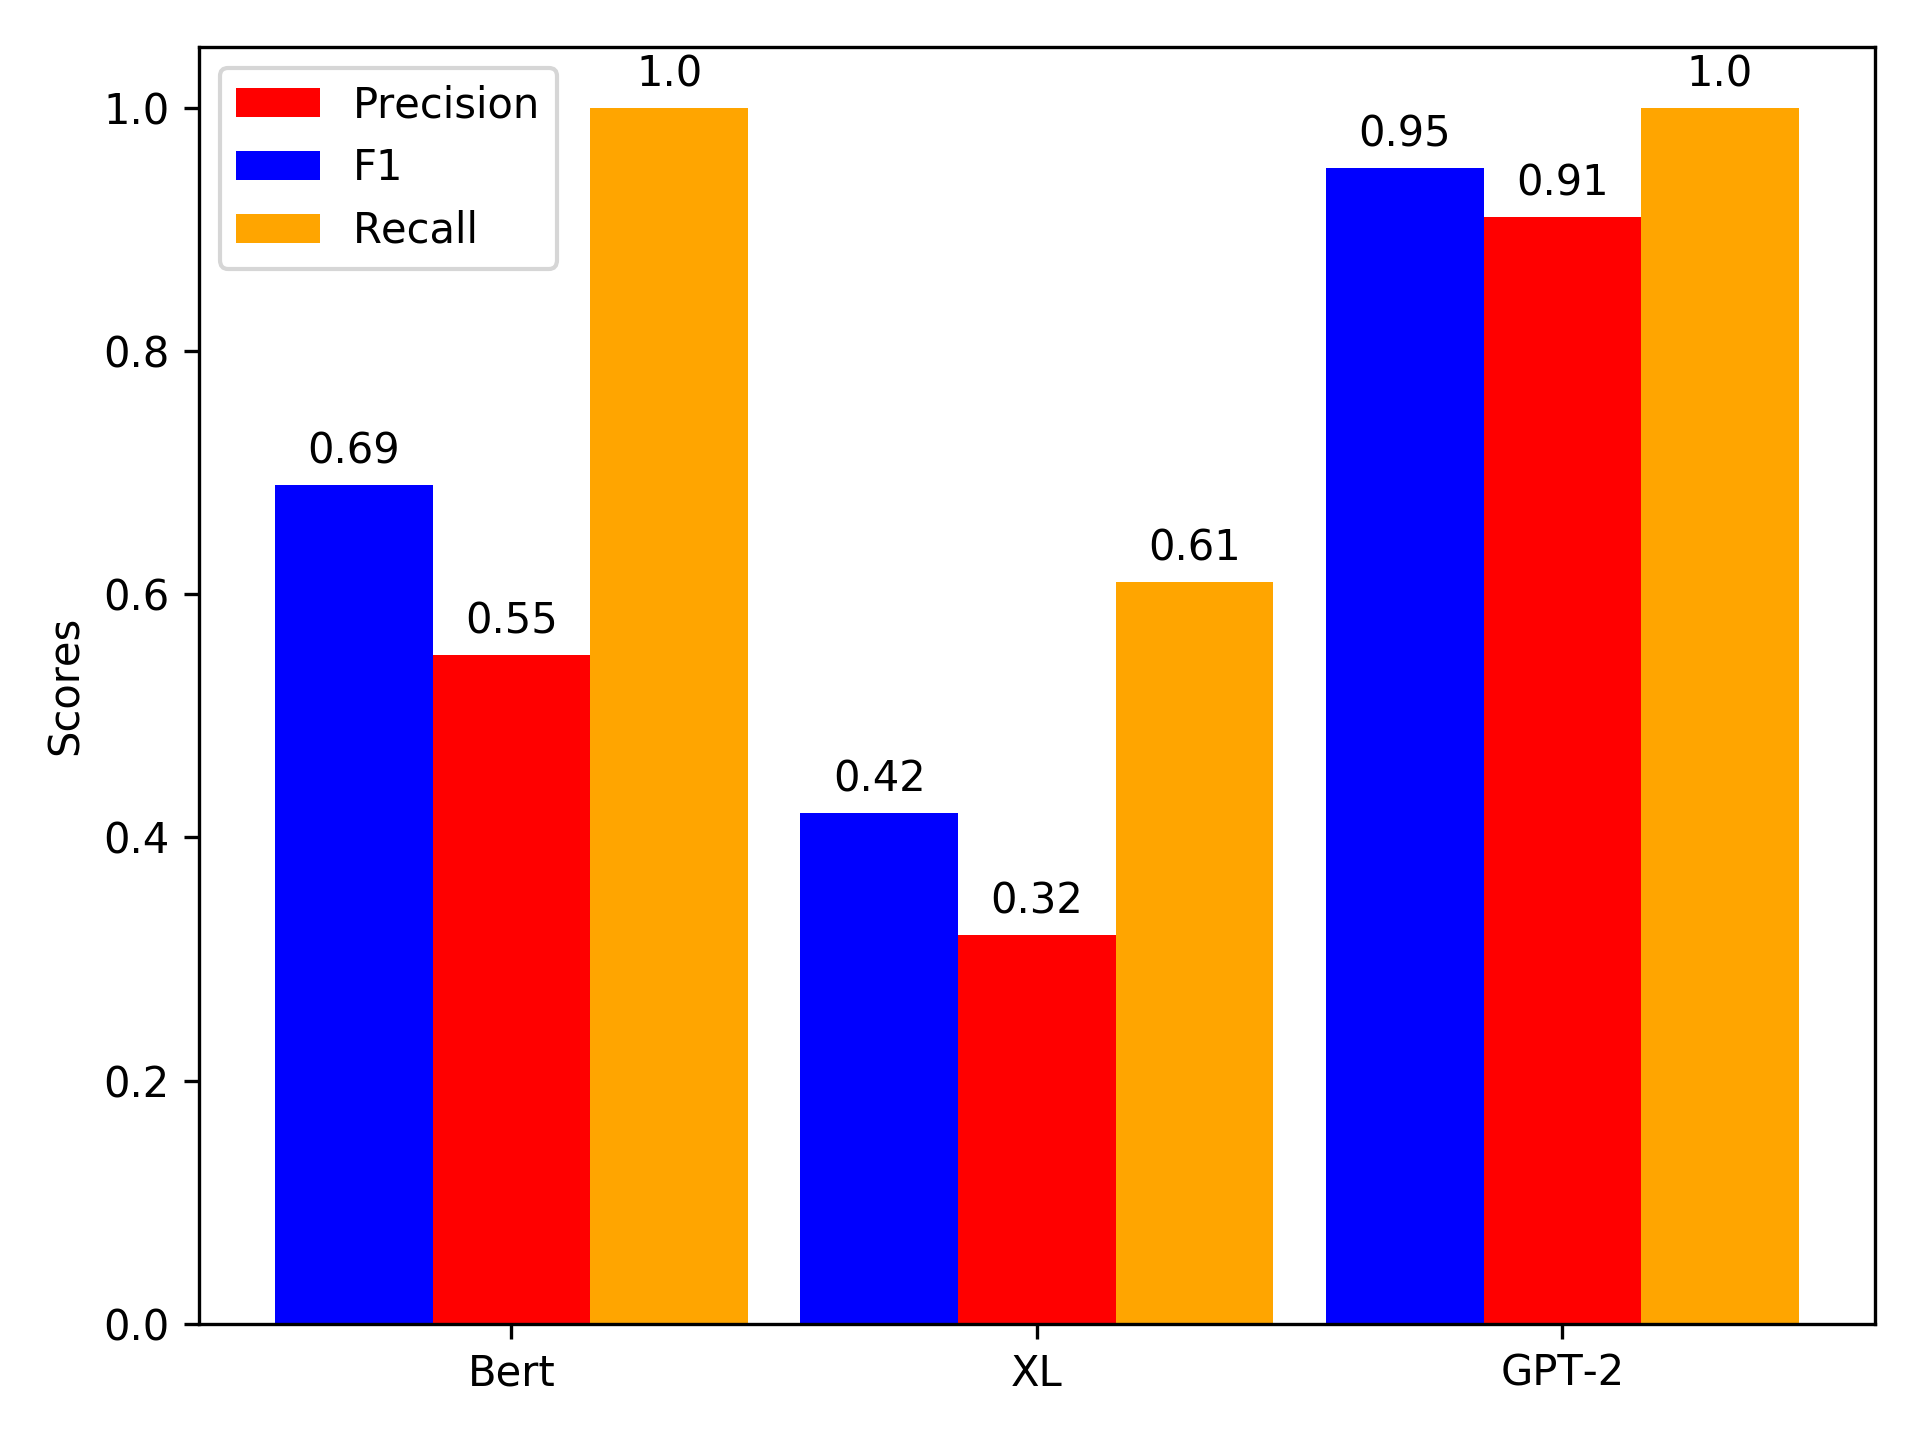
\includegraphics[trim={1cm 0.5cm 0cm 1cm}, width=0.322\textwidth]{results/average/regression_sequential_average_ratio_0.05.png}}
\hspace{\fill}
   \subfloat[10\% alteration\label{fig:results_regression_sequential_10} ]{%
      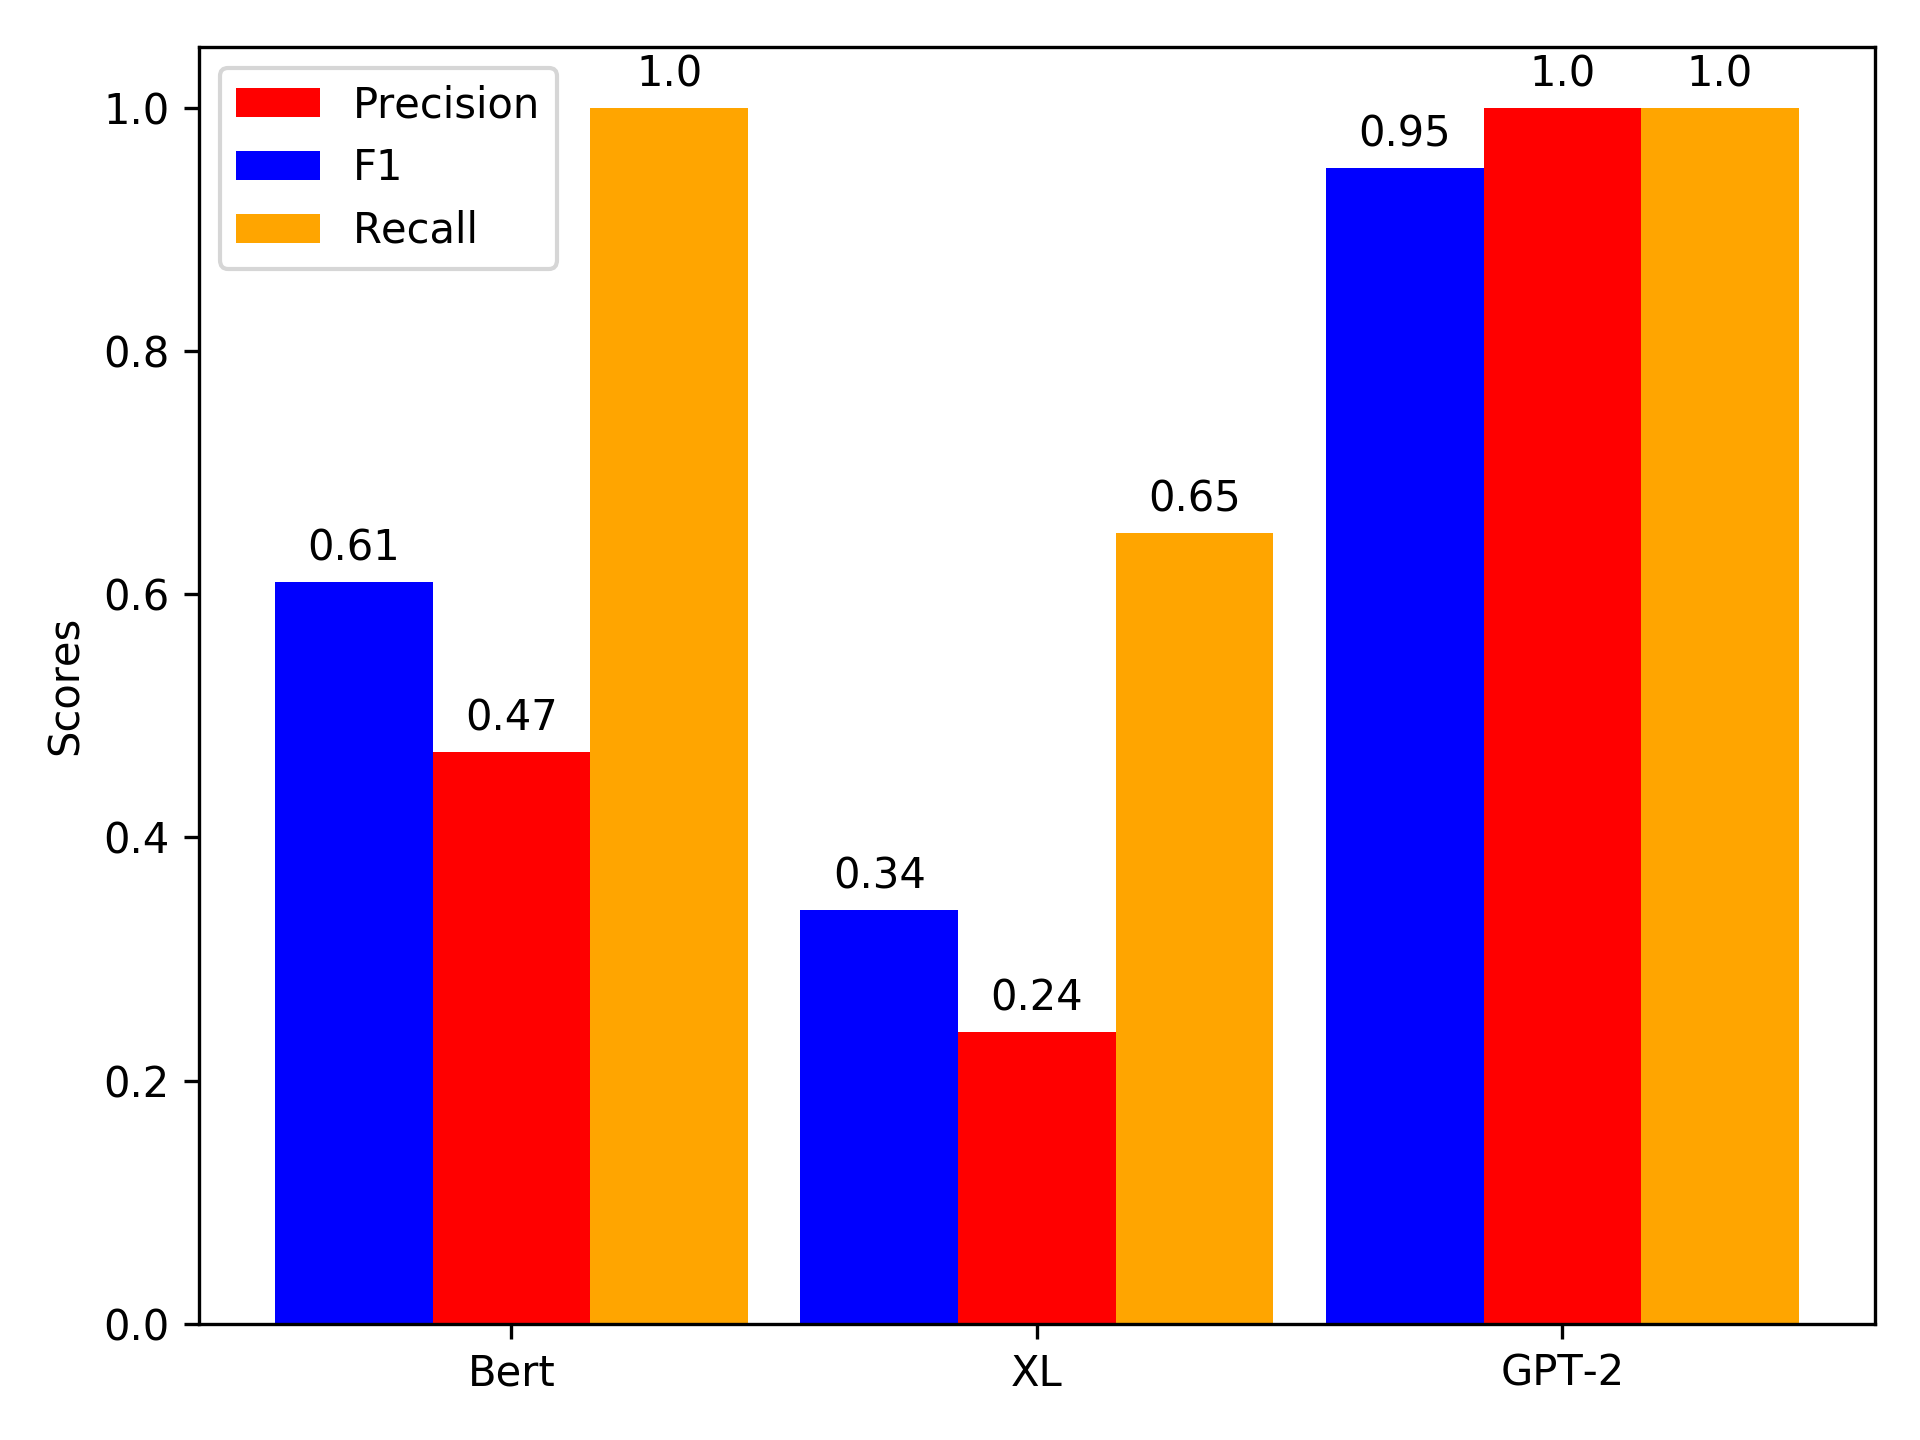
\includegraphics[trim={1cm 0.5cm 0cm 1cm}, width=0.322\textwidth]{results/average/regression_sequential_average_ratio_0.10.png}}
\hspace{\fill}
   \subfloat[15\% alteration\label{fig:results_regression_sequential_15}]{%
      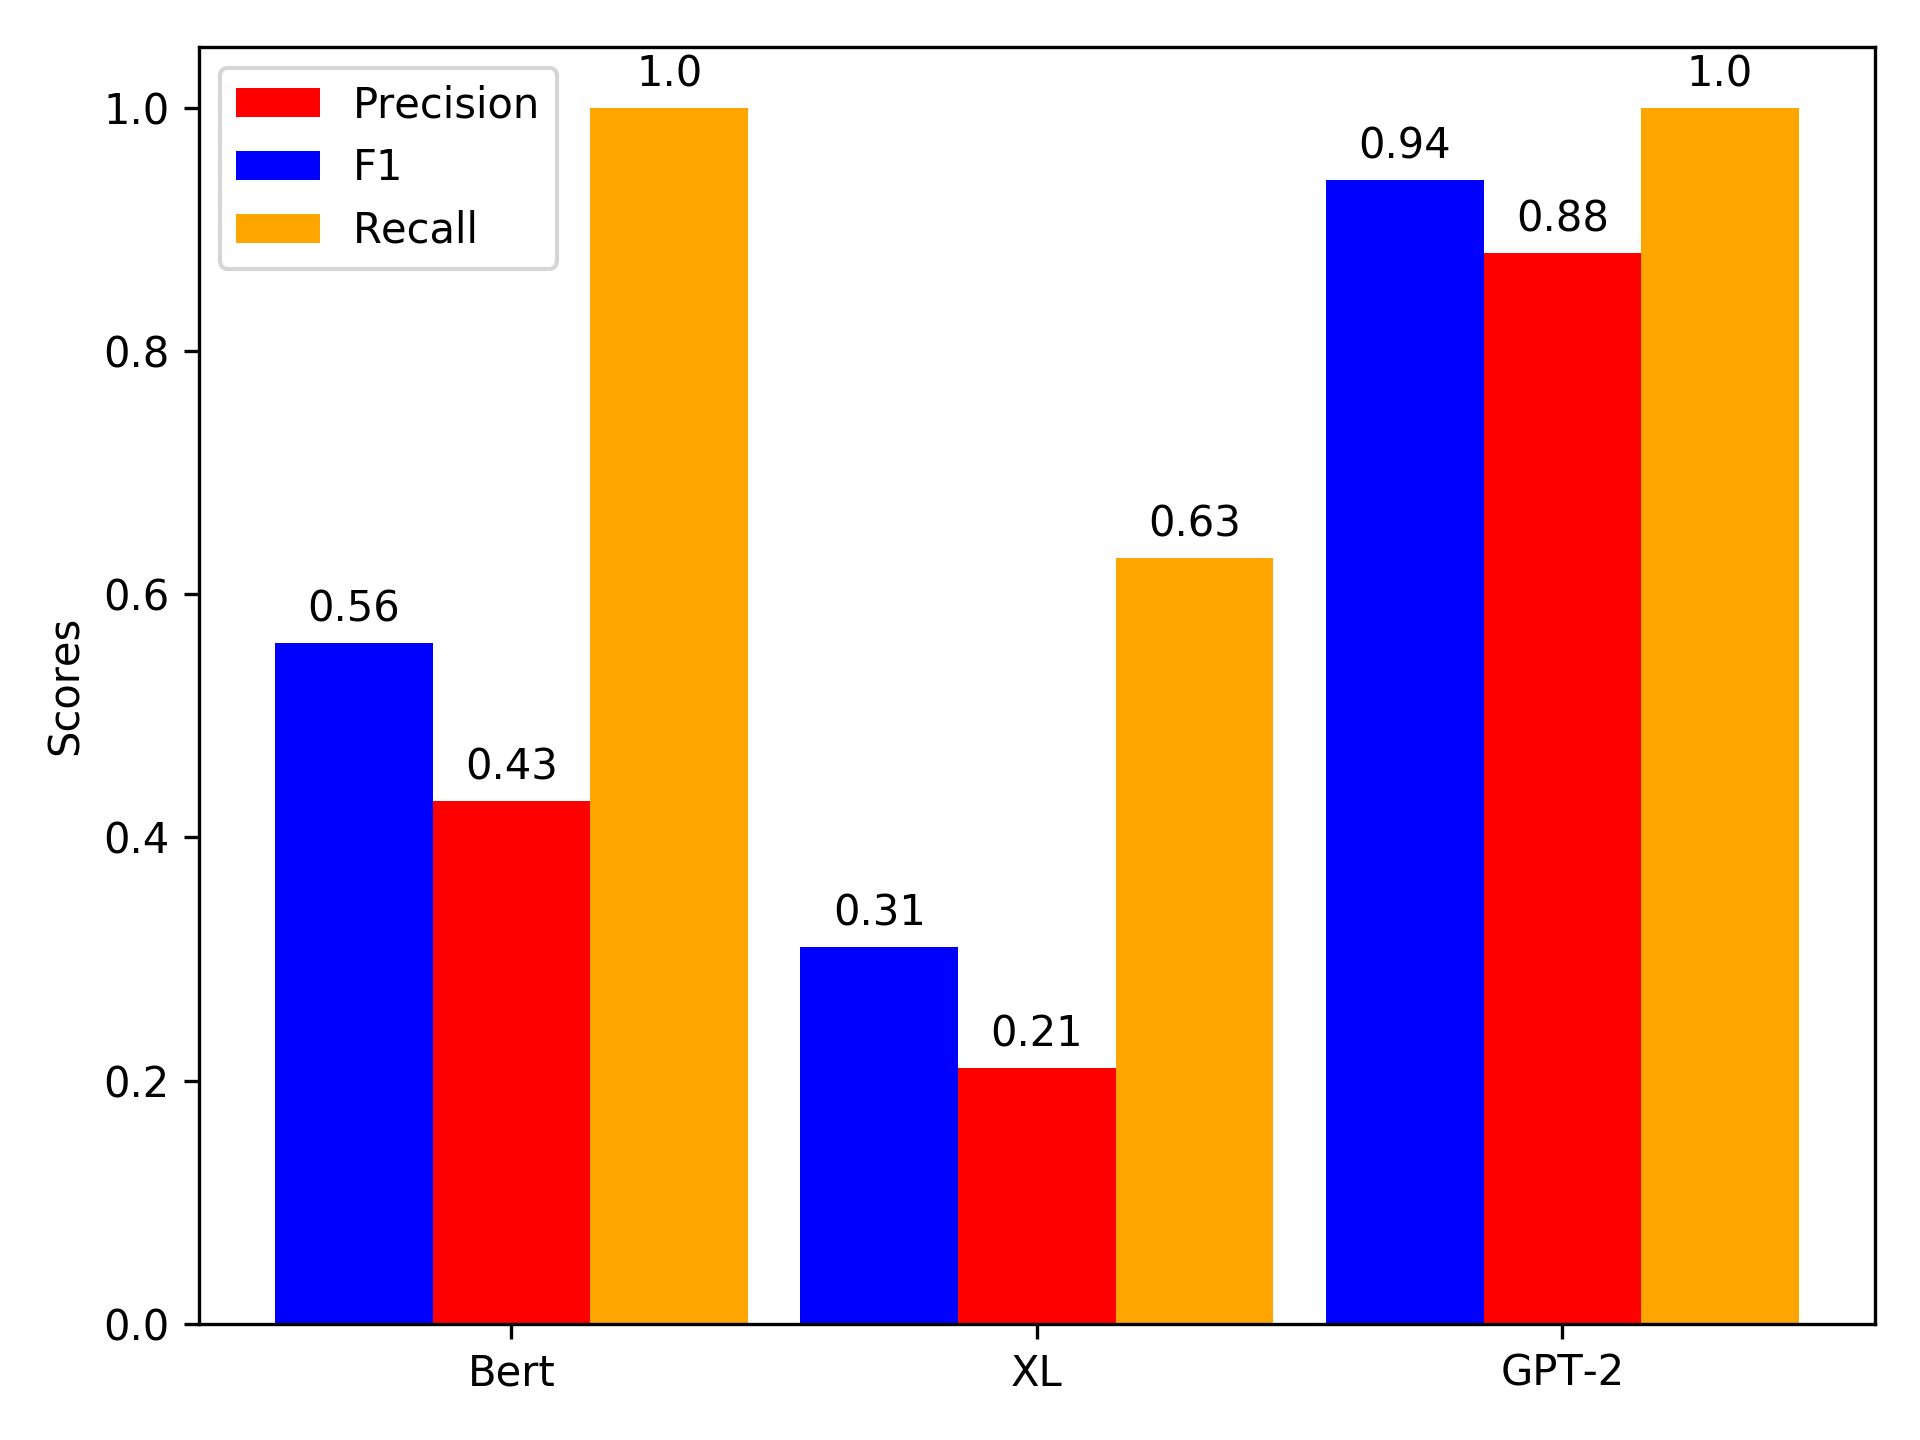
\includegraphics[trim={1cm 0.5cm 0cm 1cm}, width=0.322\textwidth]{results/average/regression_sequential_average_ratio_0.15.png}}\\
\caption{\label{fig:results_regression_sequential}Altering the sequences of logs at different ratios, inject semantically different anomalies, using regression.}
\end{figure*}


\begin{figure*}[ht!]
  \centering
  \captionsetup{justification=centering}
   \subfloat[5\% alteration\label{fig:results_regression_qualitative_5}]{%
      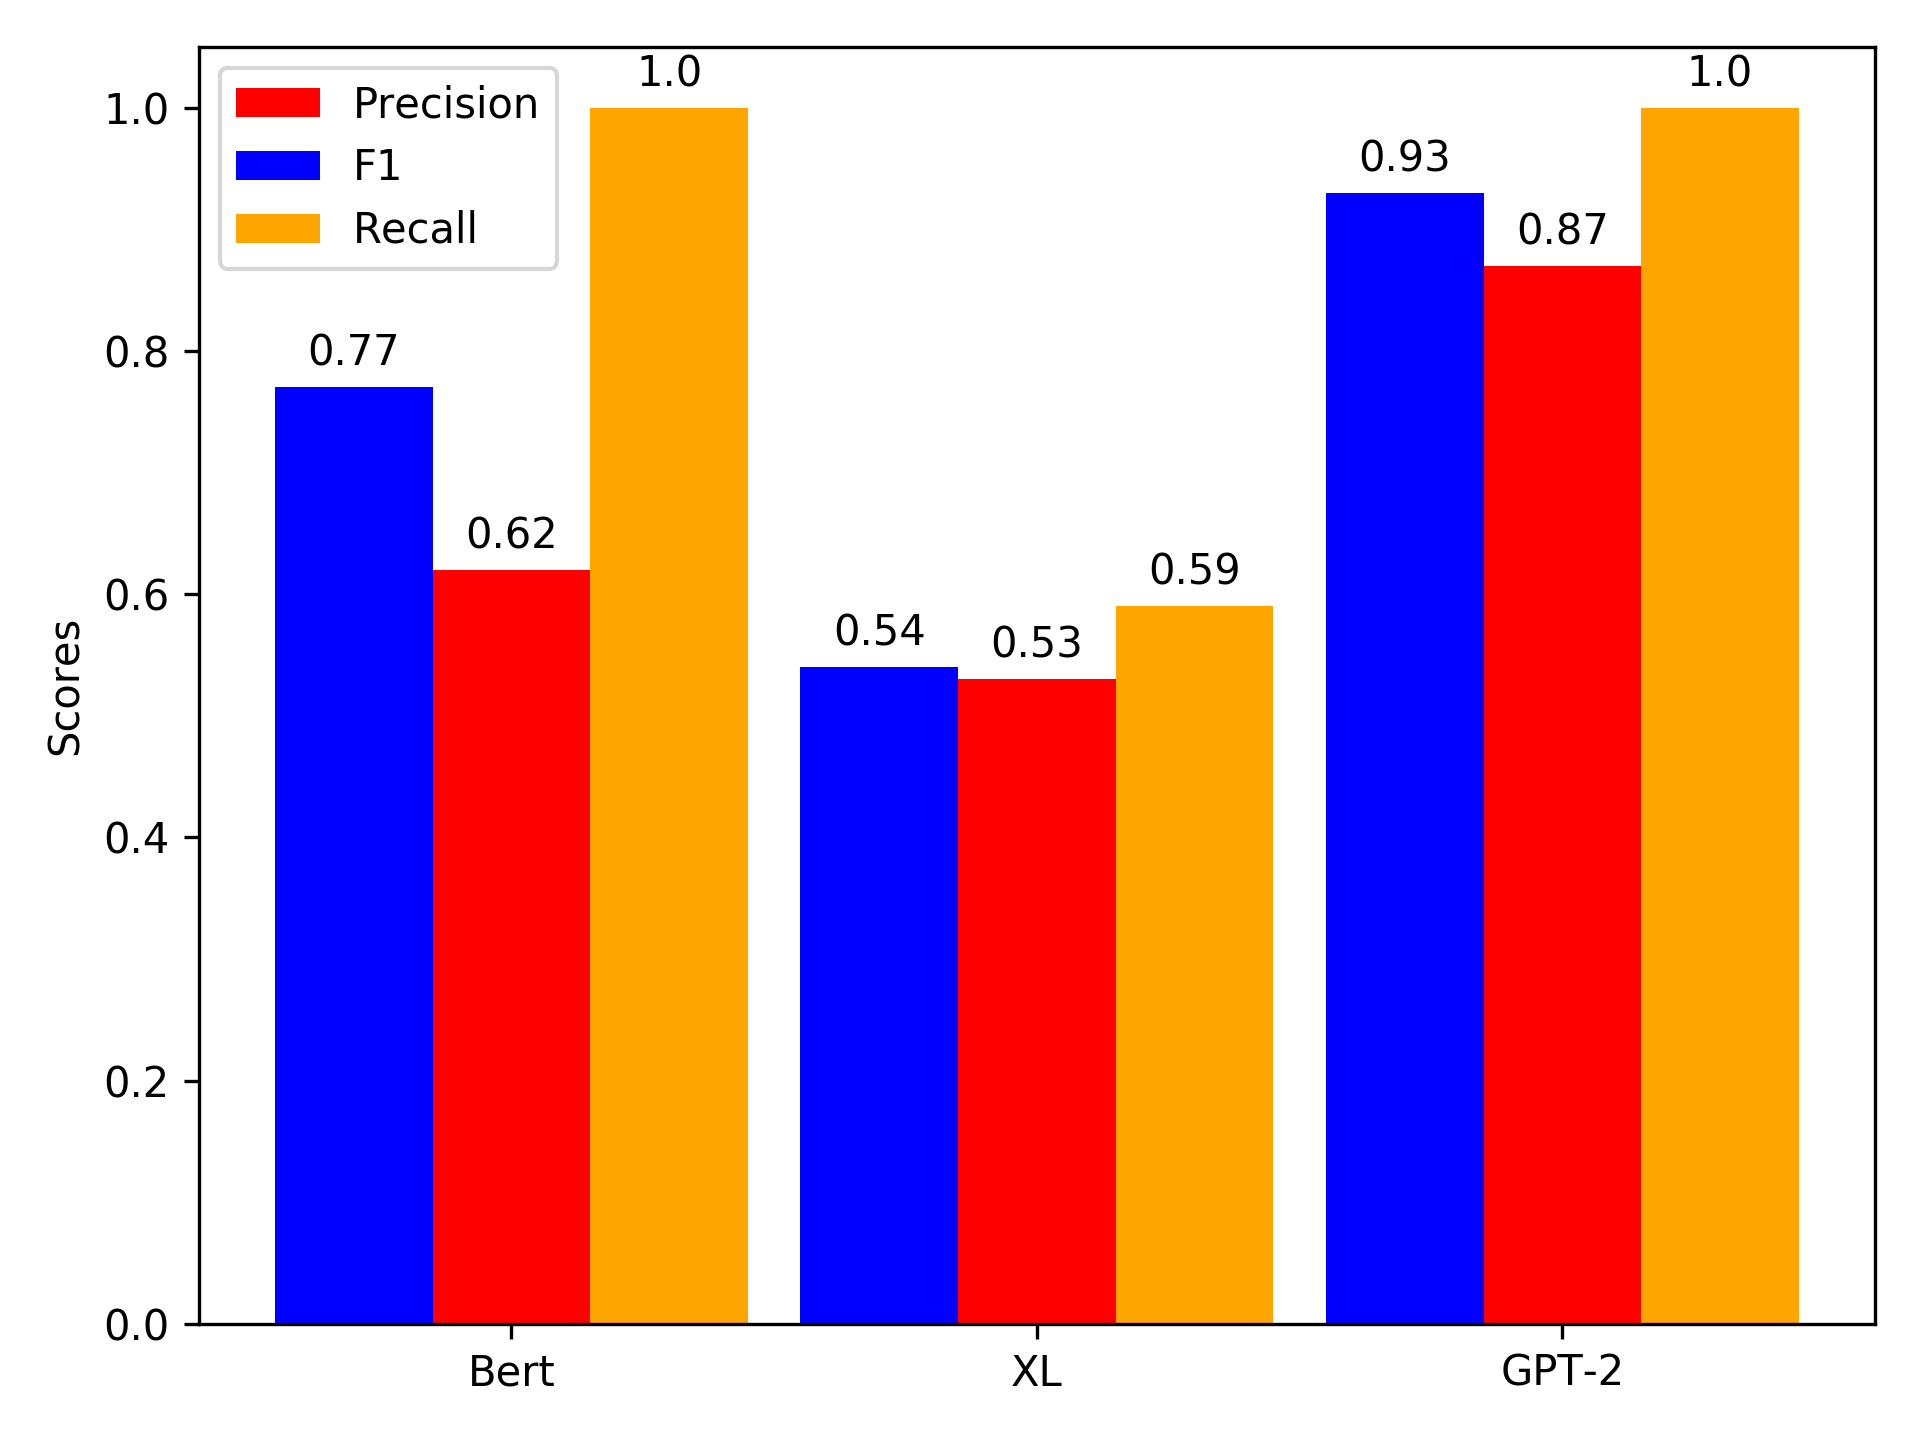
\includegraphics[trim={1cm 0.5cm 0cm 1cm}, width=0.322\textwidth]{results/average/regression_qualitative_average_ratio_0.05.png}}
\hspace{\fill}
   \subfloat[10\% alteration\label{fig:results_regression_qualitative_10} ]{%
      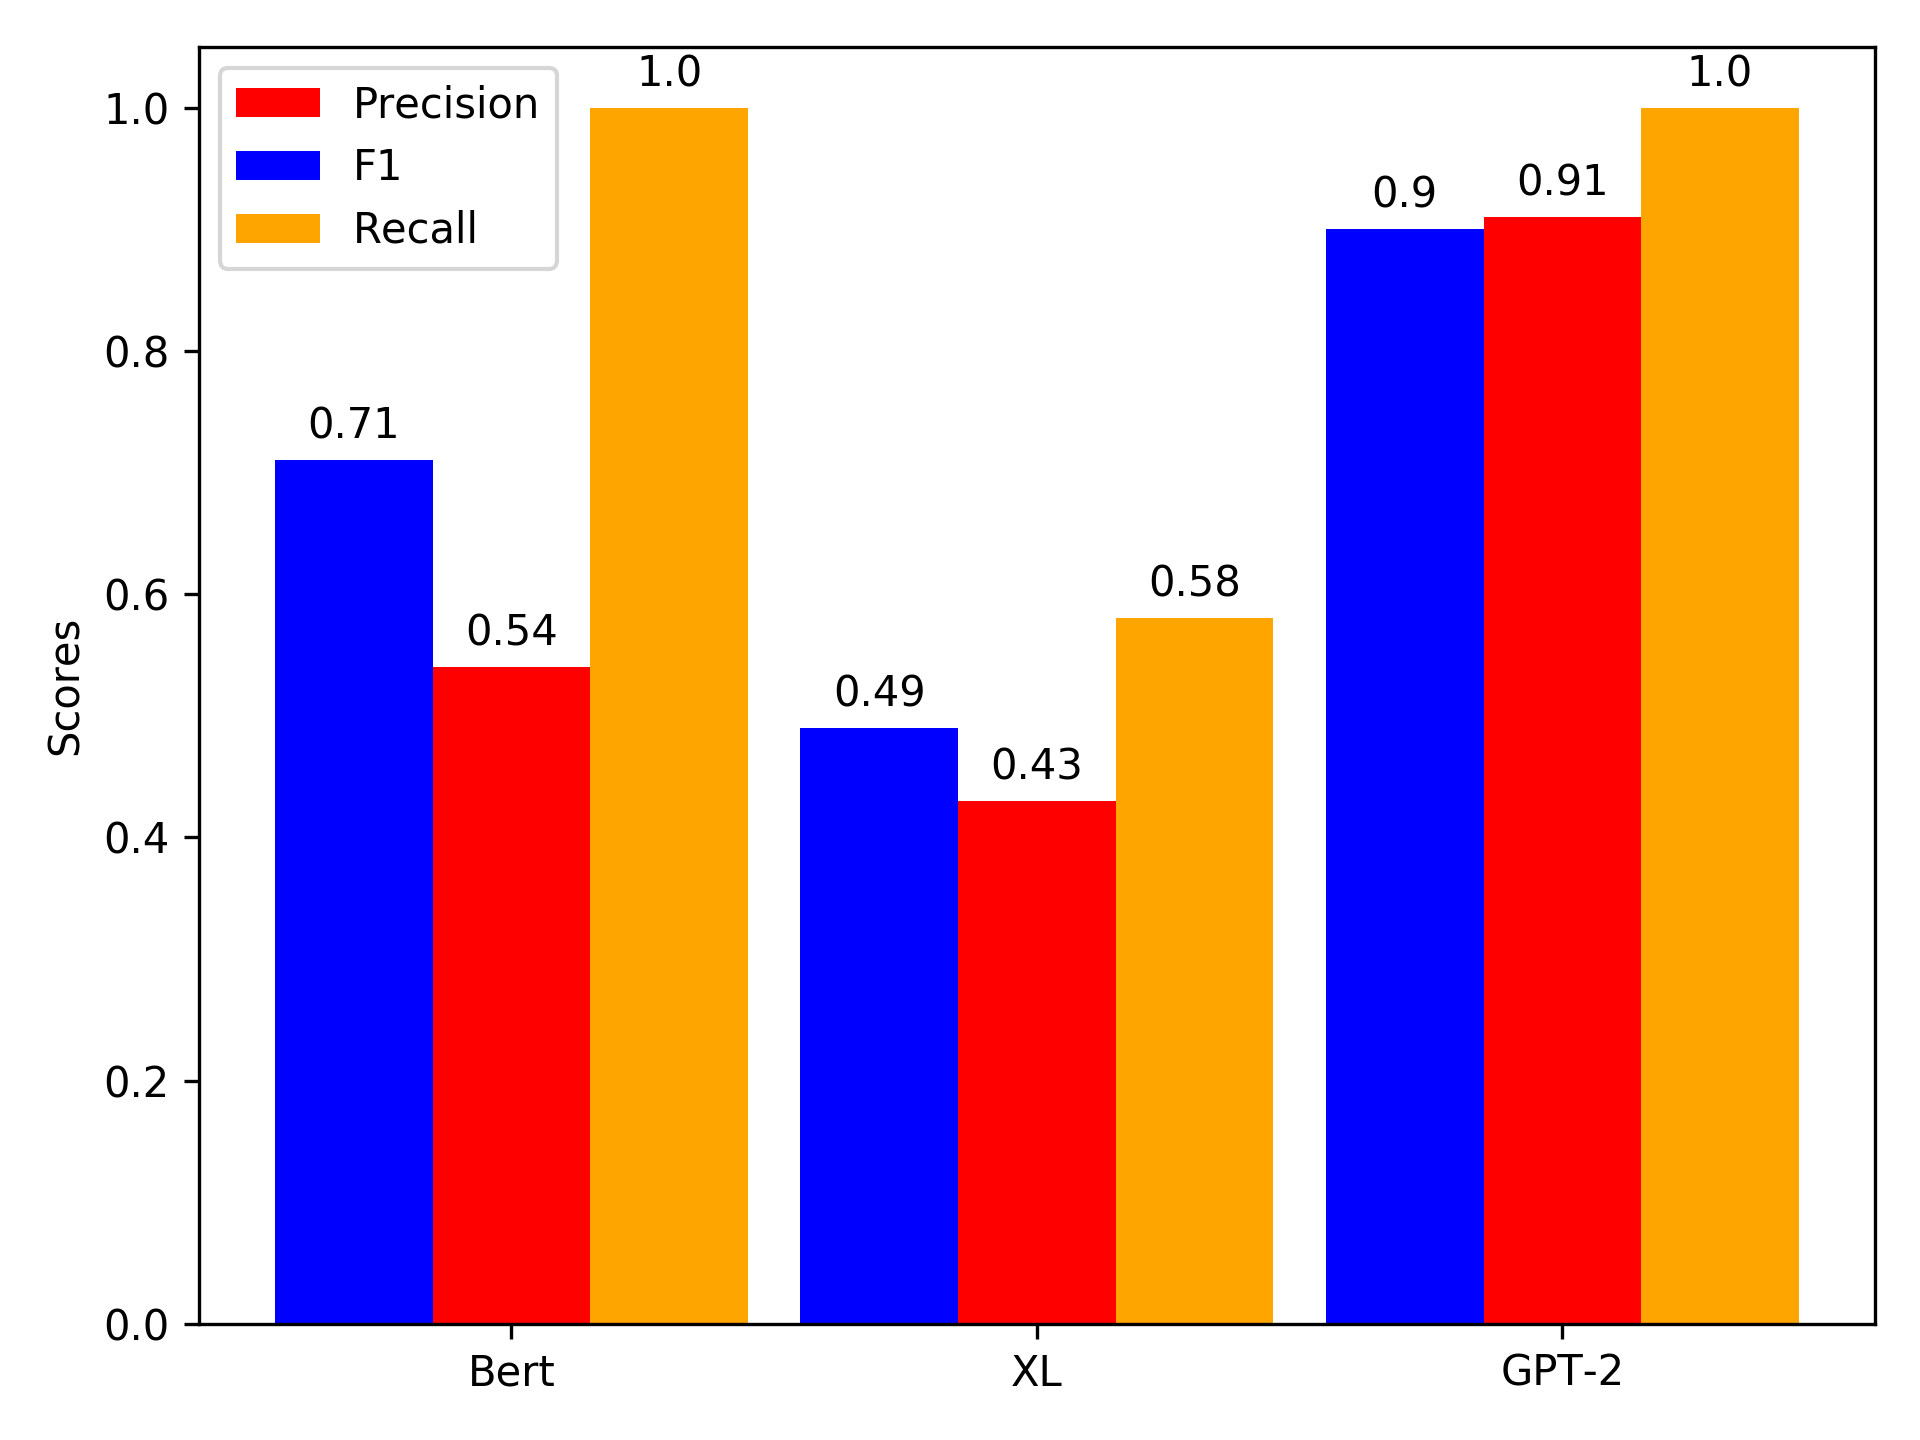
\includegraphics[trim={1cm 0.5cm 0cm 1cm}, width=0.322\textwidth]{results/average/regression_qualitative_average_ratio_0.10.png}}
\hspace{\fill}
   \subfloat[15\% alteration\label{fig:results_regression_qualitative_15}]{%
      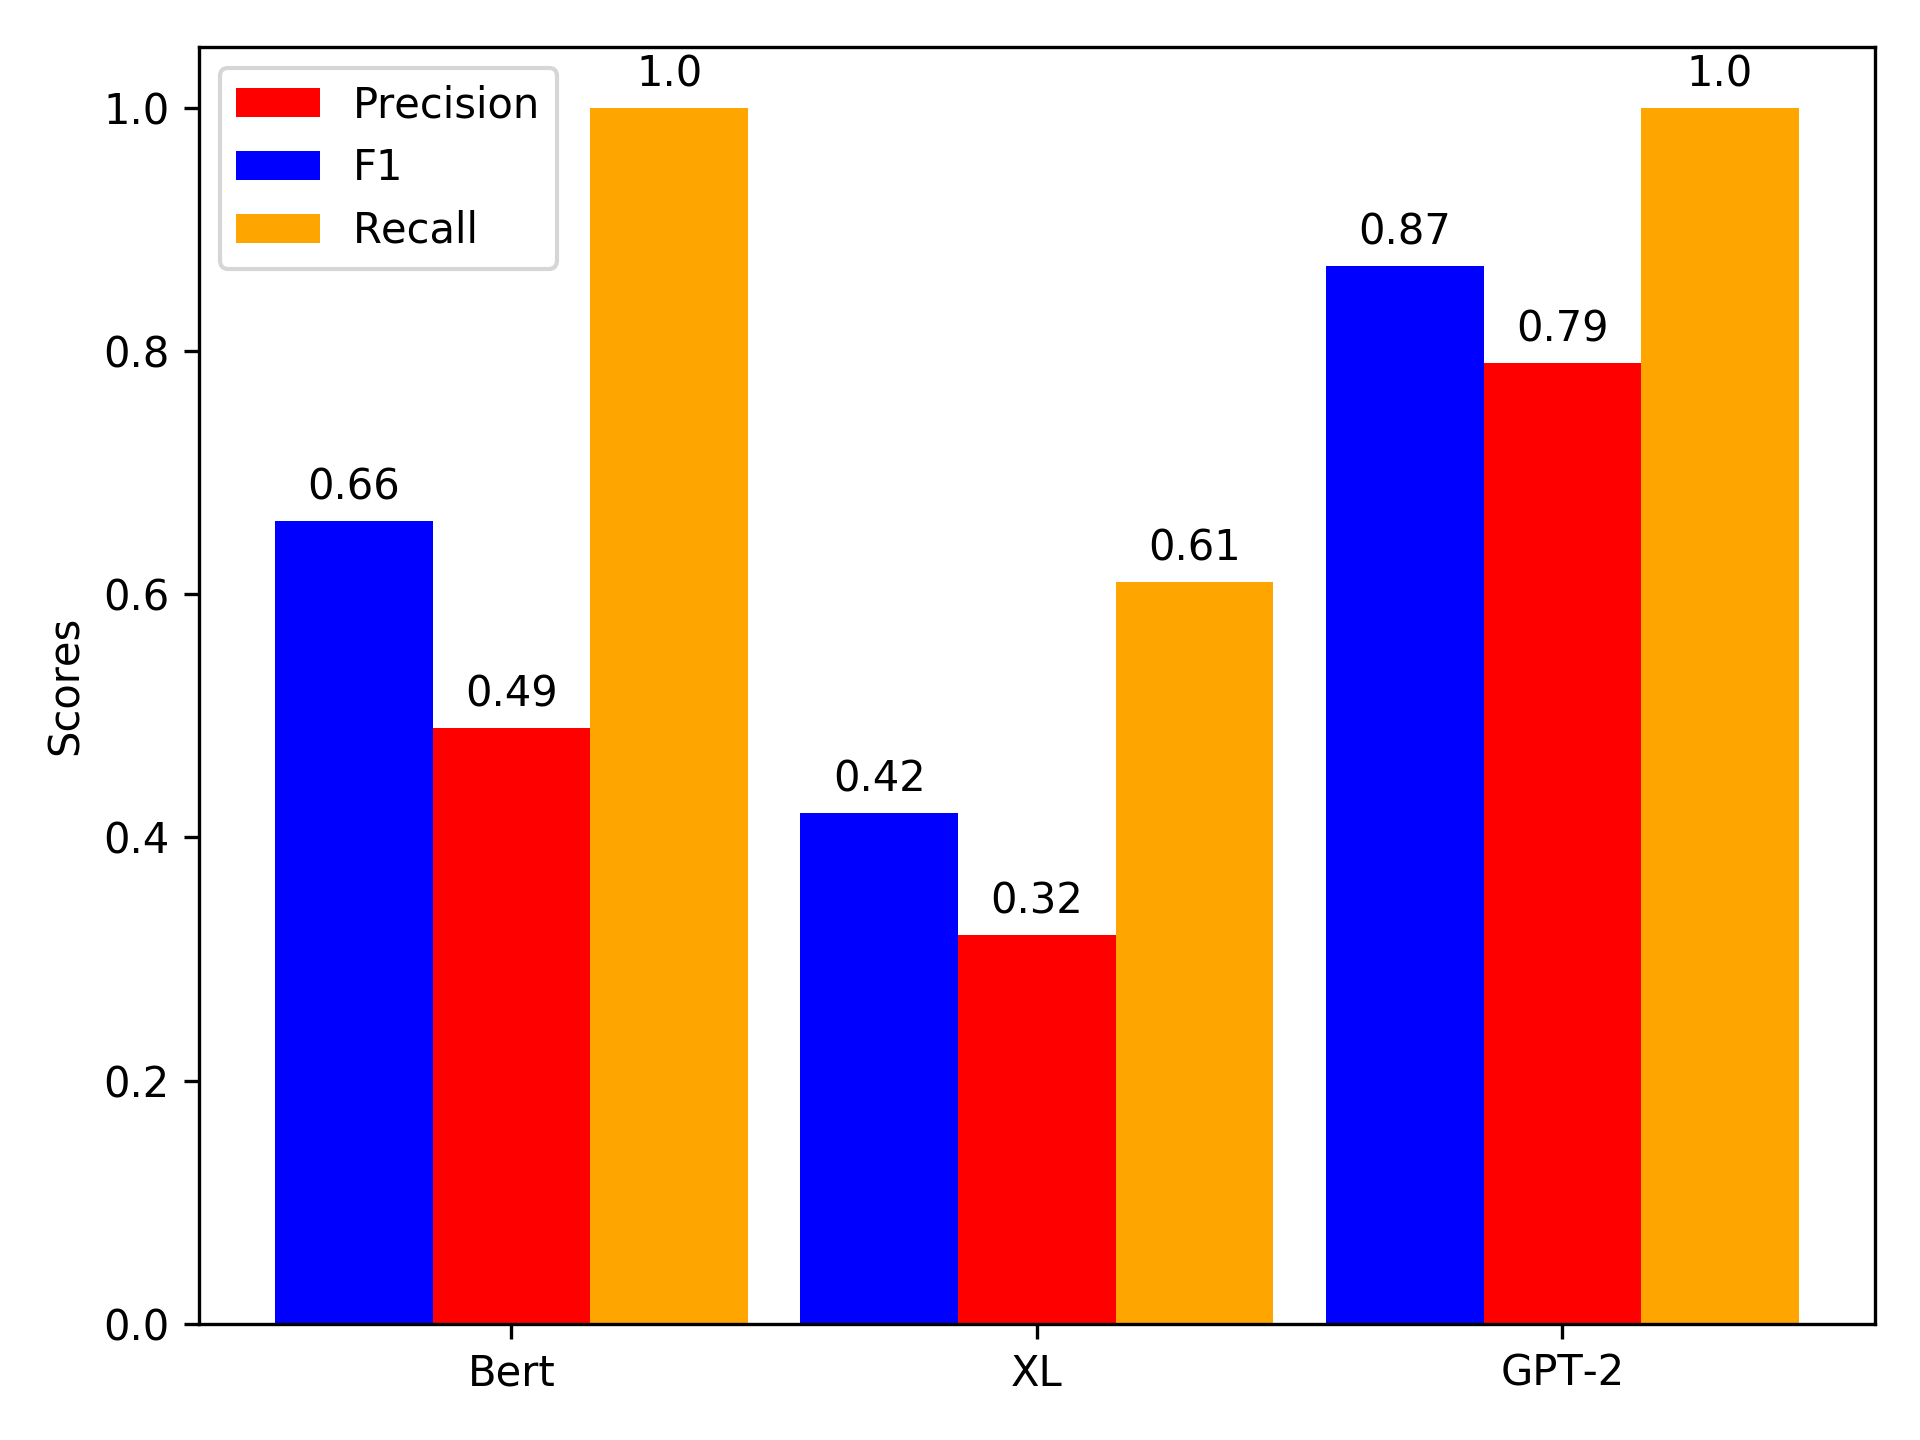
\includegraphics[trim={1cm 0.5cm 0cm 1cm}, width=0.322\textwidth]{results/average/regression_qualitative_average_ratio_0.15.png}}\\
\caption{\label{fig:results_regression_words}Altering log lines at different ratios, inject semantically different anomalies, using regression.}
\end{figure*}	

%%%%%

\begin{figure}[H]
  \centering
  \captionsetup{justification=centering}
  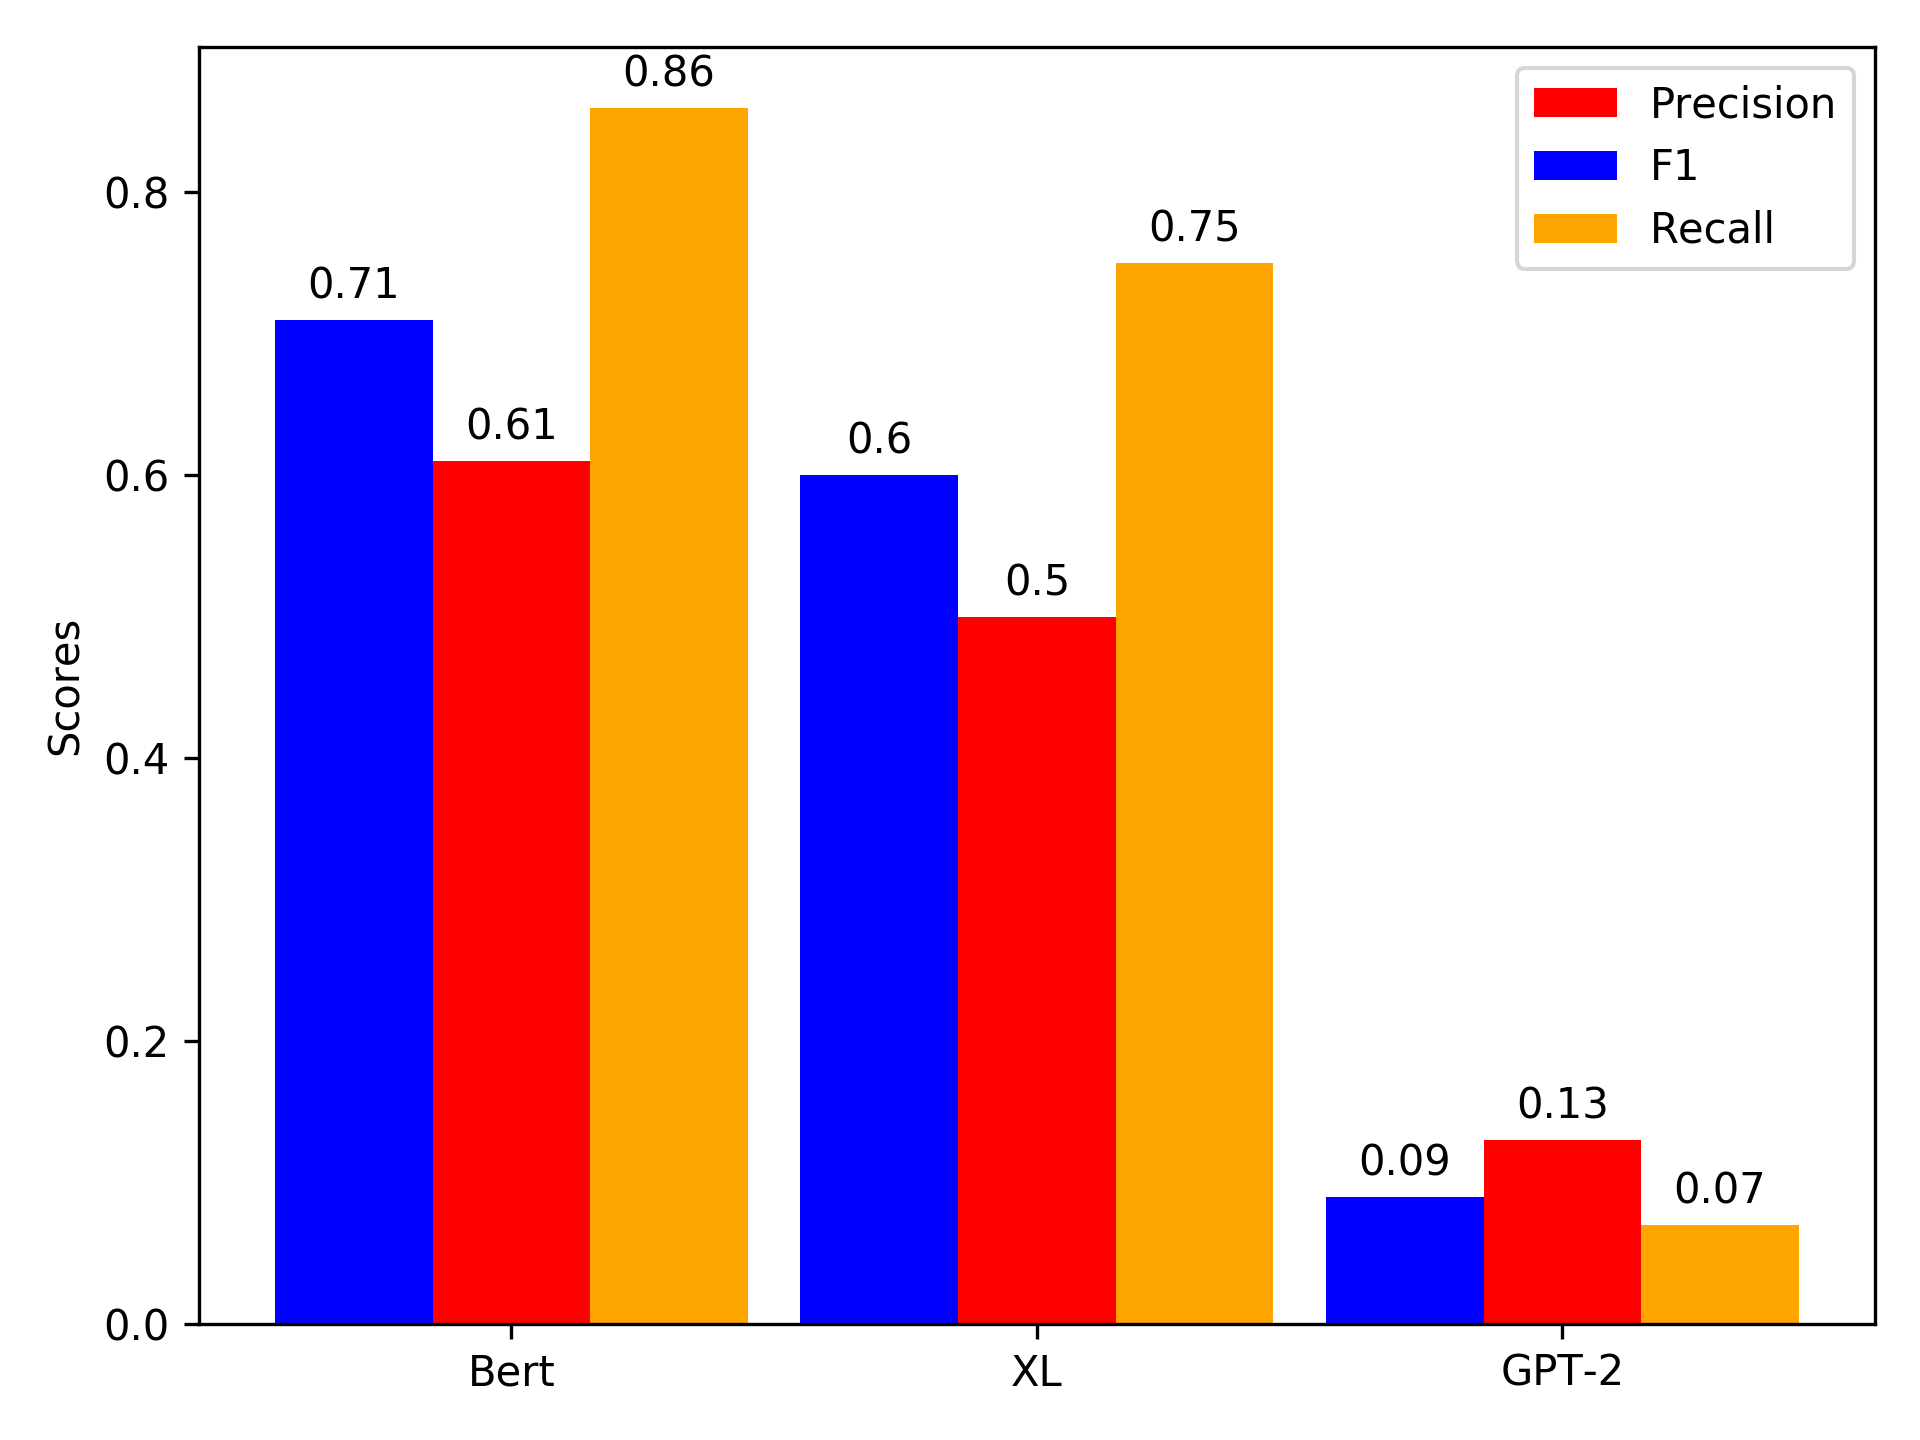
\includegraphics[width=8cm]{results/regression_replace_half.png}\\
  \caption{Inject semantically similar anomalies, using regression.}
  \label{fig:replace_words_regression}
\end{figure}

\begin{figure}[H]
  \centering
  \captionsetup{justification=centering}
  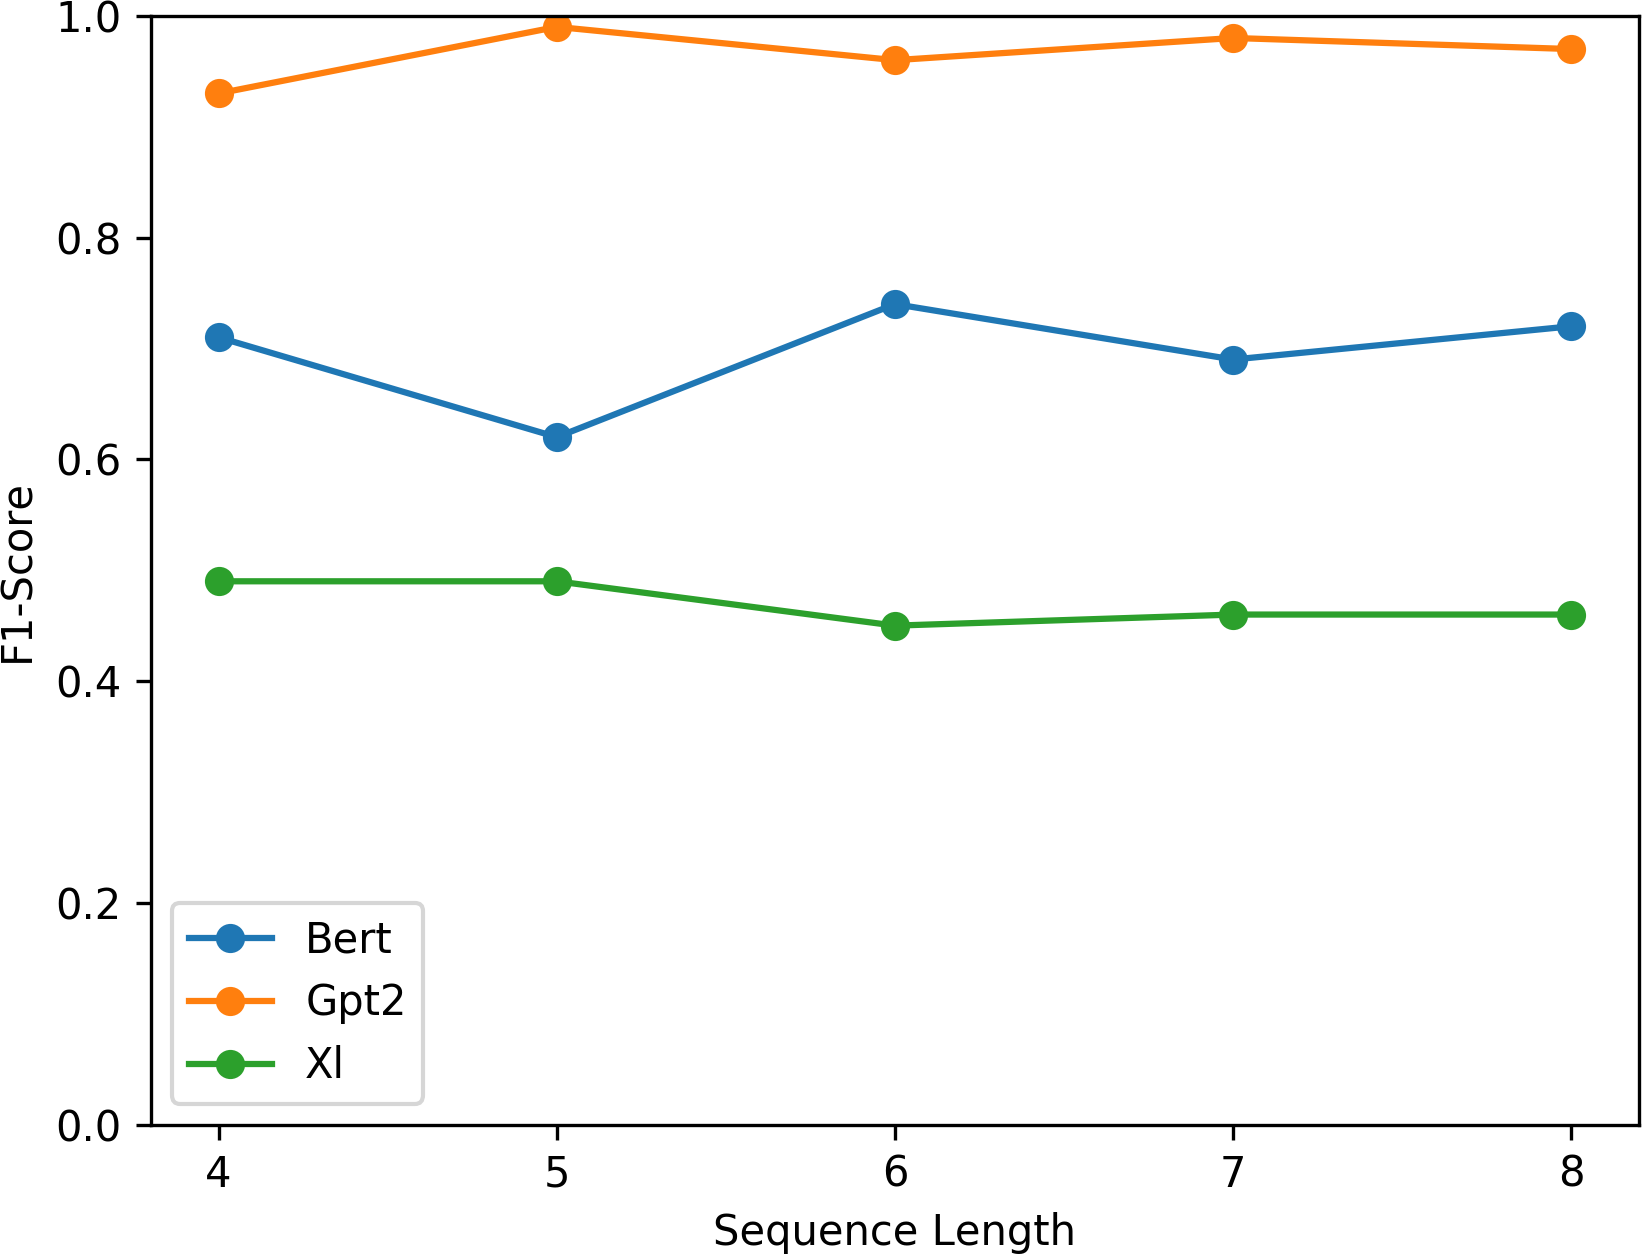
\includegraphics[width=7.7cm]{results/seq_len/sequence_len_regression.png}\\
  \caption{F1-Score for varying input sequence lengths, for 15\% of the log lines insert one word as alteration, inject semantically different anomalies, using regression.}
  \label{fig:seq_len_regression}
\end{figure}




\newpage
%%%%%%%%%%%%%%%%
% CLASSIFICATION 
%%%%%%%%%%%%%%%%
\subsection{Classification\label{sec:results-classification}}
In this subsection, the results of the classification-based approach are presented, under the exact same conditions as in \ref{sec:results-regression}. 
The ability of the system to detect semantically different anomalies, despite alterations on the sequences of logs, i.e. deleting, shuffling and duplicating events, can be seen in \ref{fig:results_multiclass_sequential}. For the classification-based approach a different picture becomes apparent than for the regression-based approach, where GPT-2 showed better results for the injection of semantically different anomalies. For classification though, Bert and XL-Transformers show recall values of 1.0 throughout, where GPT-2 only reaches recall values of around 0.7. Bert achieves a F1-scores of 0.67 for 5\% alterations, 0.59 for 10\% alterations and 0.54 for 15\% alterations, while XL-Transformers achieves 0.51 for 5\%, 0.45 for 10\% and 0.41 for 15\% alterations, and GPT-2 achieves 0.44 for 5\% alterations, 0.39 for 10\% alterations, and 0.36 for 15\% alterations. For precision, Bert achieves 0.37 for 15\% alterations, XL-Transformers 0.25 and GPT-2 0.24.
Bert shows the best F1-score and precision throughout, followed by XL-Transformers and GPT-2.

The impacts of alterations on the logs themselves, i.e. inserting, removing and replacing words are summarised in figure \ref{fig:results_multiclass_qualitative}, where semantically different anomalies are injected. As mentioned above, only averaged results on the individual injections are presented. Results broken down by each alteration can be found in the appendix \ref{appendix:classification}.
Here it becomes evident again, similarly to the results for the regression-based approach, that both Bert and XL-Transformers perform better for the detection of semantically different anomalies with alterations on the logs themselves than alterations on the sequences of logs, while GPT-2 performs slightly worse when these two categories are compared. Once again, as for the alterations on the log sequences, Bert and XL-Transformers both achieve a recall value of 1.0, while GPT-2 achieves a recall value of around 0.7 for all alteration ratios. Bert achieves a F1-score of 0.77 for 5\% alterations, 0.7 for 10\% alterations and 0.67 for 15 \% alterations. XL-Transformers achieves a F1-score of 0.58 for 5\% alterations, 0.55 for 10\% alterations and 0.53 for 15\% alterations. GPT-2 achieves F1-scores of 0.53 for 5\% alterations, 0.46 for 10\% alterations, and 0.43 for 15\% alterations. For precision, Bert achieves a value of 0.63 for 5\% alterations, 0.53 for 10\% alterations and 0.5 for 15\% alterations. XL-Transformers achieves a precision of 0.41 for 5\% alterations, 0.38 for 10\% alterations and 0.36 for 15\% alterations. GPT-2 achieves 0.43 for 5\% alterations, 0.34 for 10\% alterations and 0.31 for 15\% alterations.

Overall, it can be stated that Bert performs best for detecting semantically different results using the classification approach, followed by XL-Transformers and GPT-2.

The impact of the input sequence length on the F1-scores can be seen in \ref{fig:seq_len_classification}, where for 15\% of the log lines one word is inserted to simulate unstable logs, and 5\% semantically different anomalies are injected. Bert again seems to profit slightly from sequence lengths longer than 6, whereas the quality of results for XL-Transformers and GPT-2 seem to have a tendency to degrade in prediction quality for longer input sequence lengths. 

The results for injecting semantically similar anomalies can be seen in figure \ref{fig:replace_words_classification}. In comparison to the previous results, better F1-scores and precision are achieved by Bert, XL-Transformers and GPT-2. The results for recall stay essentially the same. While Bert is able to achieve a F1-score of 0.94, with 0.9 precision and recall of 1.0, XL-Transformers achieves a F1-score of 0.81, with 0.68 precision and recall of 1.0 and GPT-2 returns a F1-score of 0.71, precision of 0.73 and recall of 0.68, showing that Bert is able to detect semantically similar anomalies best, when using the classification approach.

Similarly to the results using regression, the classification approach for detecting semantically similar anomalies seems most fit for Bert and the least for GPT-2, yet GPT-2 is able to achieve much more useful results using the classification approach when detecting semantically similar anomalies, than using the regression approach, where it is the strongest detecting semantically different anomalies.



%\begin{figure}[h]
%  \centering
%  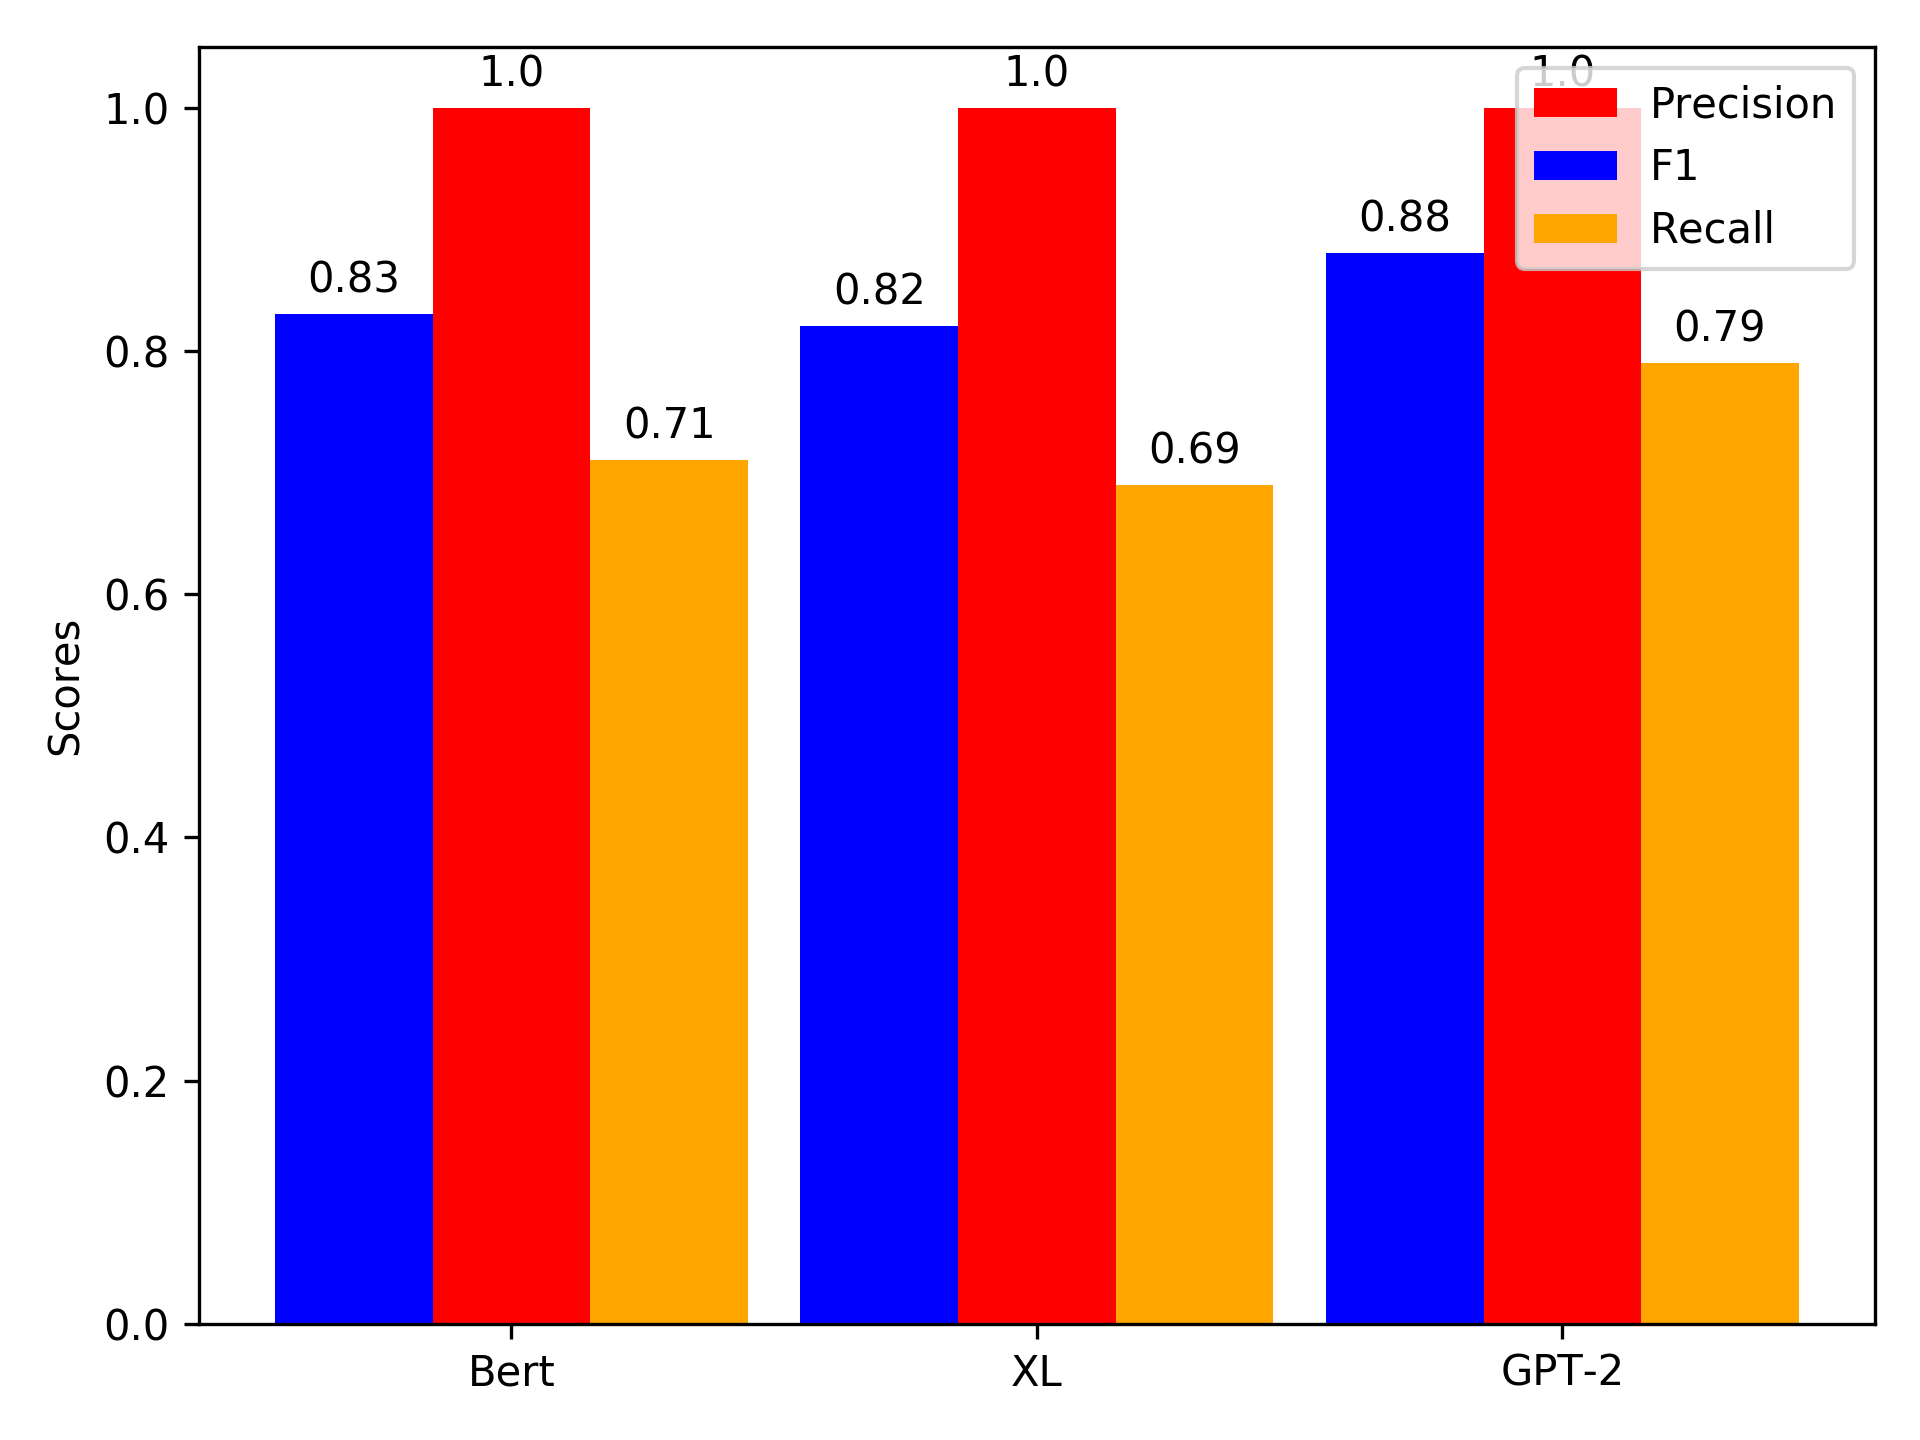
\includegraphics[width=6cm,height=4.5cm]{results/classification_sequence/multiclass_reverse.png}\\
%  \caption{Scores for detecting reversed order of log events, using classification.}
%  \label{fig:multiclass_reverse_order}
%\end{figure}
% multiclass sequential
\begin{figure*}[ht!]
  \centering
  \captionsetup{justification=centering}
   \subfloat[5\% alteration\label{fig:results_multiclass_sequential_5}]{%
      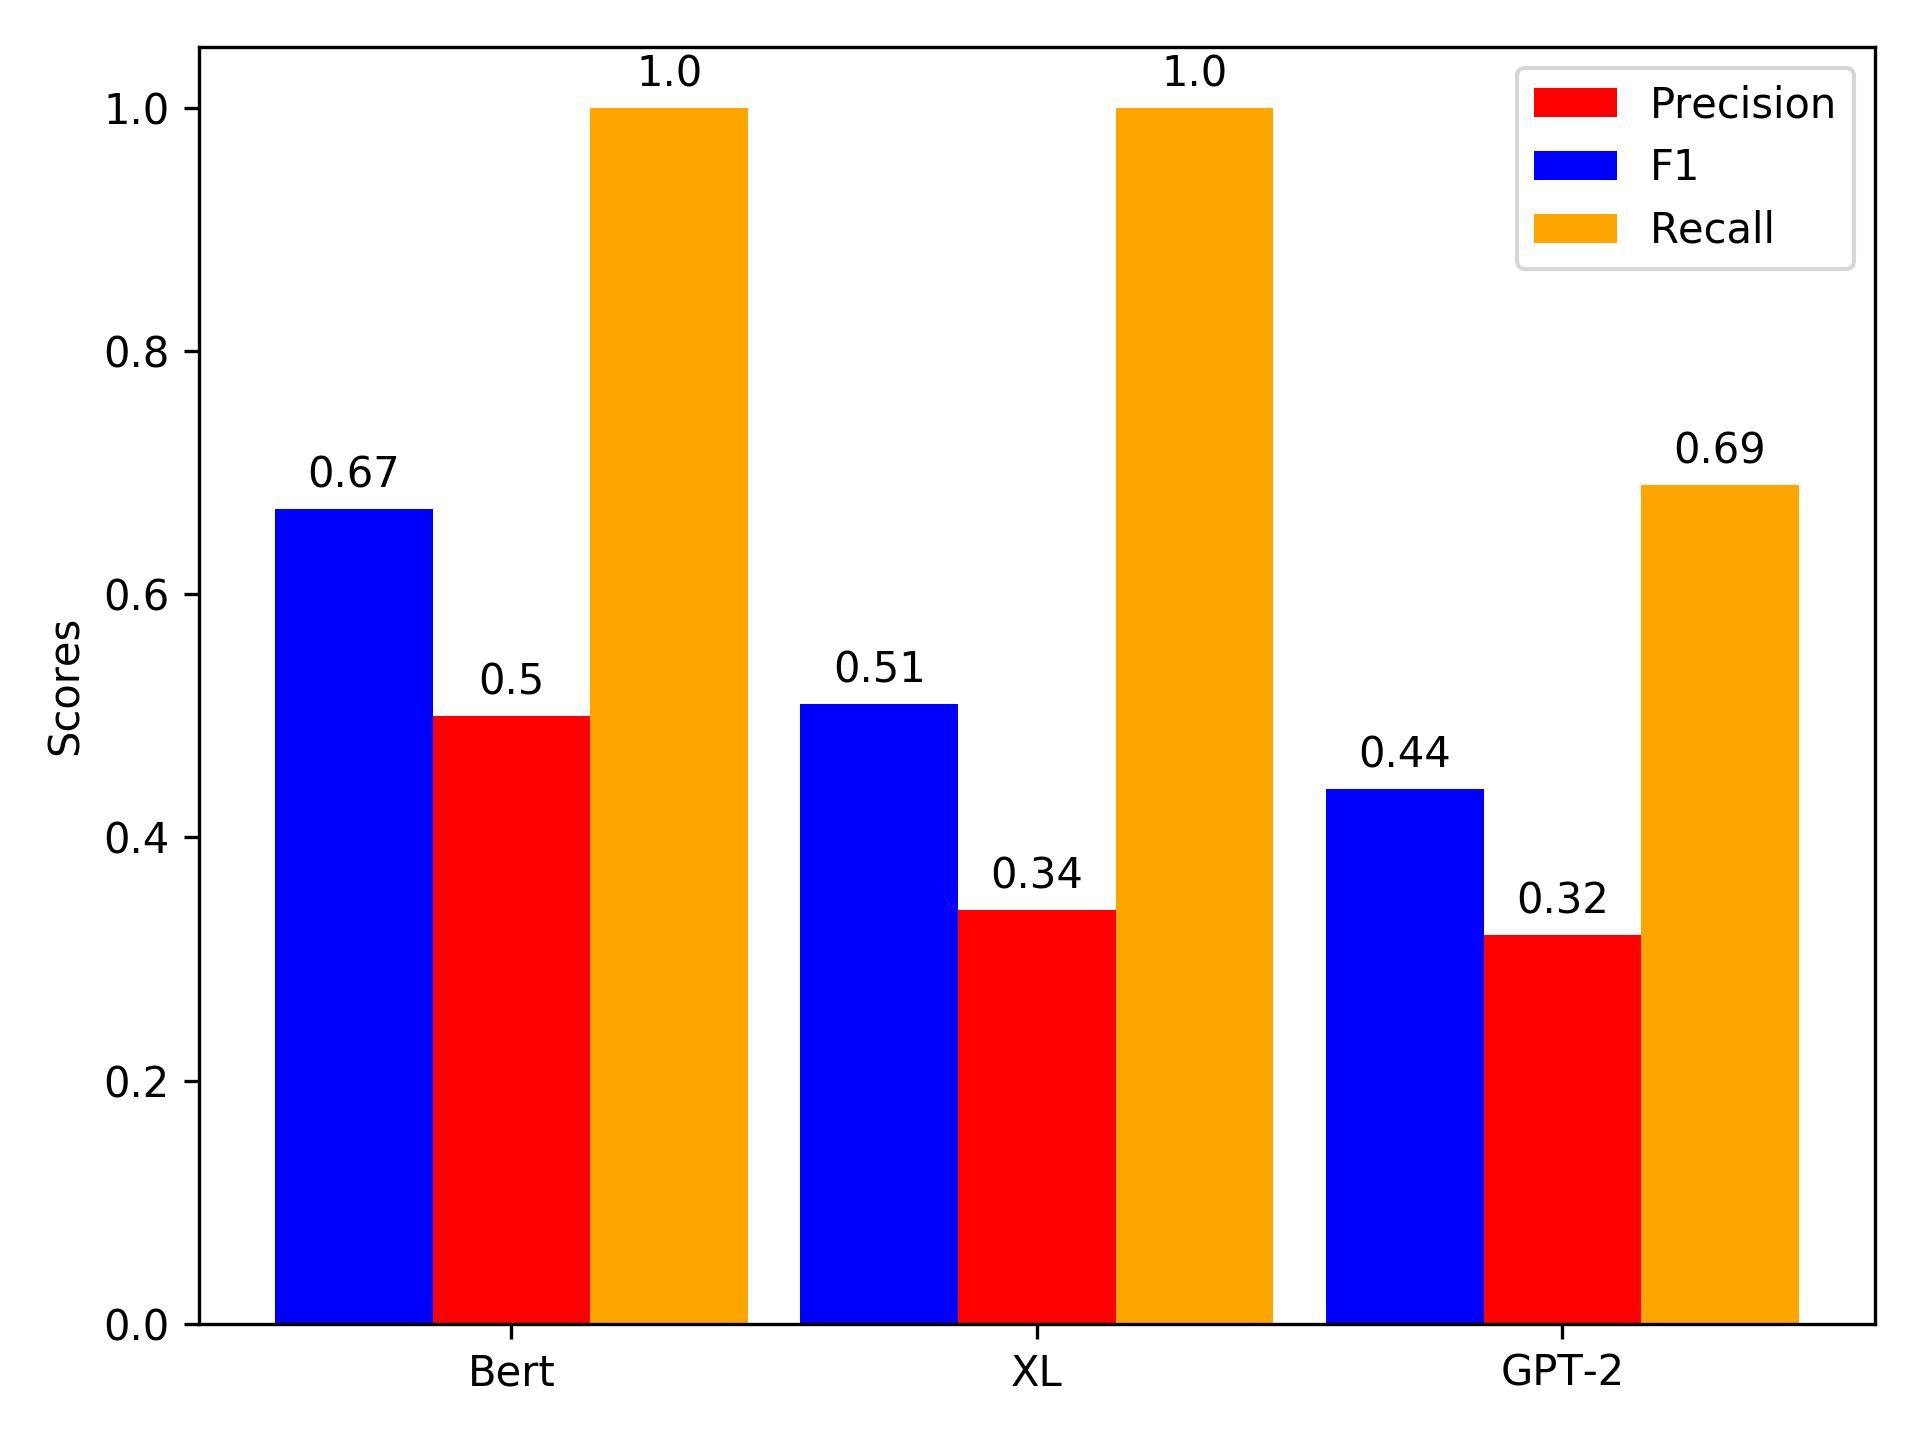
\includegraphics[trim={1cm 0.5cm 0cm 1cm}, width=0.322\textwidth]{results/average/multiclass_sequential_average_ratio_0.05.png}}
\hspace{\fill}
   \subfloat[10\% alteration\label{fig:results_multiclass_sequential_10} ]{%
      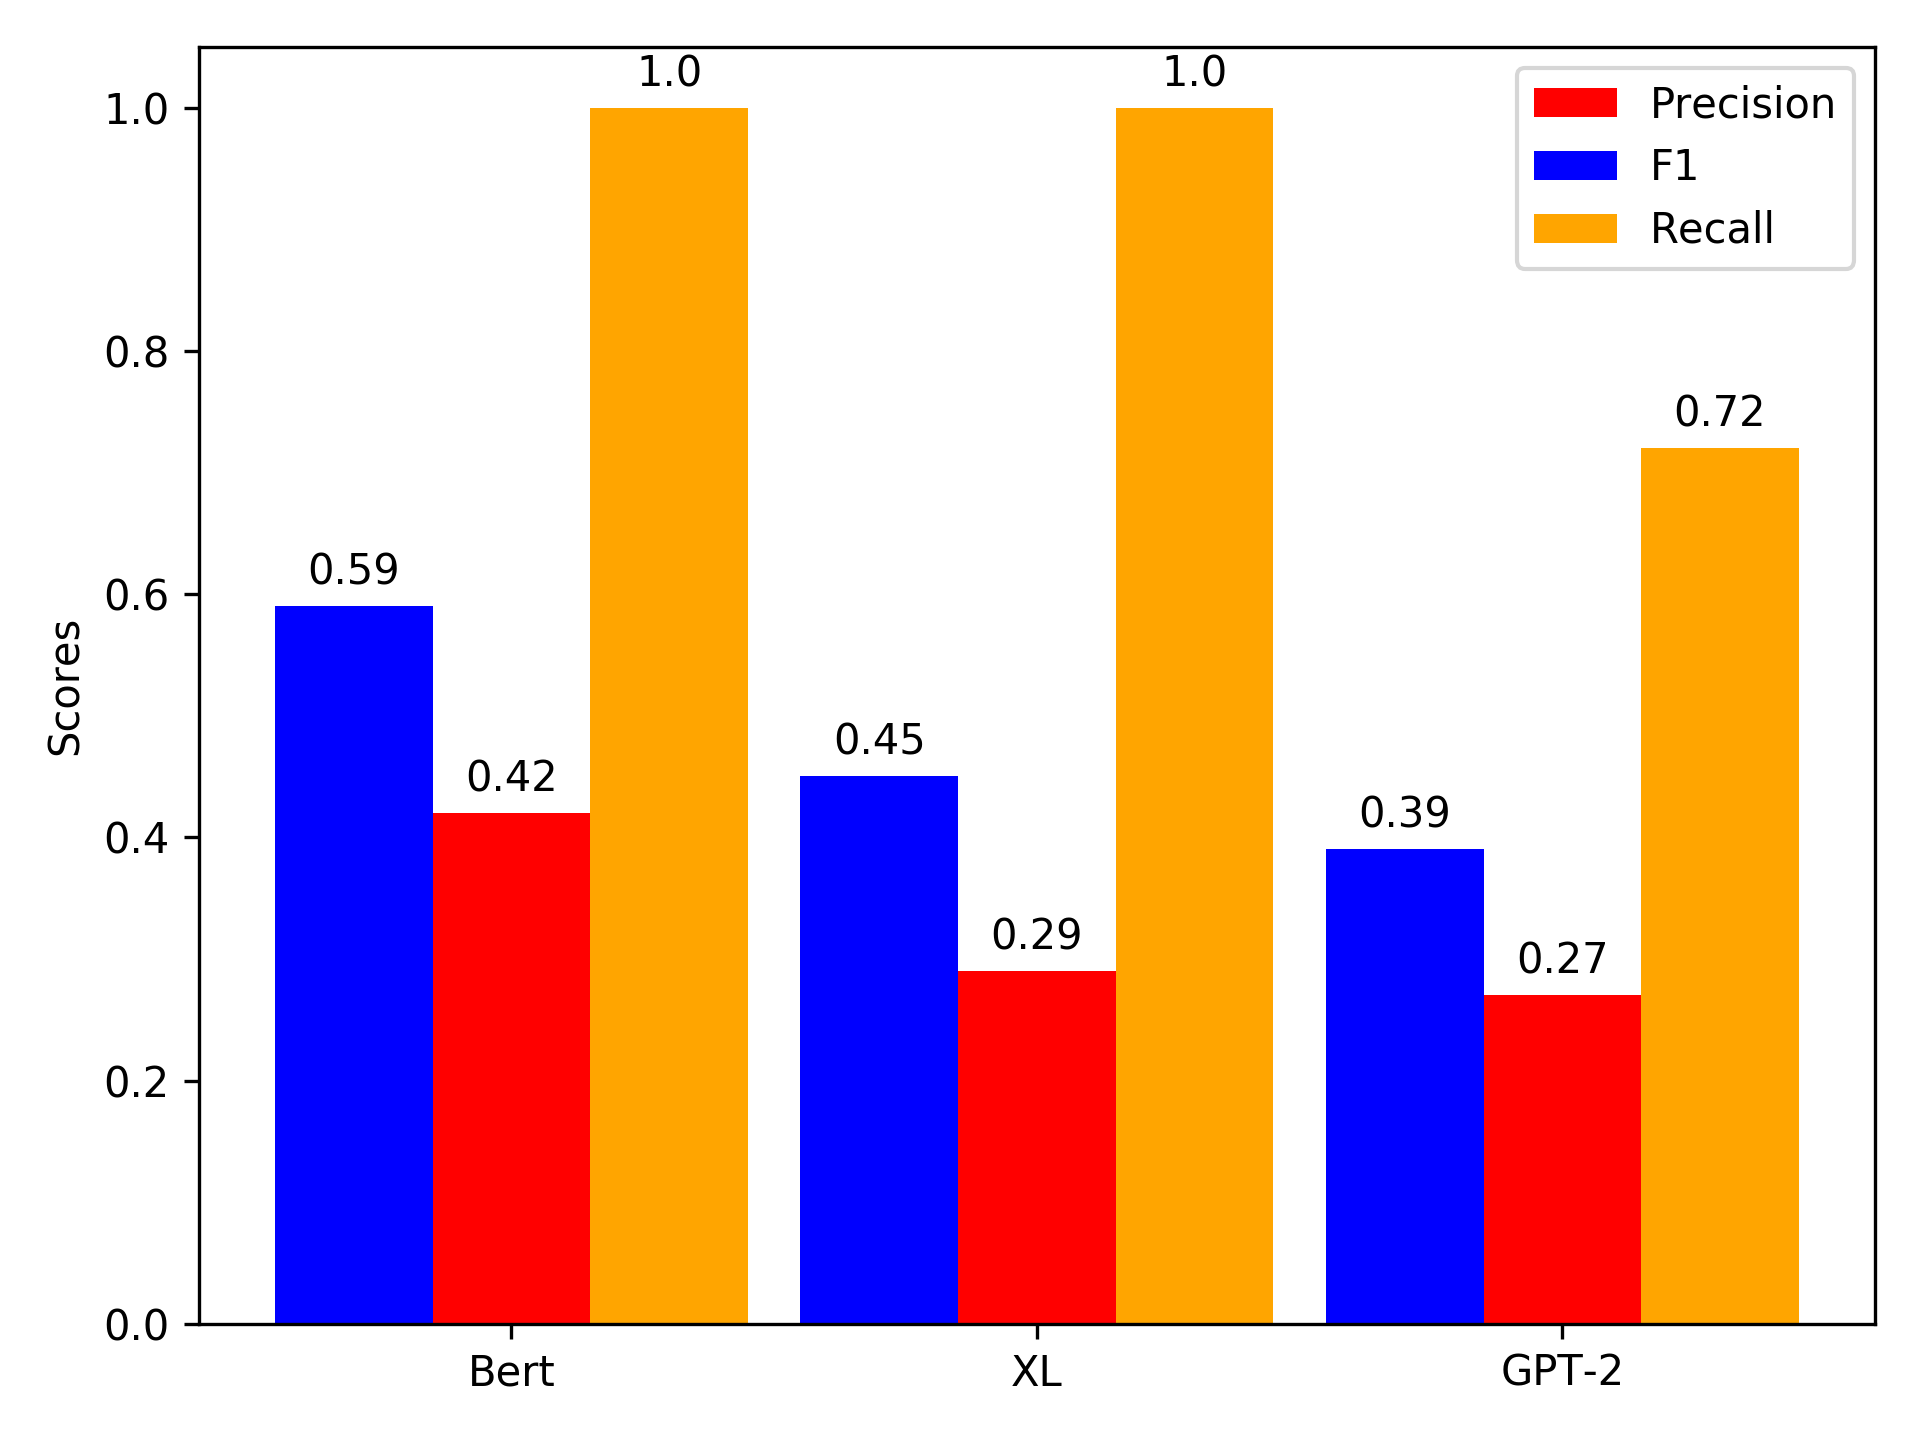
\includegraphics[trim={1cm 0.5cm 0cm 1cm}, width=0.322\textwidth]{results/average/multiclass_sequential_average_ratio_0.10.png}}
\hspace{\fill}
   \subfloat[15\% alteration\label{fig:results_multiclass_sequential_15}]{%
      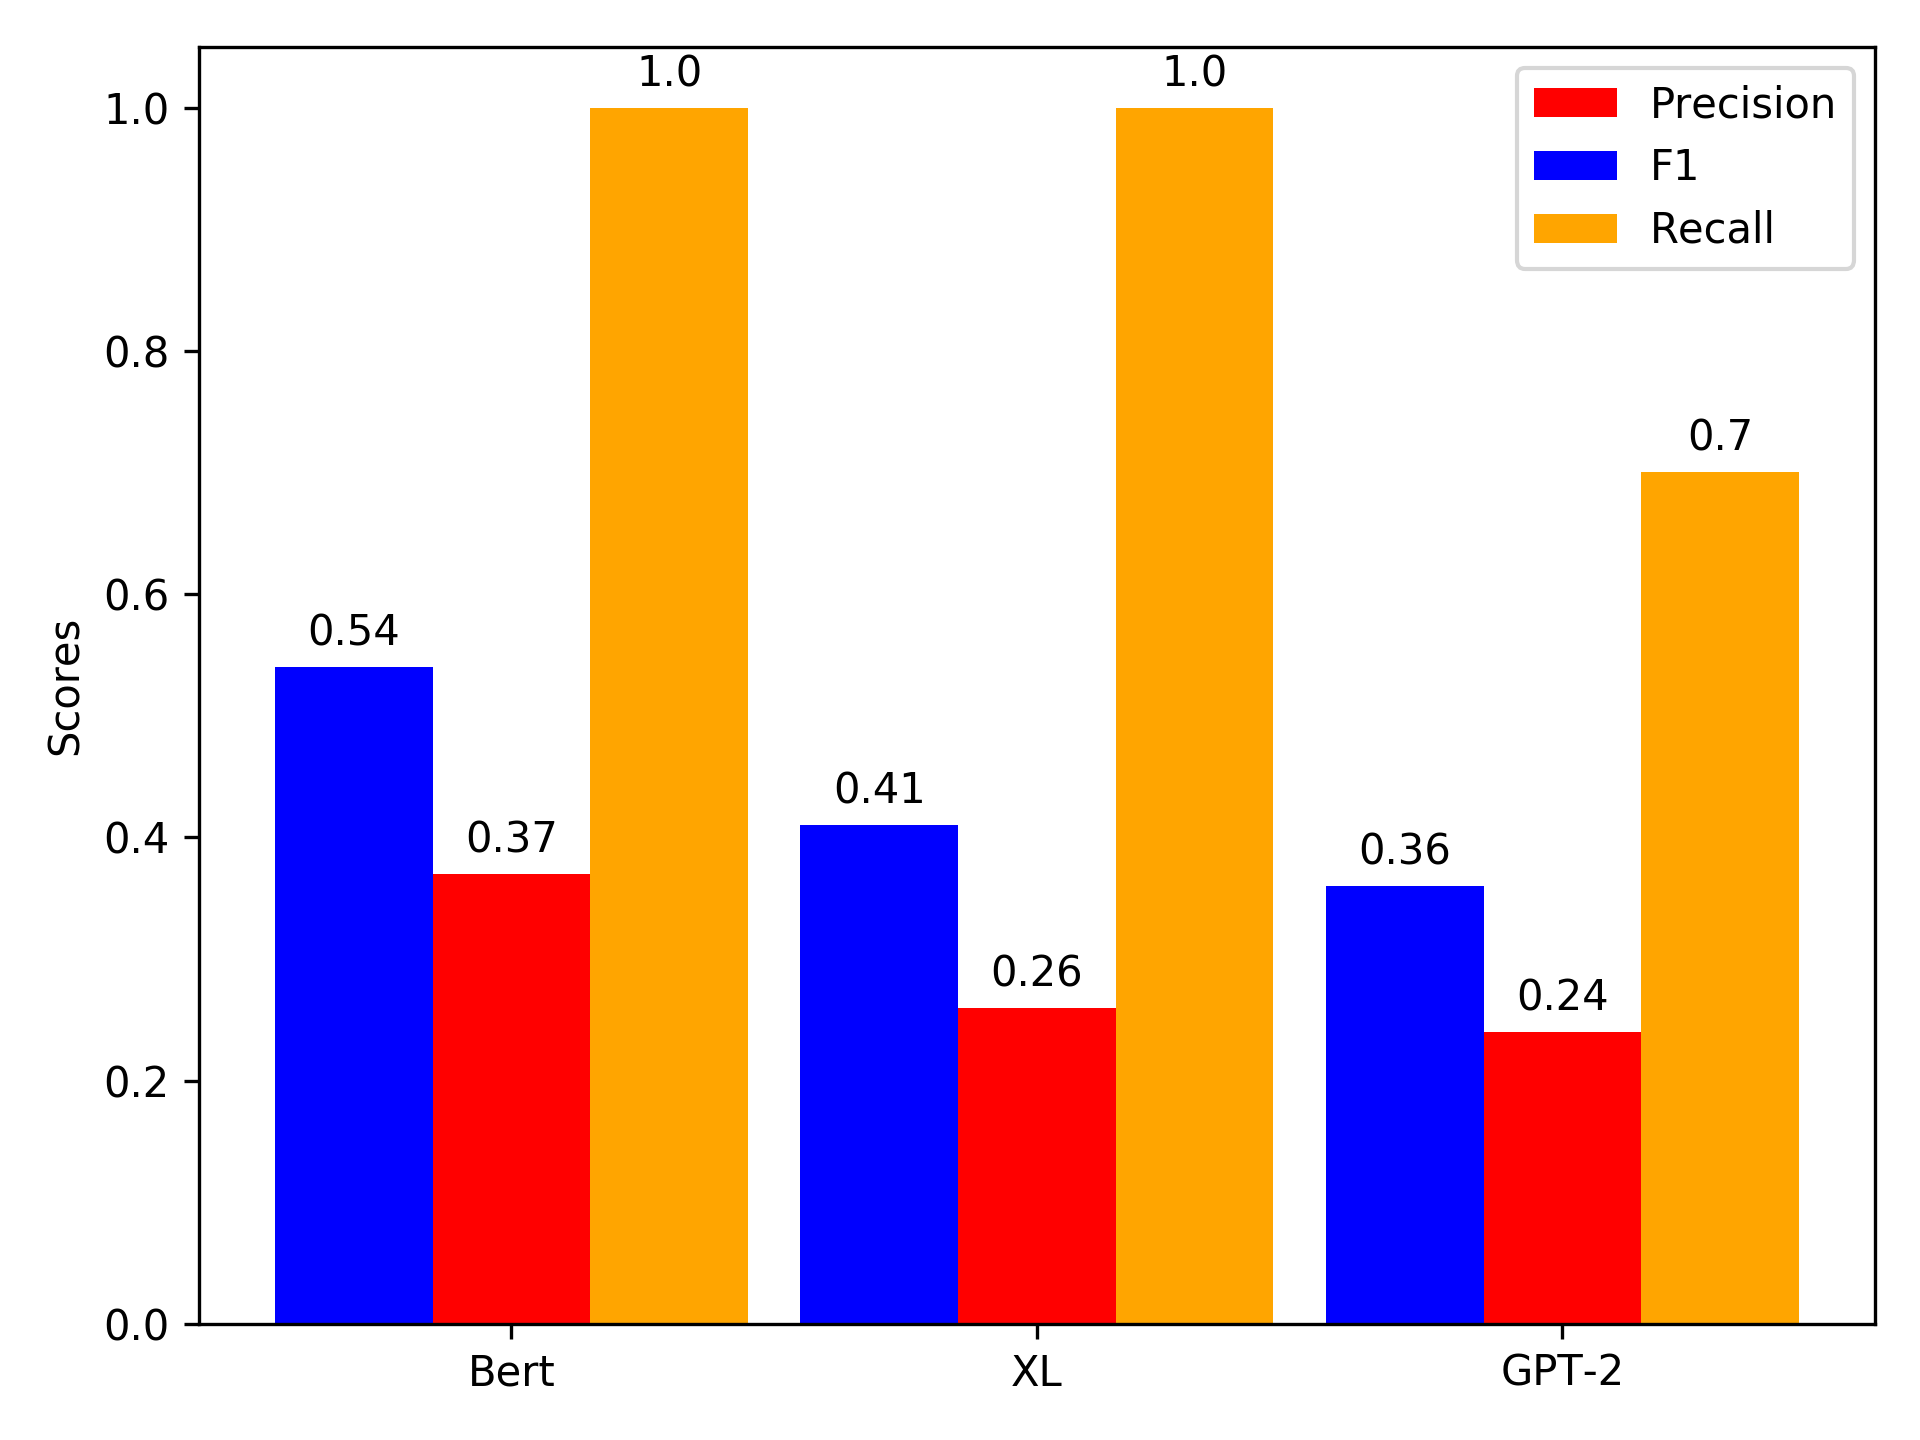
\includegraphics[trim={1cm 0.5cm 0cm 1cm}, width=0.322\textwidth]{results/average/multiclass_sequential_average_ratio_0.15.png}}\\
\caption{\label{fig:results_multiclass_sequential}Altering the order of log sequences at different ratios, inject semantically different anomalies, using classification.}
\end{figure*}

%multiclass qualitative
\begin{figure*}[ht!]
  \centering
  \captionsetup{justification=centering}
   \subfloat[5\% alteration\label{fig:results_multiclass_qualitative_5}]{%
      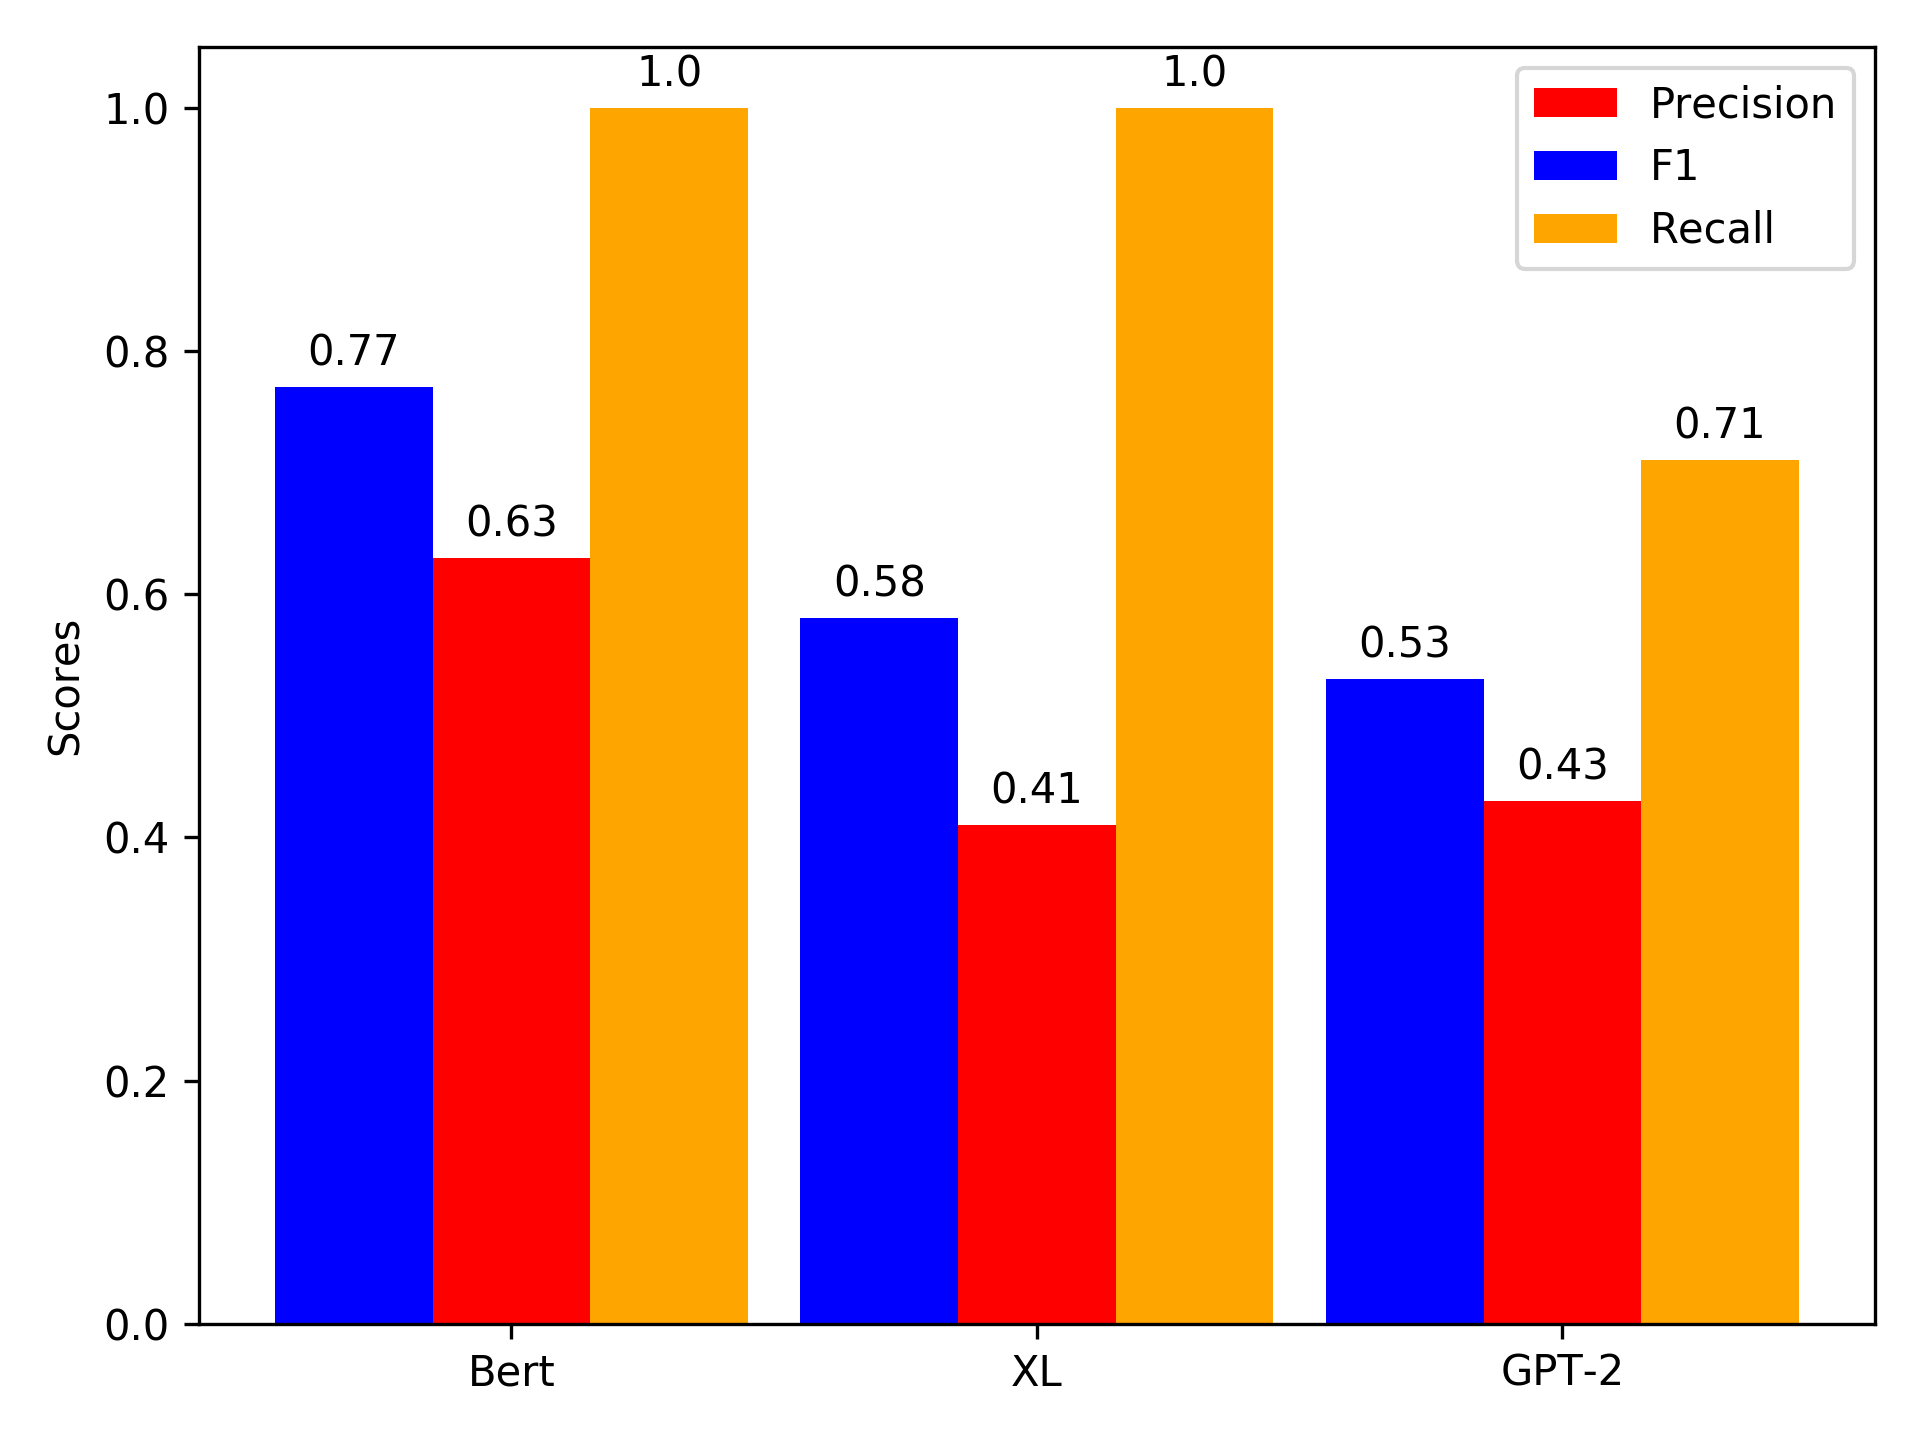
\includegraphics[trim={1cm 0.5cm 0cm 1cm}, width=0.322\textwidth]{results/average/multiclass_qualitative_average_ratio_0.05.png}}
\hspace{\fill}
   \subfloat[10\% alteration\label{fig:results_multiclass_qualitative_10} ]{%
      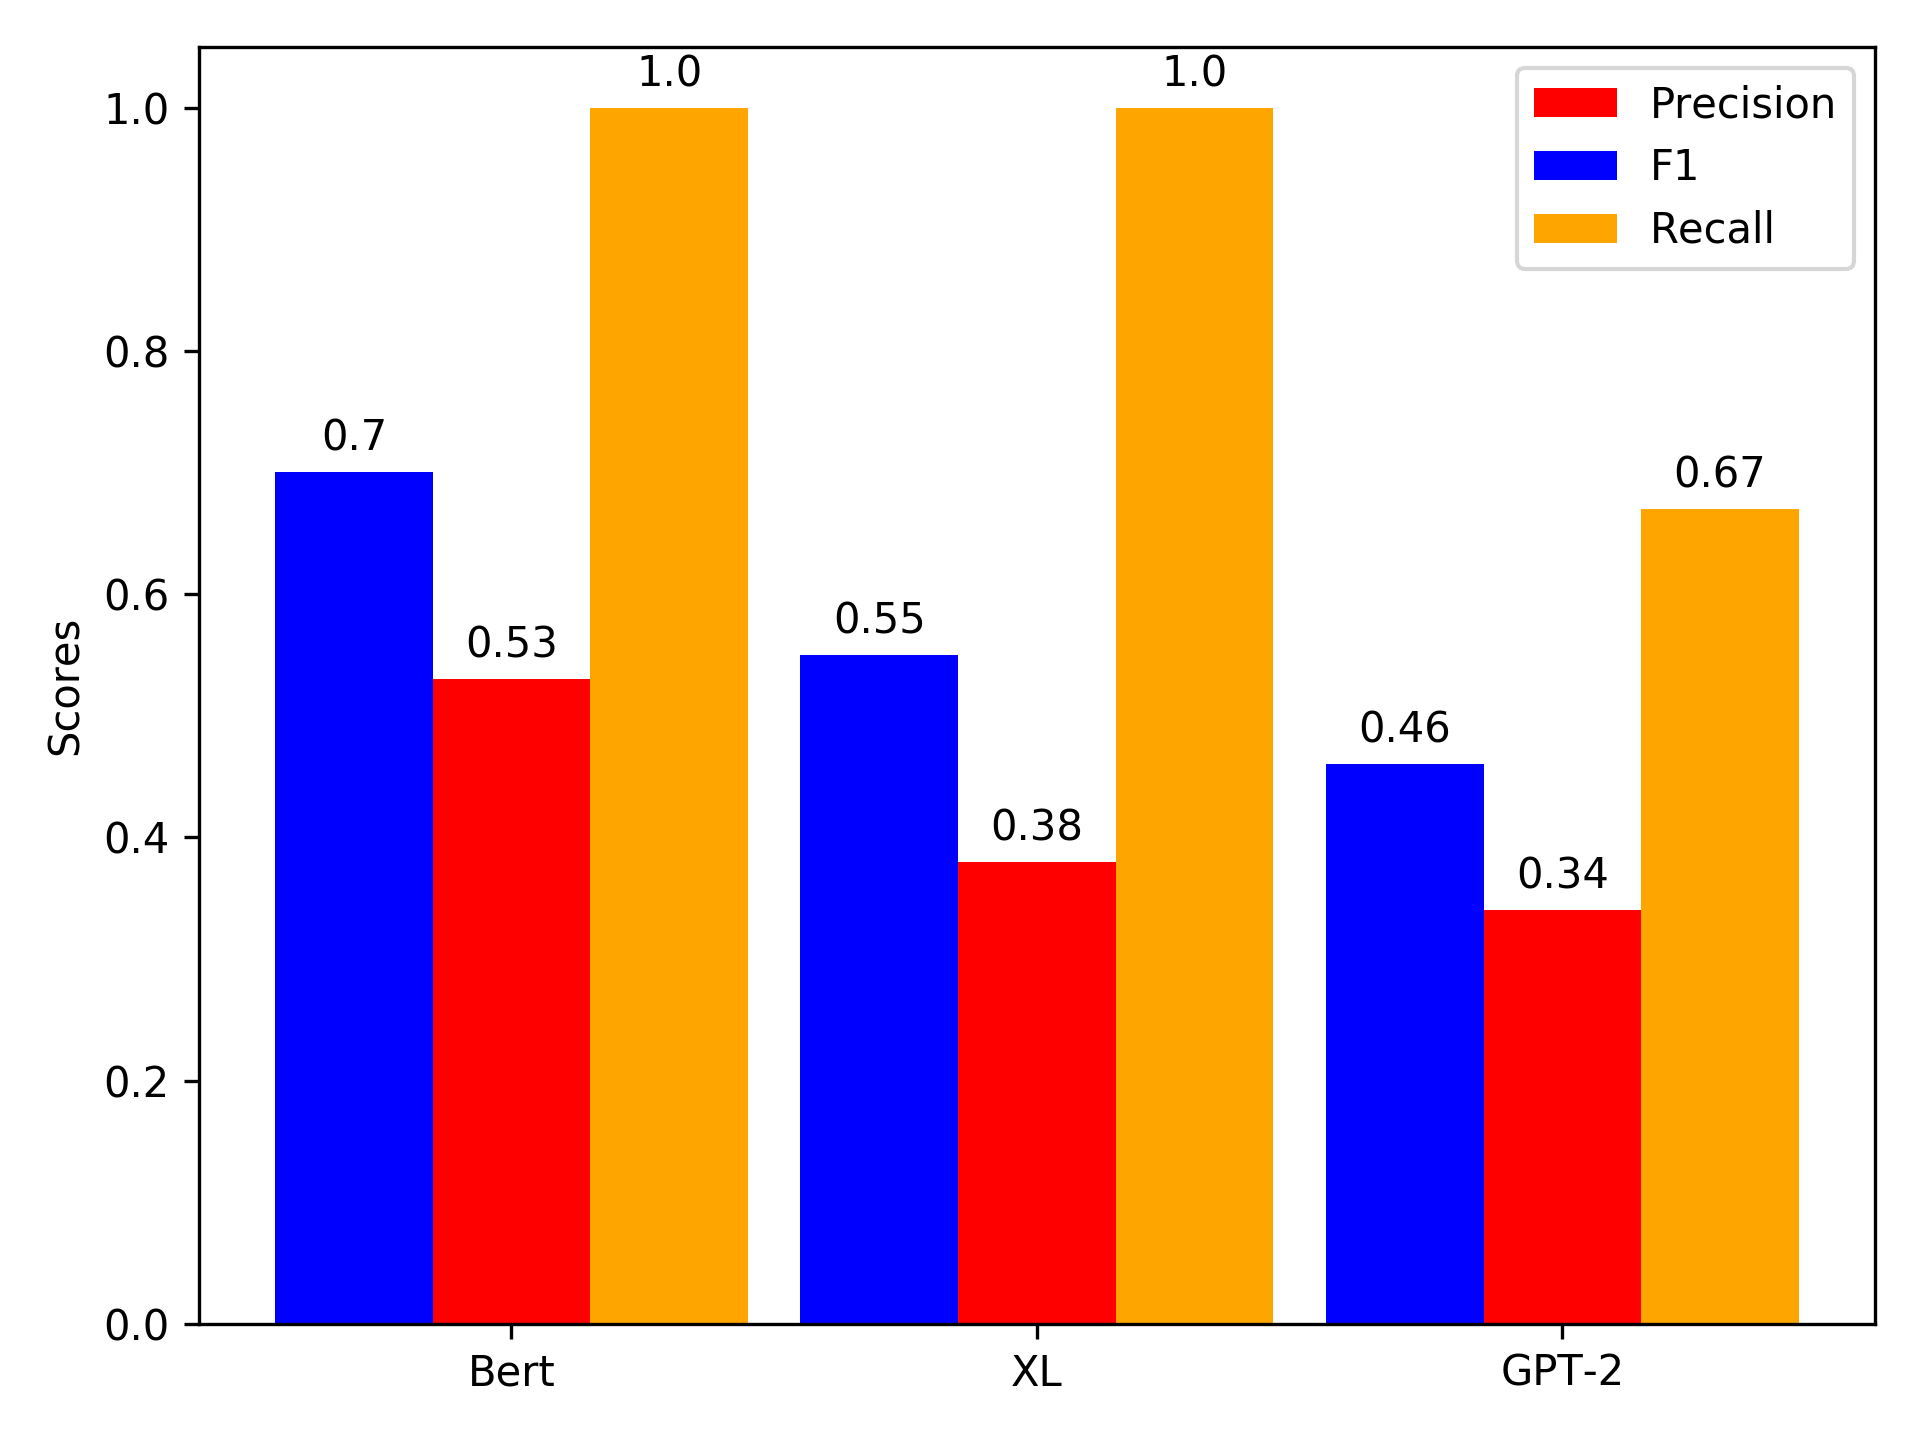
\includegraphics[trim={1cm 0.5cm 0cm 1cm}, width=0.322\textwidth]{results/average/multiclass_qualitative_average_ratio_0.10.png}}
\hspace{\fill}
   \subfloat[15\% alteration\label{fig:results_multiclass_qualitative_15}]{%
      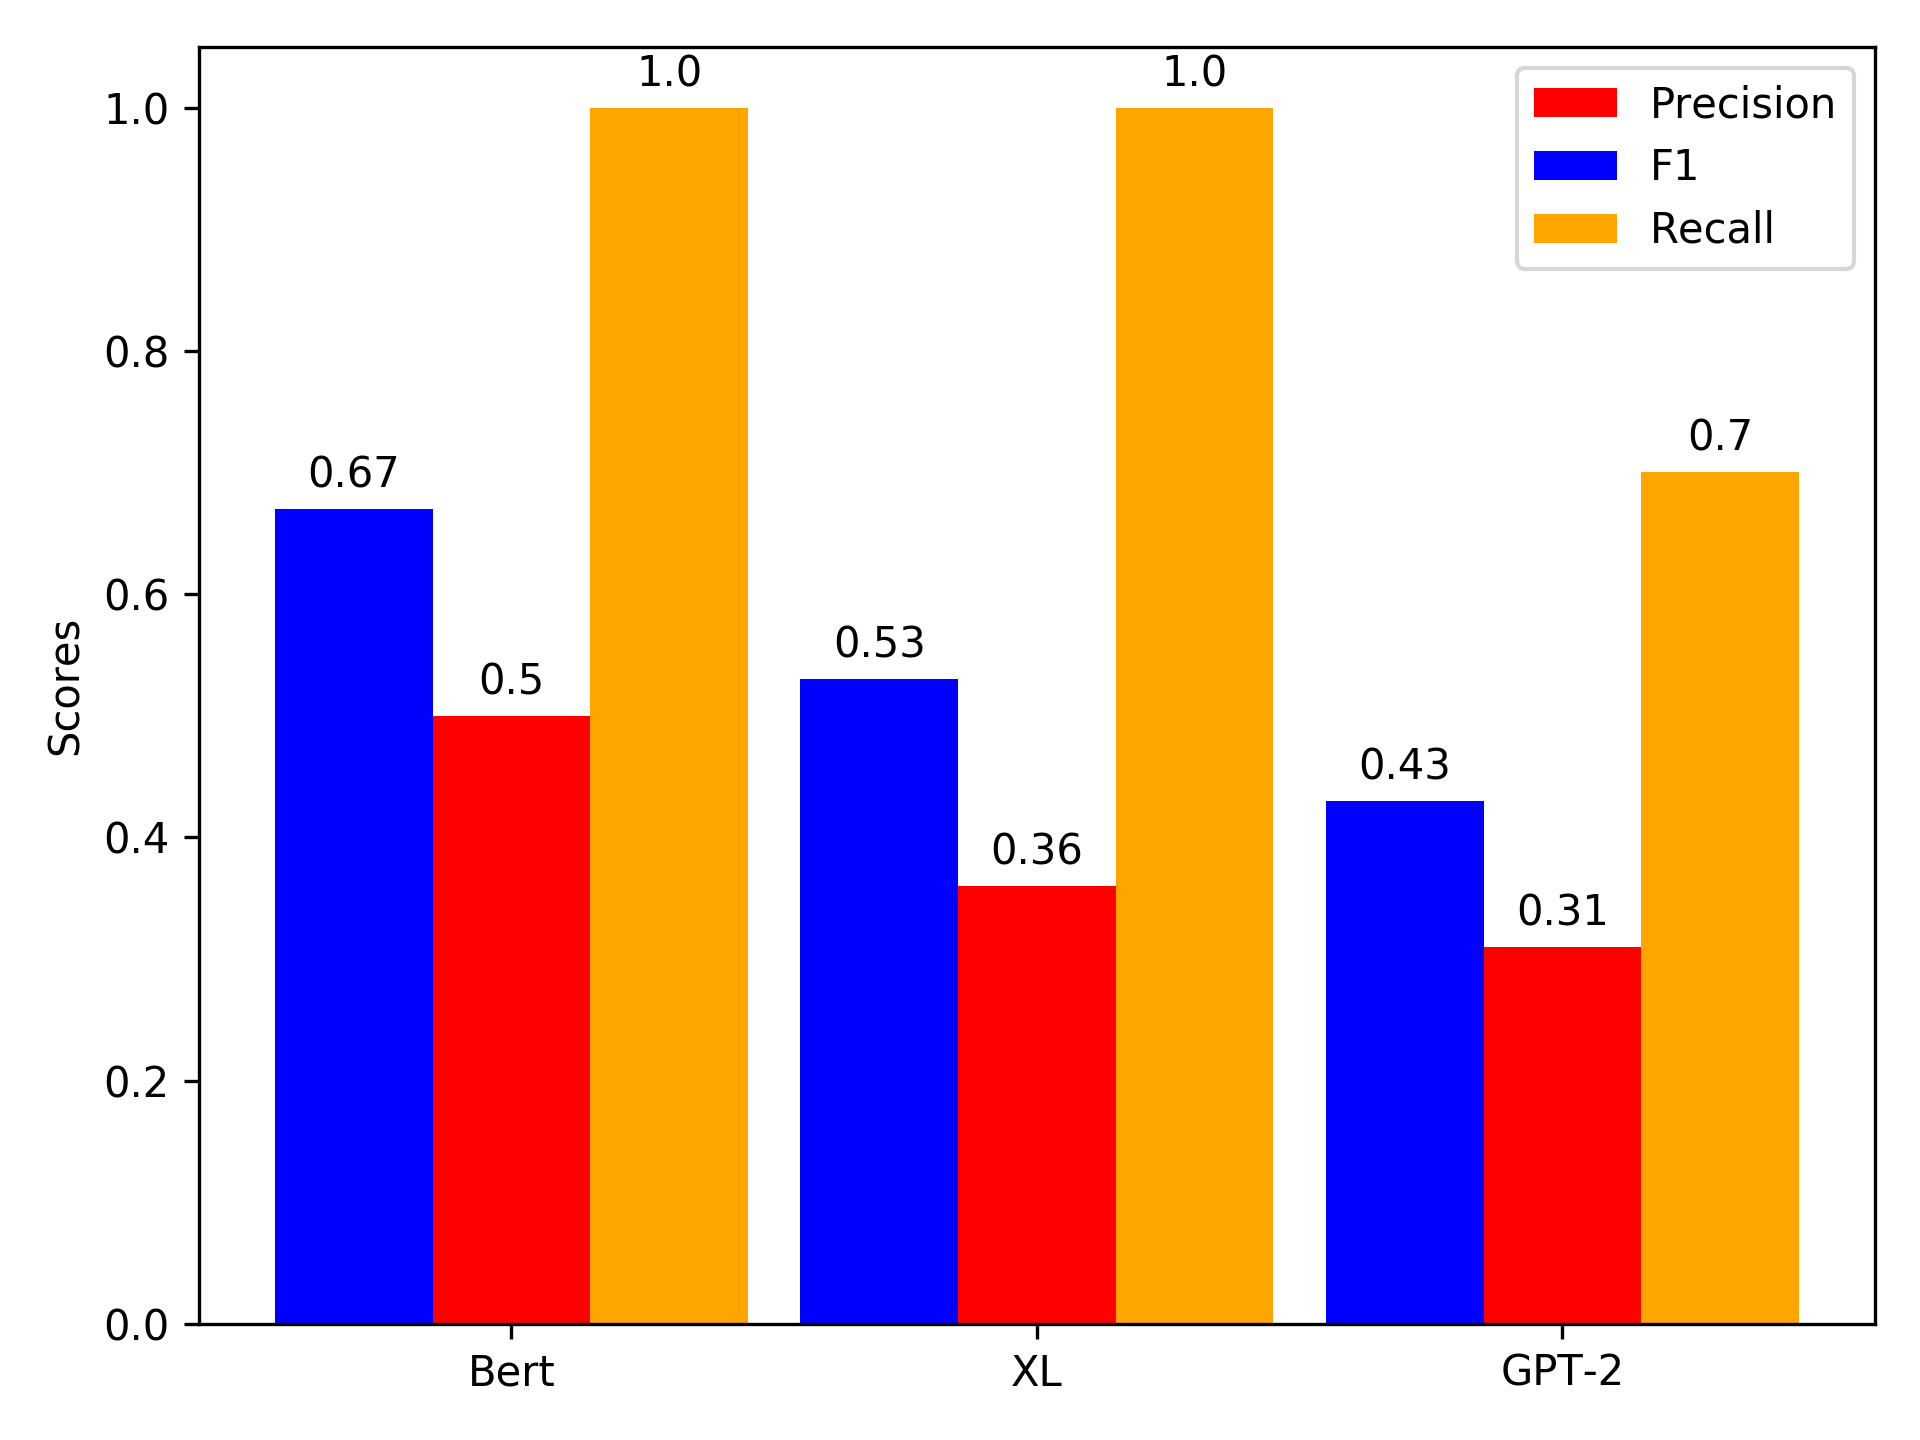
\includegraphics[trim={1cm 0.5cm 0cm 1cm}, width=0.322\textwidth]{results/average/multiclass_qualitative_average_ratio_0.15.png}}\\
\caption{\label{fig:results_multiclass_qualitative}Altering log events at different ratios, inject semantically different anomalies, using classification.}
\end{figure*}

\begin{figure}[H]
\centering
  \captionsetup{justification=centering}
  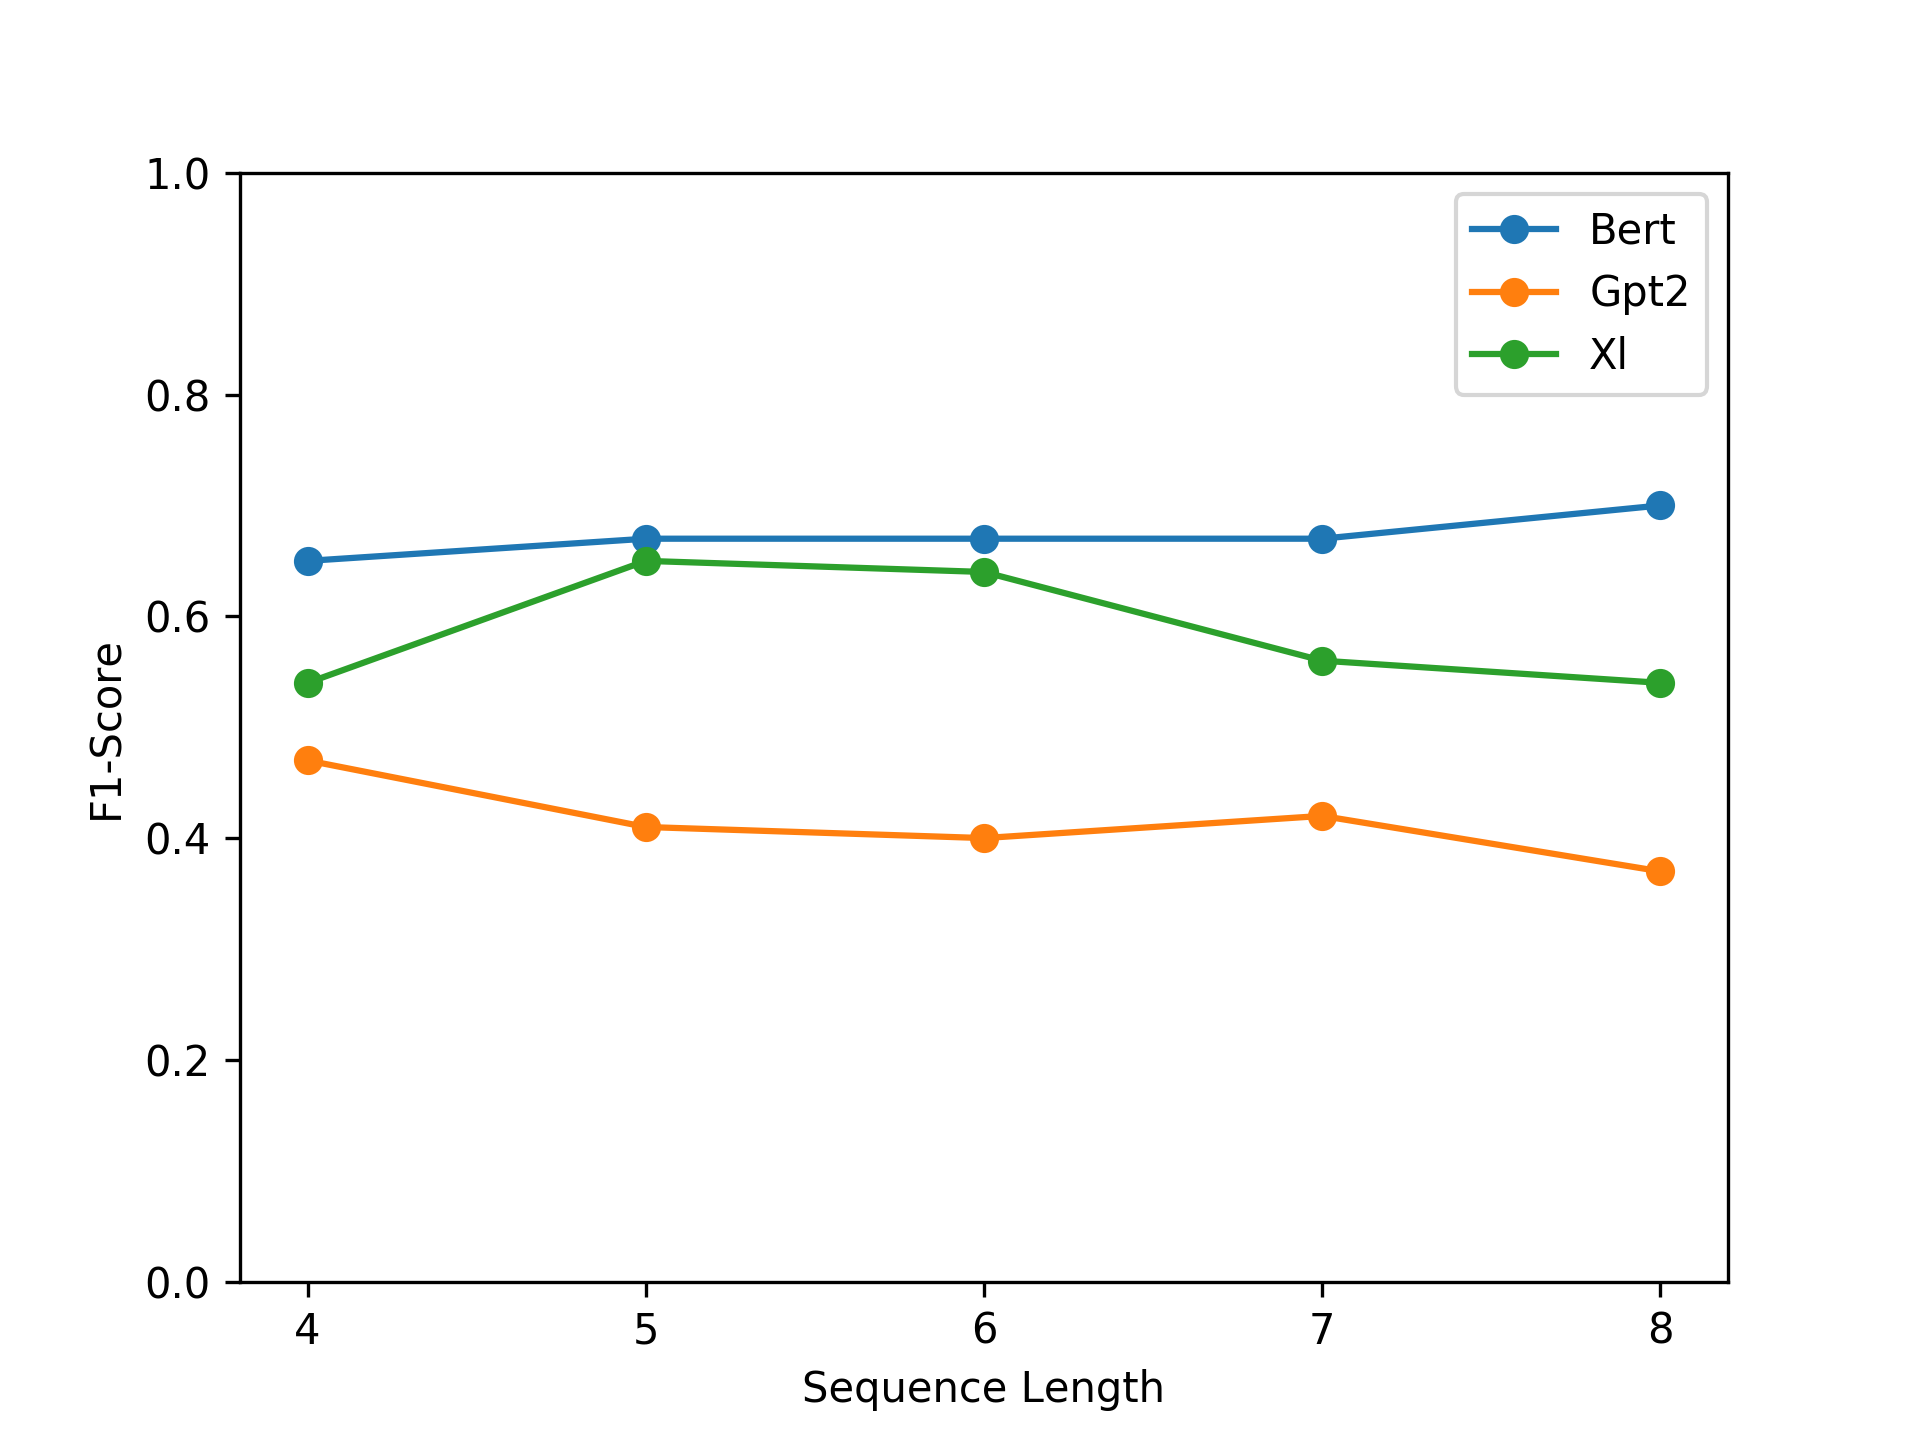
\includegraphics[width=7.7cm]{results/seq_len/sequence_len_classification.png}\\
  \caption{F1-Score for varying input sequence lengths, for 15\% of the log lines insert one word as alteration, inject semantically different anomalies, using classification.}
  \label{fig:seq_len_classification}
\end{figure}

\begin{figure}[H]
  \centering
  \captionsetup{justification=centering}
  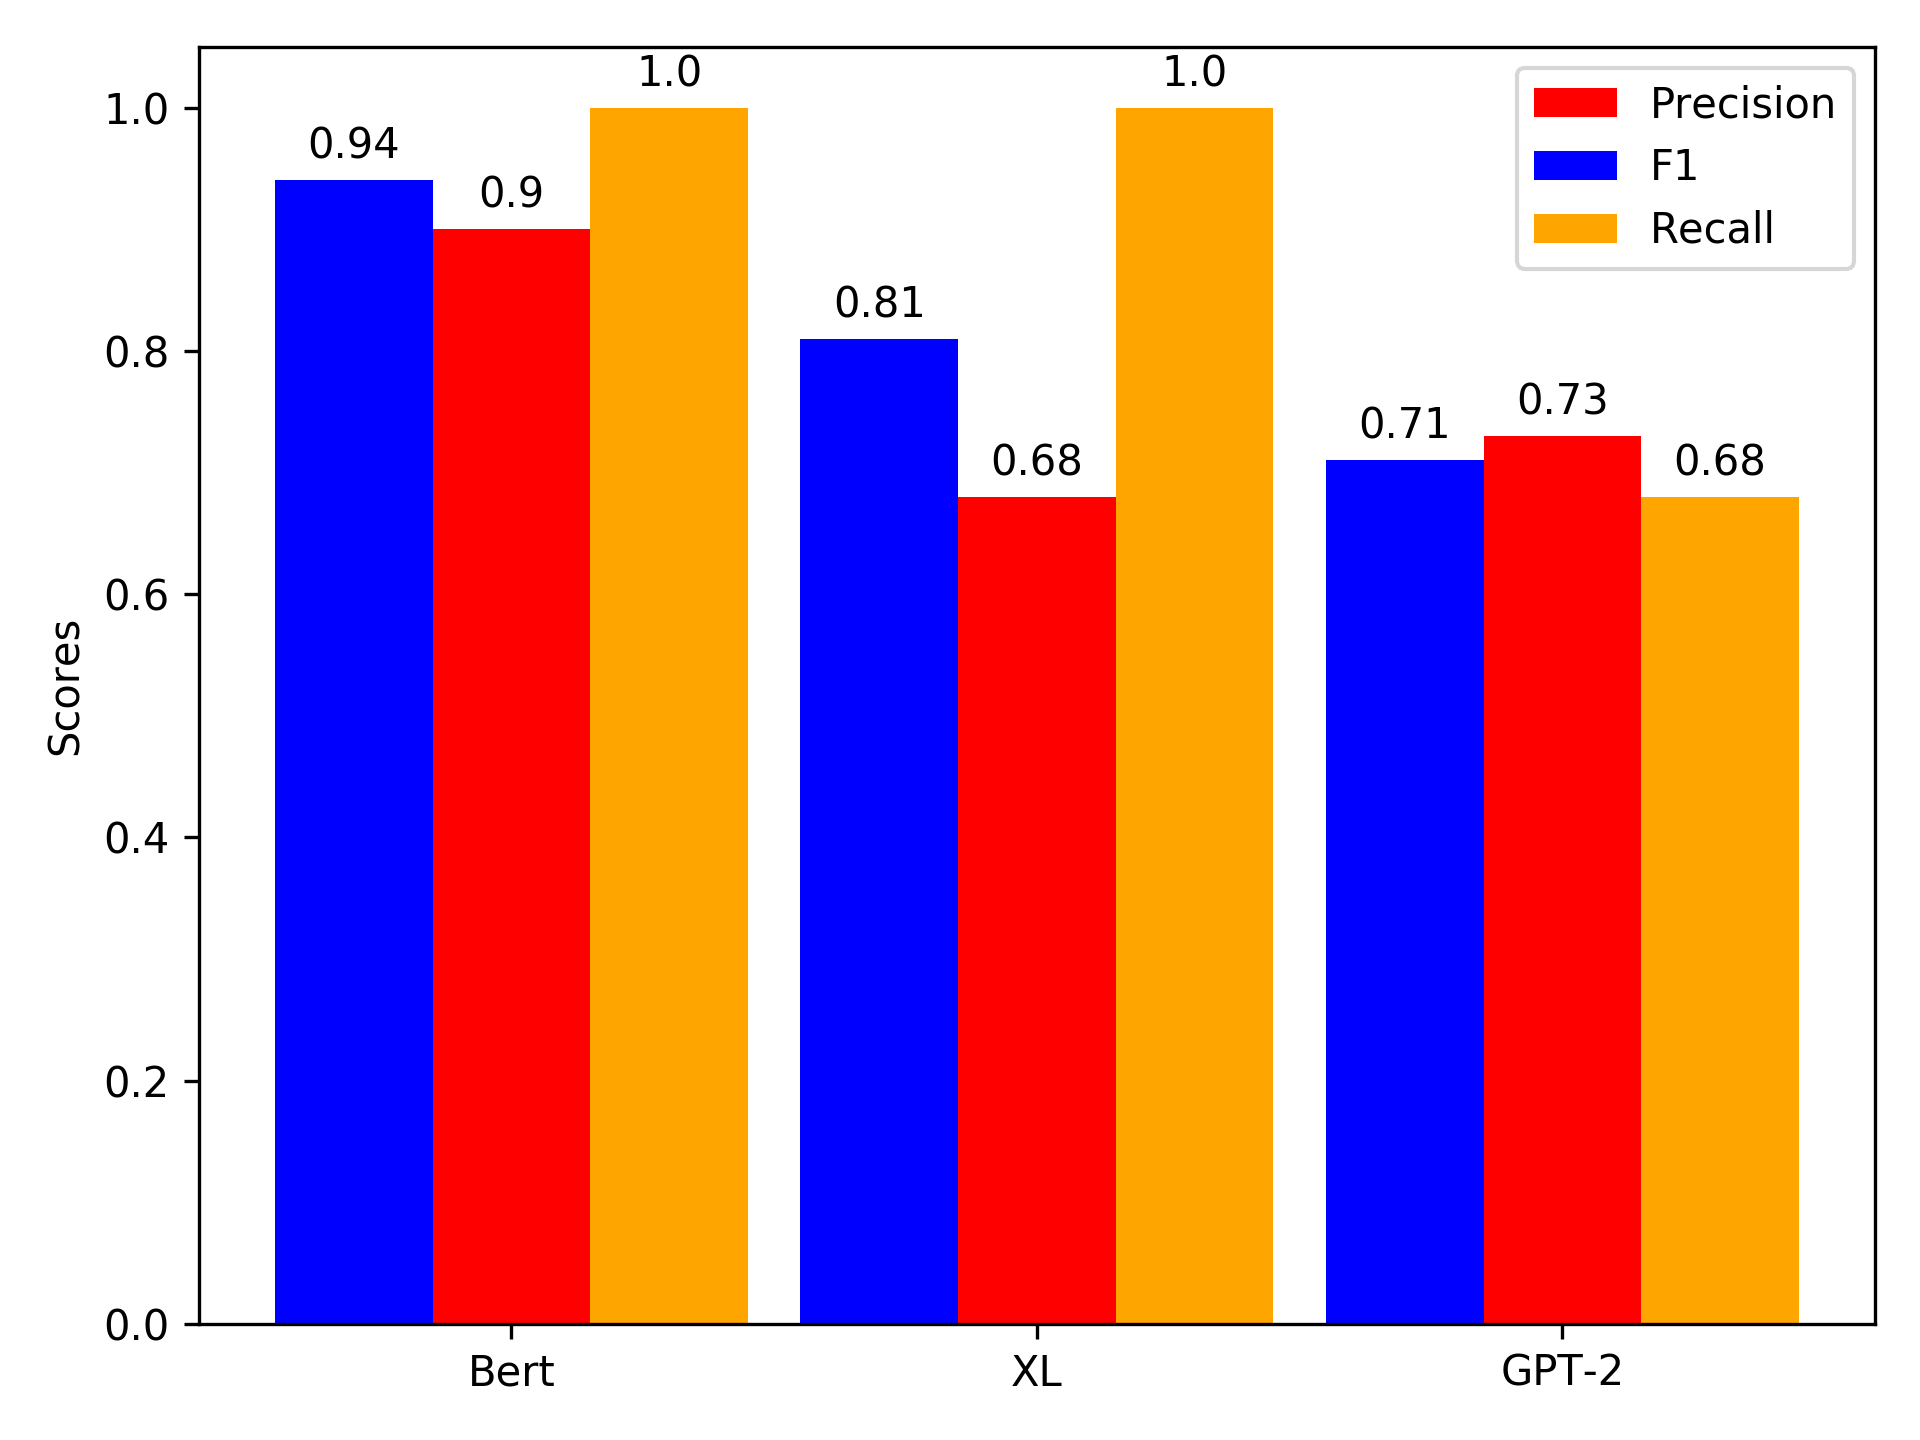
\includegraphics[width=8cm]{results/multiclass_replace_half.png}\\
  \caption{Inject semantically similar anomalies, using classification.}
  \label{fig:replace_words_classification}
\end{figure}


% multiclass sequence length



%%%%%
%%%%%
%%%%%

%%%%%%% TRANSFER LEARNING
%\subsection{Transfer Learning\label{sec:results_transfer}}
%In this subsection, the results of the transfer learning experiment are presented, using the classification-based approach in \ref{sec:results-classification-transfer} and the regression-based approach in \ref{sec:results-regression-transfer}.

\clearpage
\subsection{Transfer of Knowledge Using Regression \label{sec:results-regression-transfer}}

As described in \ref{sec:transfer_learning_setup}, the alterations that were injected separately in the experiments on one dataset in the last section, are now injected all at once, in order to simulate a different dataset $A$. Figure \ref{fig:results_transfer_regression} shows the results for alterations on 5\%, 10\% and 15\% of the log lines of all alterations each at the same time and injection of semantically different anomalies after 60 epochs of training on the train dataset $A$ and 5 epochs of training on the train dataset $B$. 
Similar to the previous experiments using regression, both Bert and GPT-2 achieve perfect recall values of 1.0, while XL-Transformers only achieves around 0.49 for increasing injection ratios. With regards to F1-score and precision, GPT-2 performs far better than Bert and XL-Transformers, yet Bert achieves a good F1-score of 0.95 and precision of 0.9 for 5\% alteration ratios, but degrades substantially for 10\% and 15\% to around 0.67 in F1-score and around 0.5 in precision. XL-Transformers shows an F1-score of 0.41 for 5\% alterations, 0.34 for 10\% alterations and 0.26 for 15\% alterations, and precision of 0.33 for 5\% alterations, 0.28 for 10\% alterations and 0.18 for 15\% alterations. GPT-2 shows very stable results, even with increasing ratio of injection. With a F1-score of 0.96 for 5\% alterations, 0.98 for 10\% alterations and 0.97 for 15\% alterations and precision of 0.92 for 5\% alterations, 0.95 for 10\% alterations and 0.94 for 15\% alterations and recall of 1.0, is ahead of the other two language models in every metric, except for recall, where Bert performs equally well. Bert performs second-best, while XL-Transformers achieves the least useful results.

Figure \ref{fig:results_transfer_regression_per_epoch} depicts the development of the metrics of detecting anomalies for every additional epoch of training on dataset $B$. It is clearly visible, that XL-Transformers improves the most per epoch, with an increase of the F1-score from 0.1 to 0.26 and recall from 0.17 to 0.47. Bert has a smaller increase per training epoch, with F1-score increasing from 0.62 to 0.68, while recall already starts at 1.0. The results of GPT-2 do not change significantly much per epoch for every metric, but start at a very high level already for every metric clearly above 0.9, corresponding to the findings already made on GPT-2 using regression in \ref{sec:results-regression}.

The results for injecting 5\% semantically similar anomalies for transfer of knowledge with 15\% alterations using regression can be seen in figure \ref{fig:replace_words_regression_transfer}. Similar results as in \ref{sec:results-regression} are yet again achieved, where GPT-2 proves to be robust in the previous experiment, it is not able to distinguish the semantically similar log lines from the normal ones well. Bert and XL-Transformers are able to achieve better results, with Bert achieving a F1-score of 0.63, 0.58 and recall of 0.7, XL-Transformers achieving a F1-score of 0.55 precision of 0.45 and recall of 0.7, GPT-2 is only able to achieve a F1-score of 0.08, precision of 0.23 and recall of 0.05. This proves again that Bert is able to execute the task of anomaly detection for transfer of knowledge using regression best overall, when both types of anomaly injections are considered.

\begin{comment}
\begin{figure}[h]
  \centering
  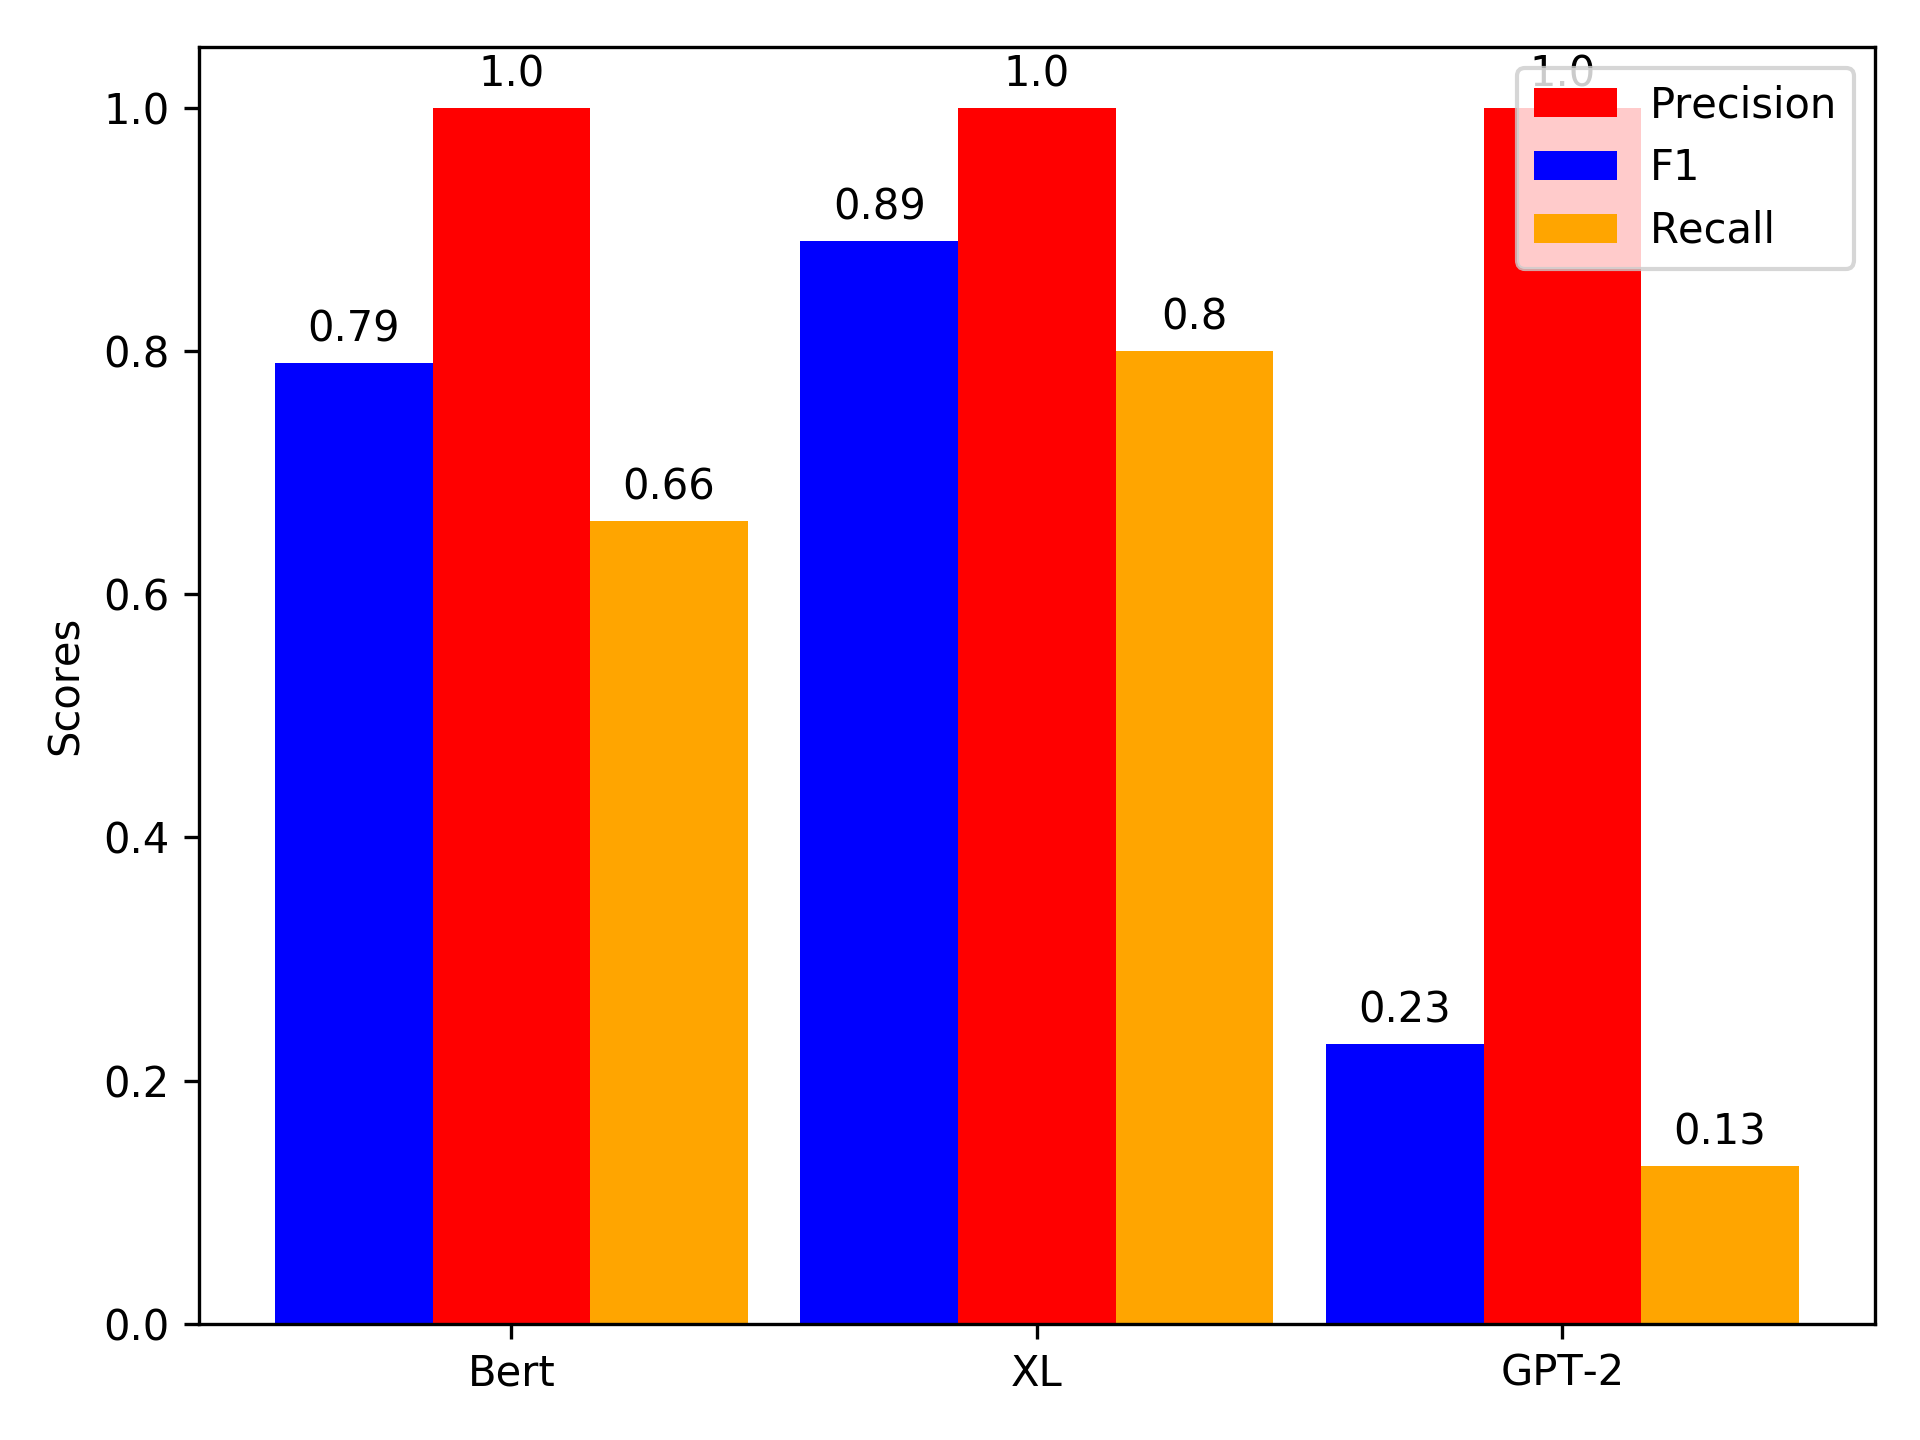
\includegraphics[width=6cm,height=4.5cm]{results/transfer/transfer_regression_reverse.png}\\
  \caption{Scores for detecting reversed order of log events for transfer learning, using regression.}
  \label{fig:regression_transfer_reverse}
\end{figure}
\end{comment}

\begin{figure*}[ht!]
  \centering
  \captionsetup{justification=centering}
   \subfloat[5\% alteration\label{fig:results_transfer_regression_0.05}]{%
      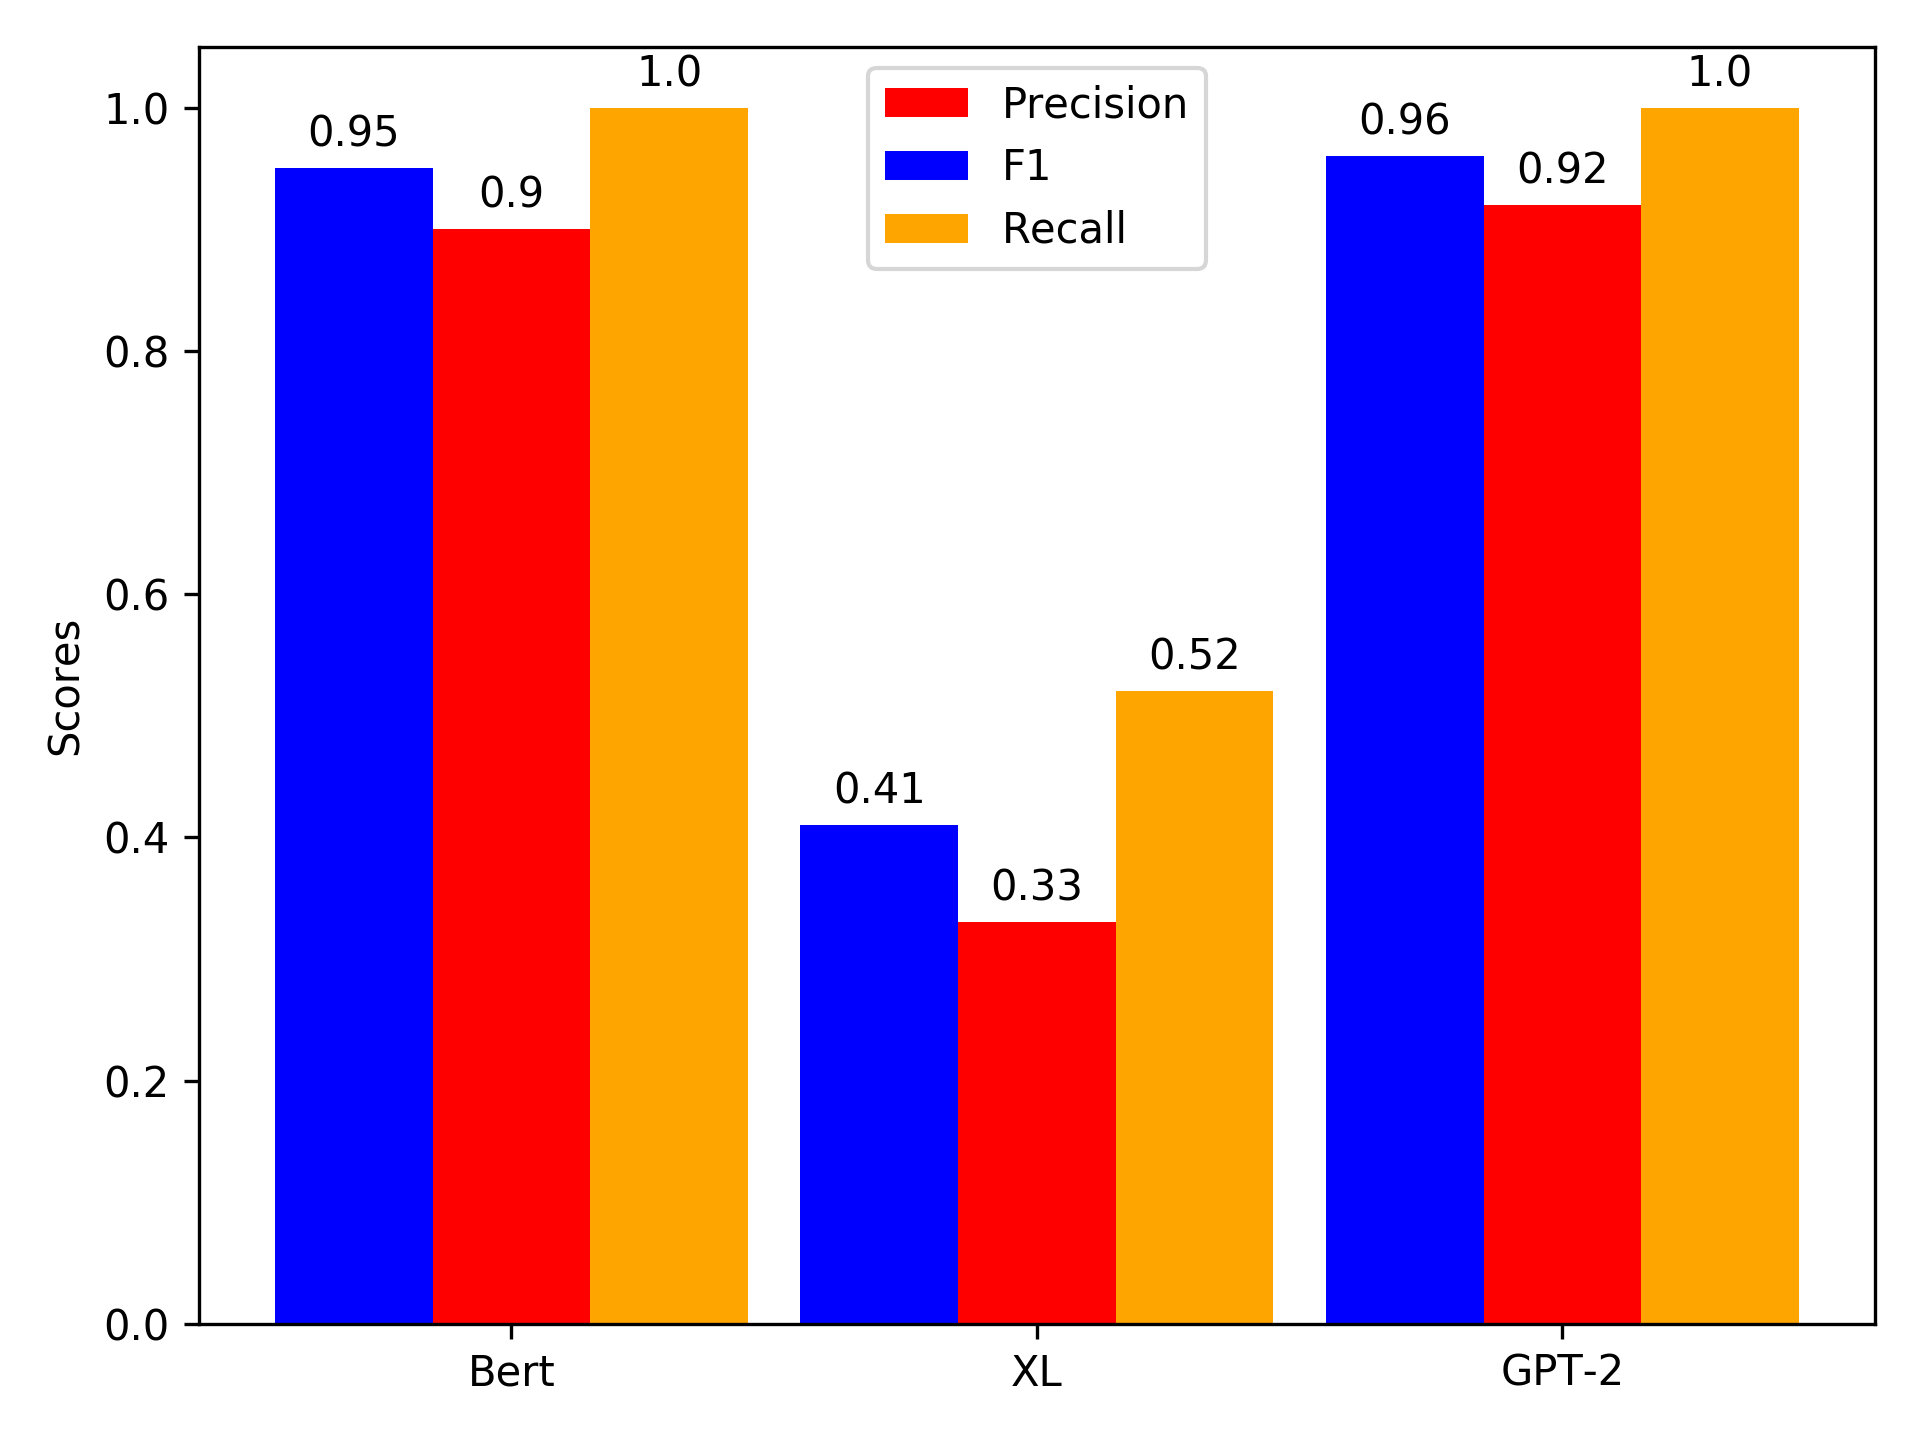
\includegraphics[trim={1cm 0.5cm 0cm 1cm}, width=0.322\textwidth]{results/transfer/transfer_regression_0.05_ratio.png}}
\hspace{\fill}
   \subfloat[10\% alteration\label{fig:results_transfer_regression_0.10} ]{%
      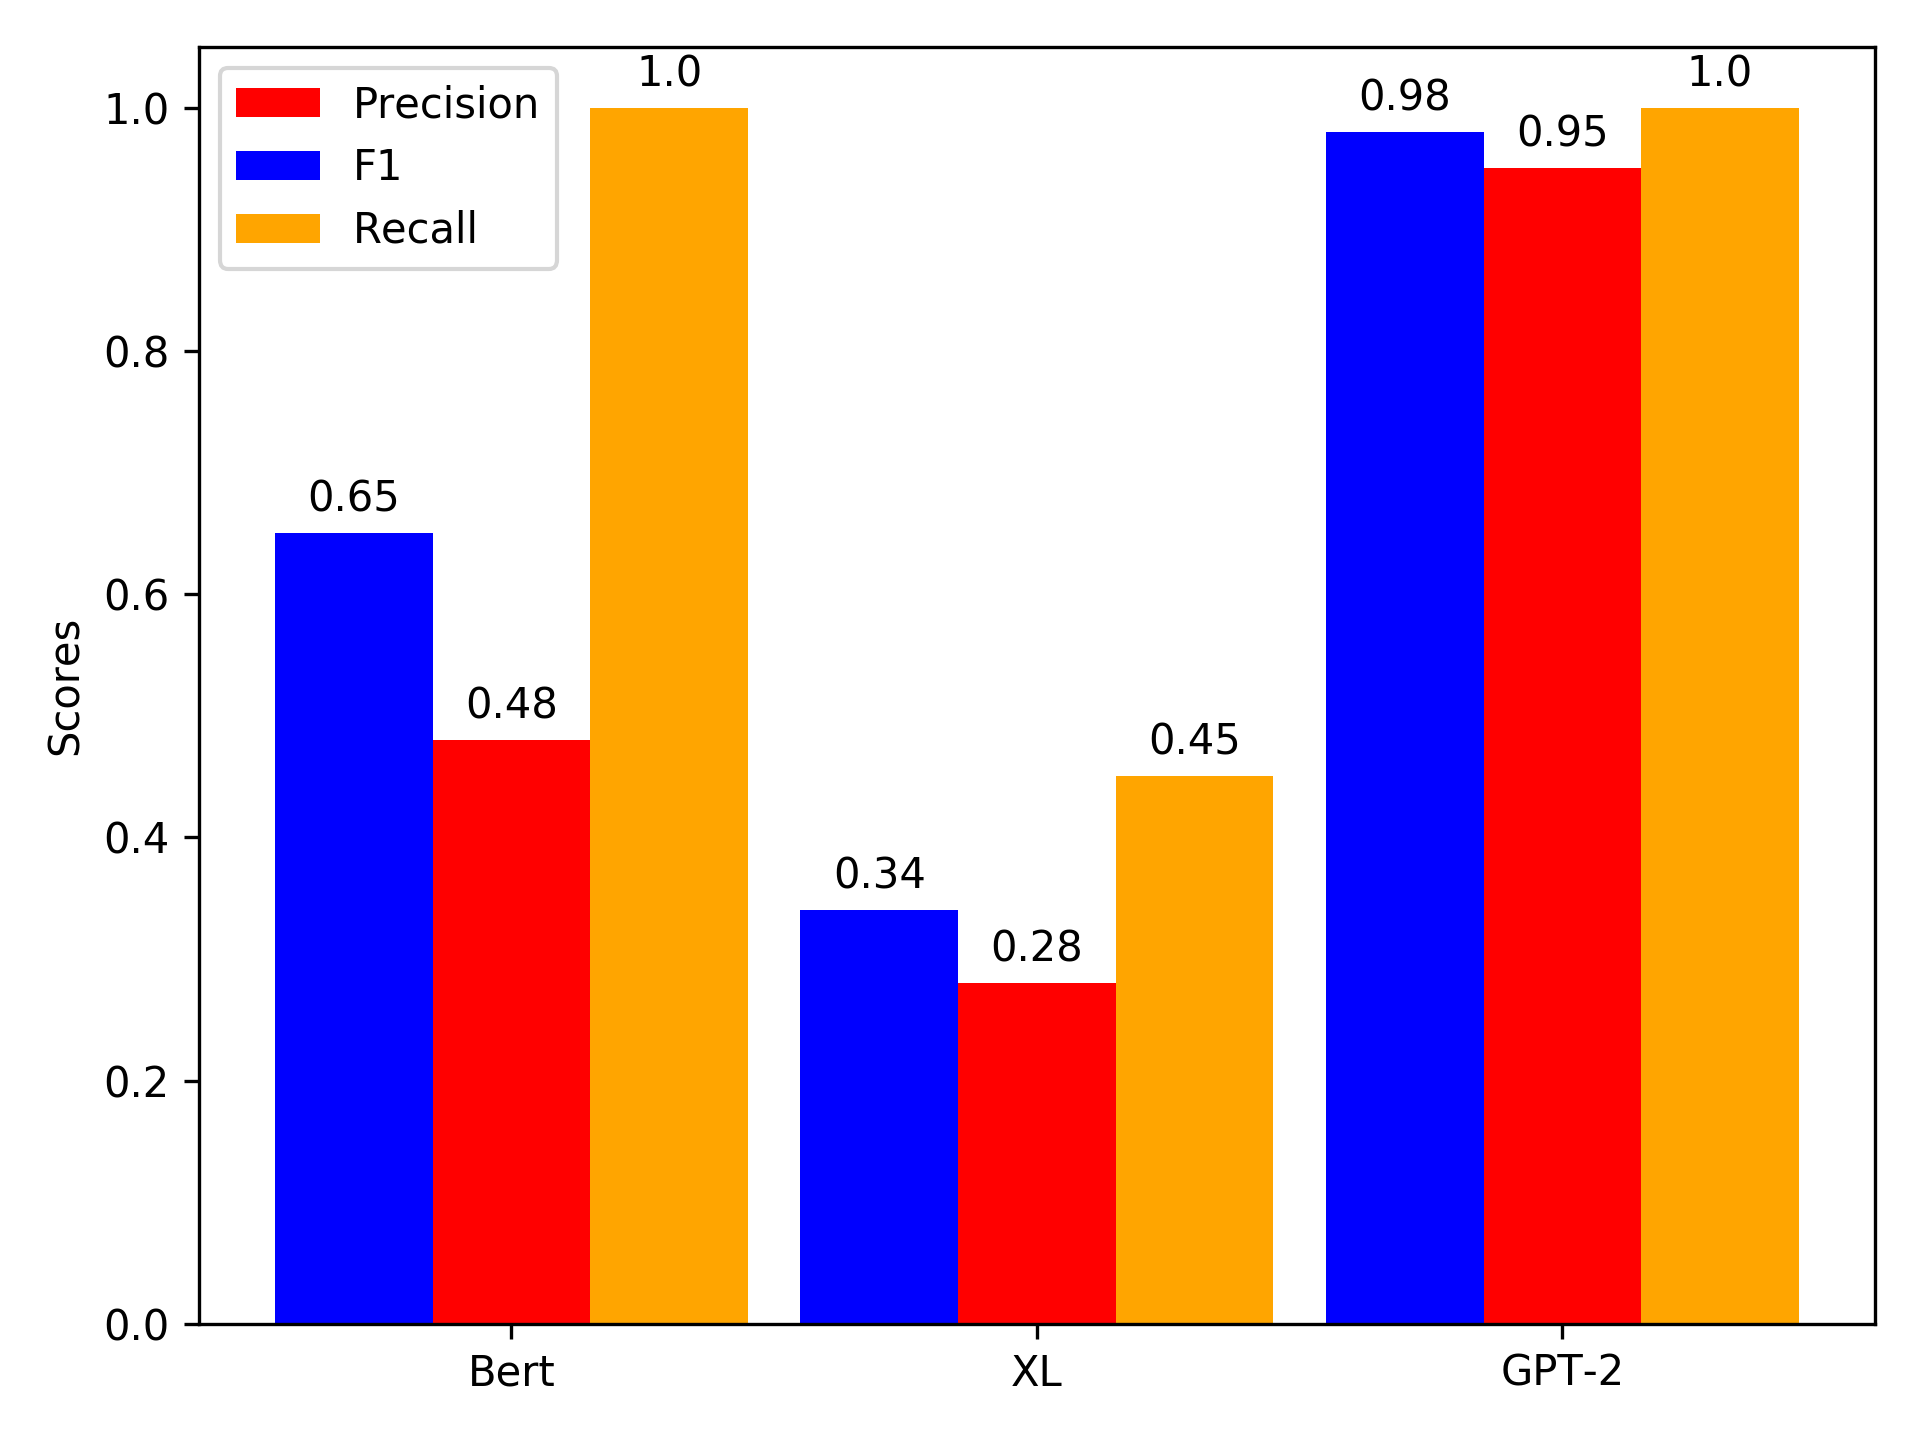
\includegraphics[trim={1cm 0.5cm 0cm 1cm}, width=0.322\textwidth]{results/transfer/transfer_regression_0.1_ratio.png}}
\hspace{\fill}
   \subfloat[15\% alteration\label{fig:results_transfer_regression_0.15}]{%
      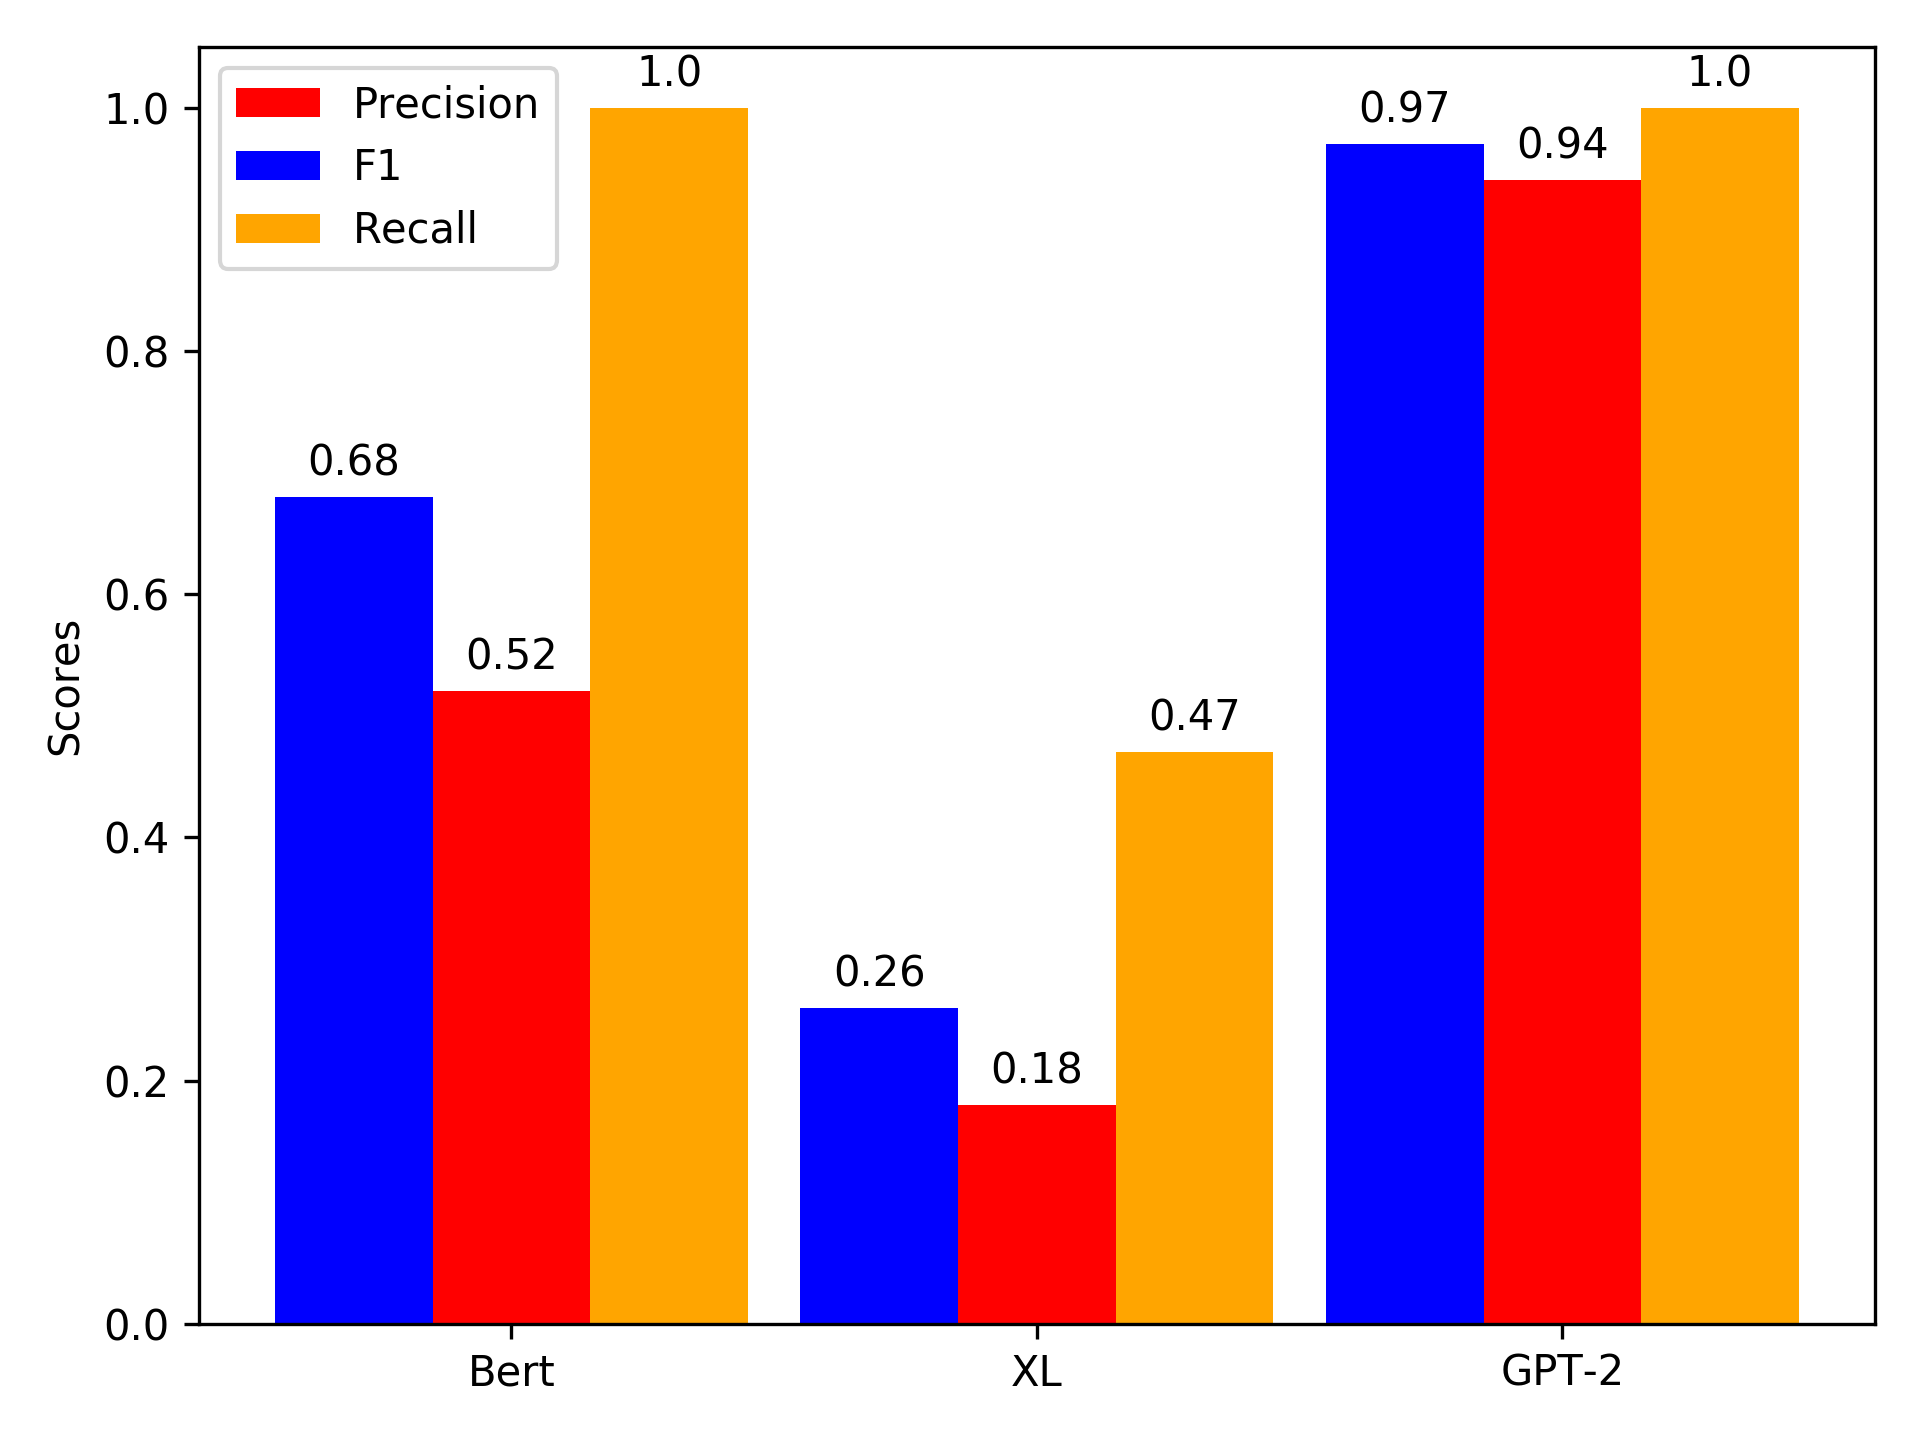
\includegraphics[trim={1cm 0.5cm 0cm 1cm}, width=0.322\textwidth]{results/transfer/transfer_regression_0.15_ratio.png}}\\
\caption{\label{fig:results_transfer_regression}Transfer of knowledge with different ratios of alteration, 5\% semantically different anomalies, using regression.}
\end{figure*}



\begin{comment}
These findings are confirmed by the ROC curve plots which can be seen in figure \ref{fig:results_transfer_regression_roc}, showing nearly perfect results for GPT-2, very good results for Bert and far less satisfying results for XL-Transformers.
\end{comment}

\begin{figure*}[ht!]
\centering
  \captionsetup{justification=centering}
   \subfloat[Bert\label{fig:results_transfer_regression_per_epoch_0.05}]{%
      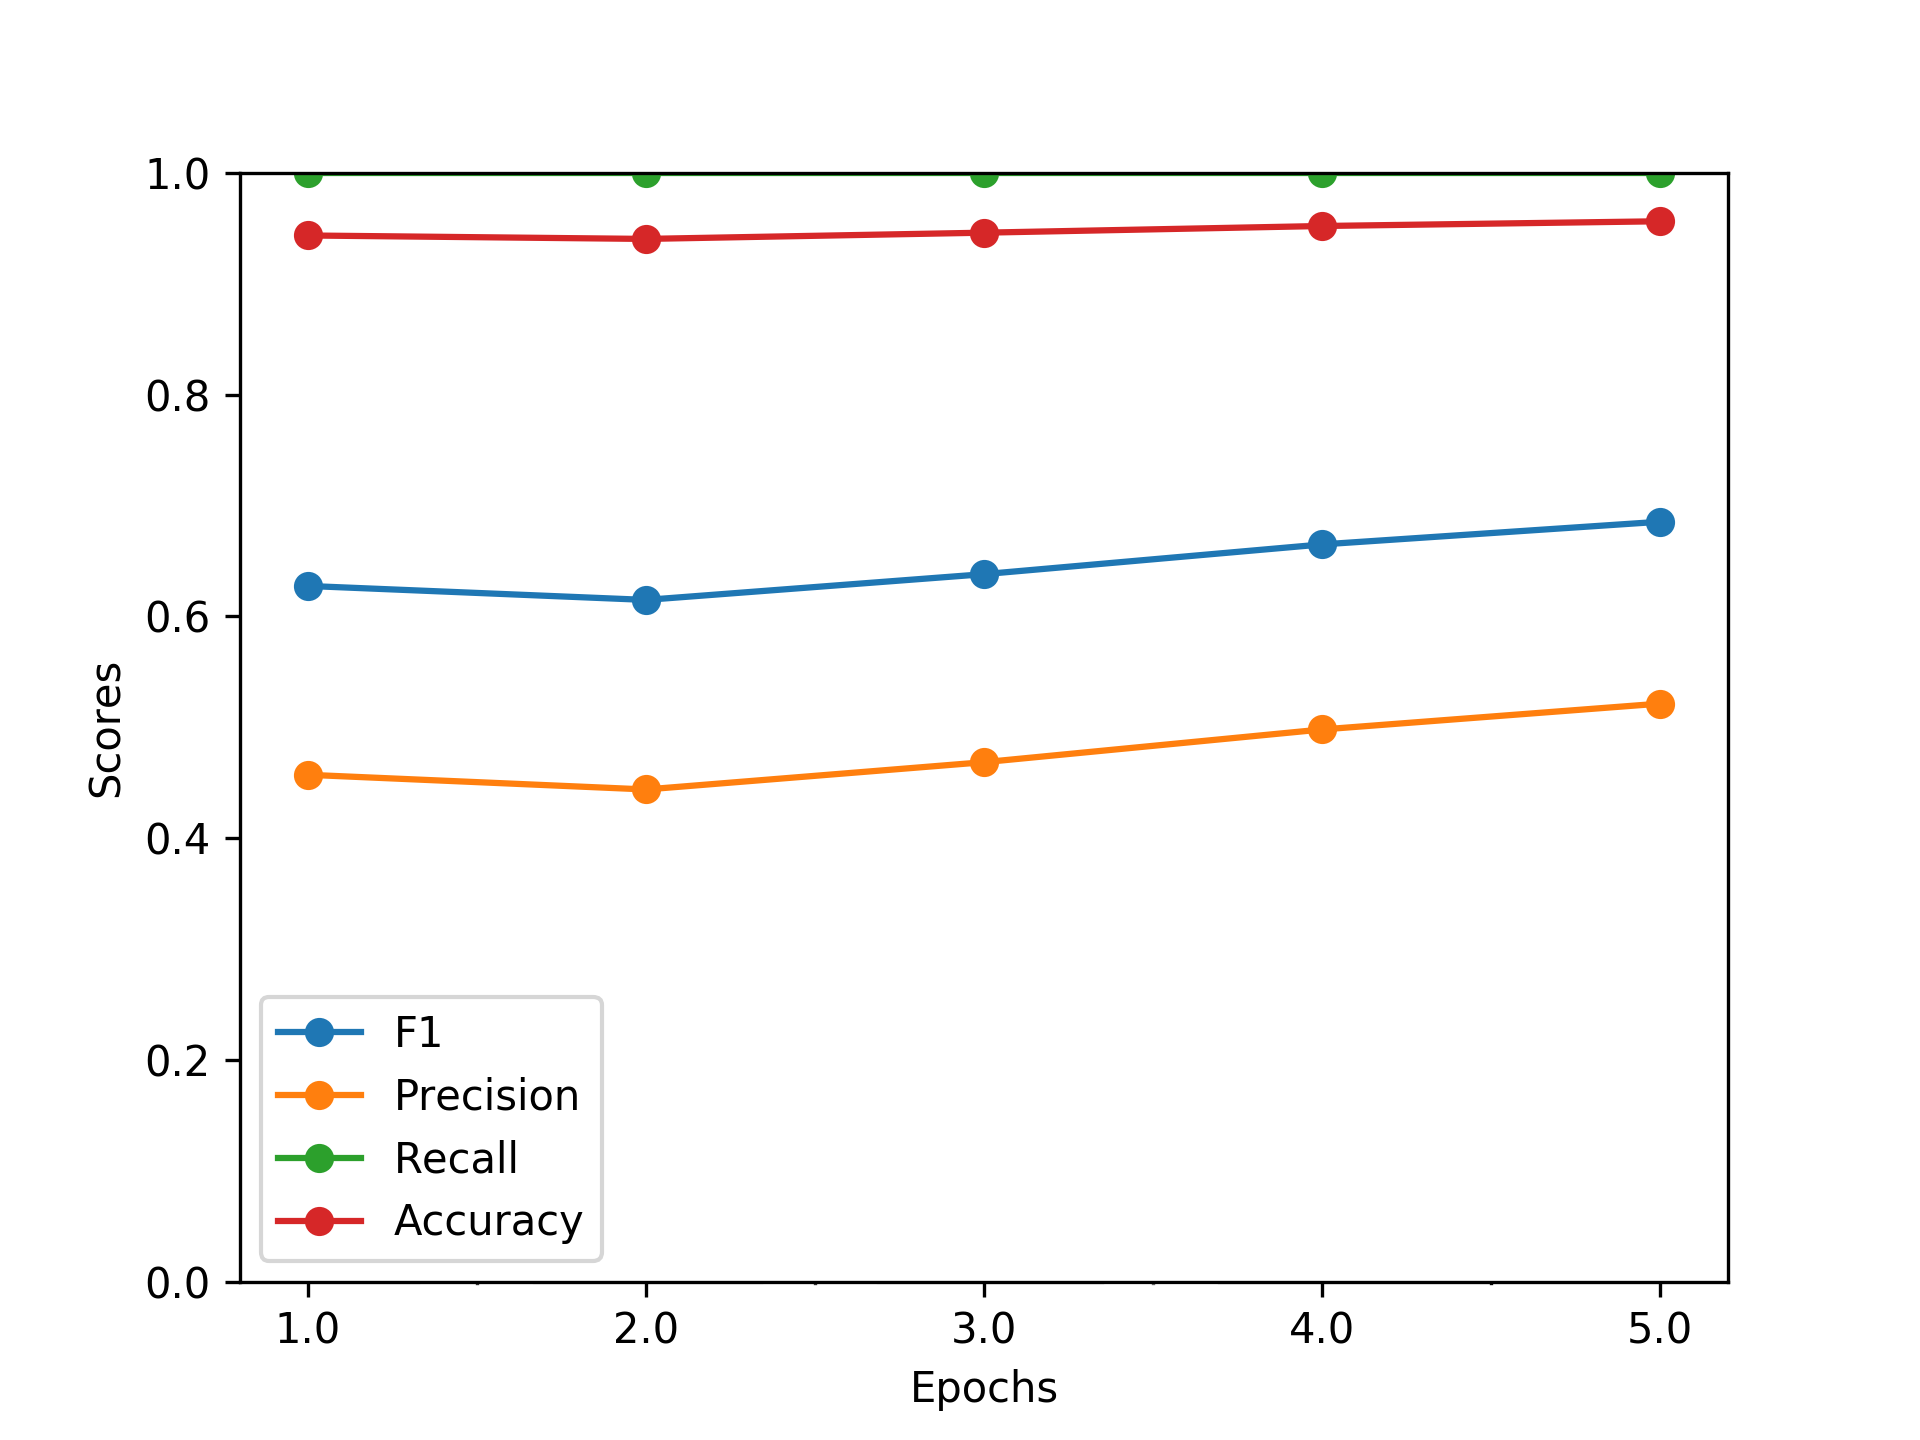
\includegraphics[width=0.322\textwidth]{results/transfer/bert_regression_0.15_transfer_metrics_per_epoch.png}}
\hspace{\fill}
   \subfloat[GPT-2\label{fig:results_transfer_regression_per_epoch_0.10} ]{%
      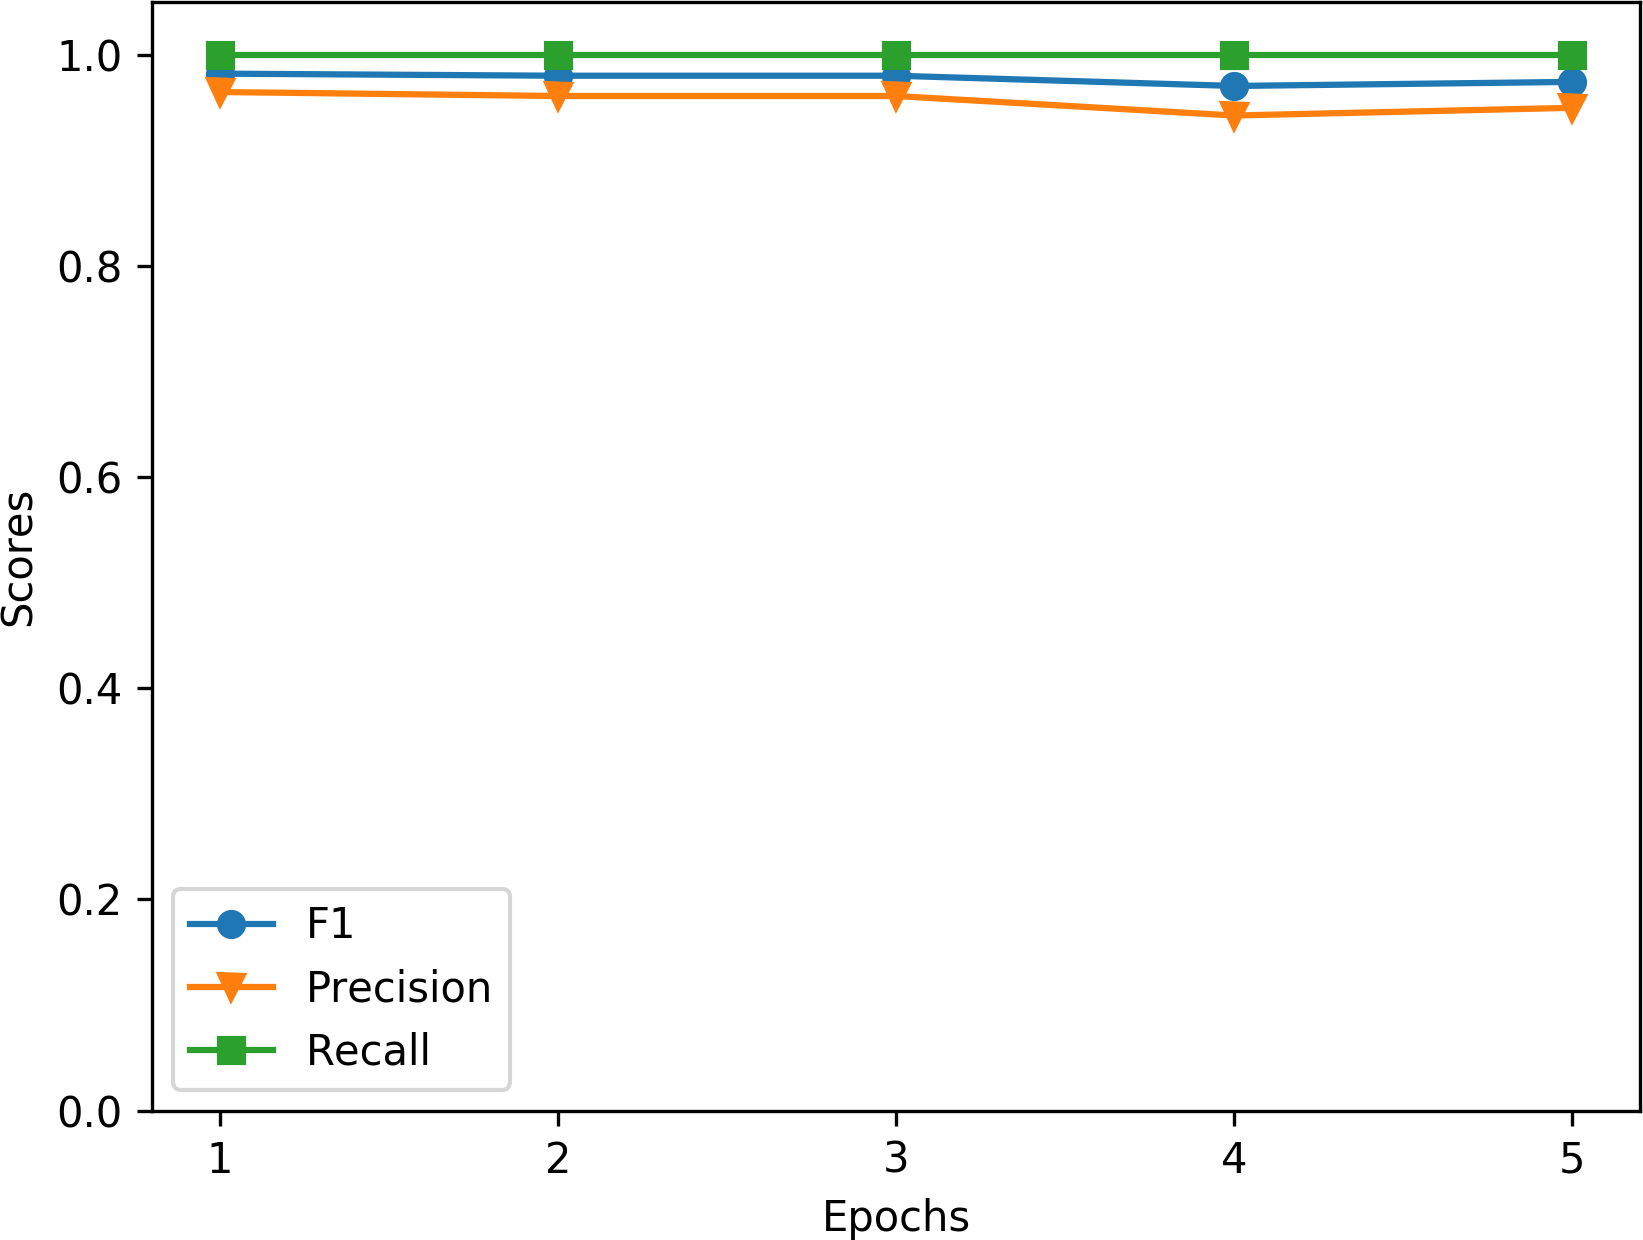
\includegraphics[width=0.322\textwidth]{results/transfer/gpt_regression_0.15_transfer_metrics_per_epoch.png}}
\hspace{\fill}
   \subfloat[XL\label{fig:results_transfer_regression_per_epoch_0.15}]{%
      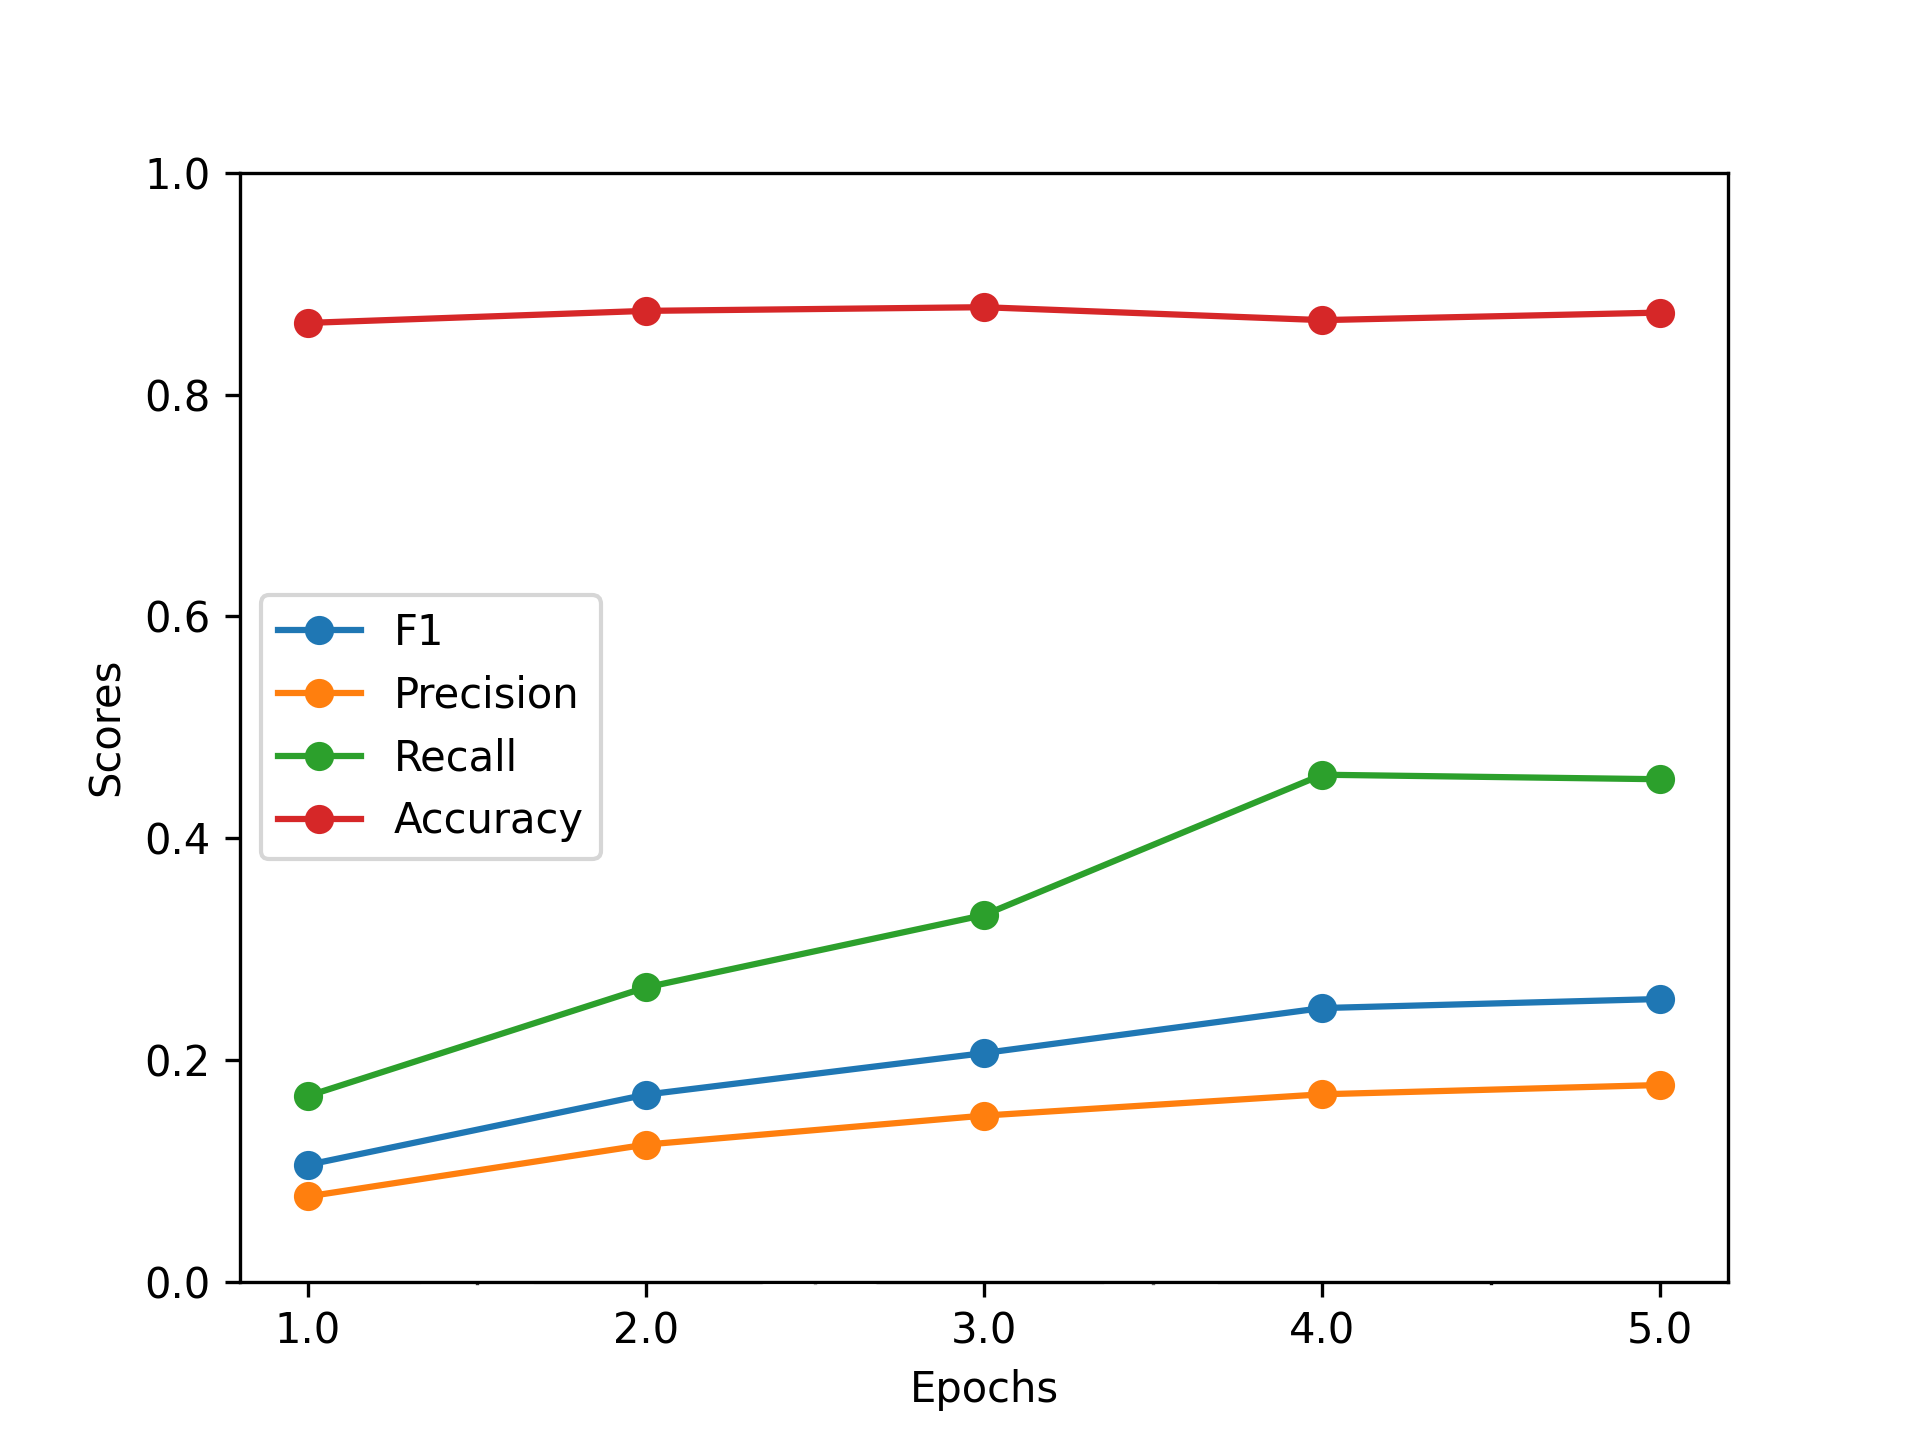
\includegraphics[width=0.322\textwidth]{results/transfer/xl_regression_0.15_transfer_metrics_per_epoch.png}}\\
\caption{\label{fig:results_transfer_regression_per_epoch}Improvement of metrics for transfer of knowledge per additional learning epoch, with 15\% alterations and injection of semantically different anomalies, using regression.}
\end{figure*}

\begin{comment}
\begin{figure*}[ht!]
\centering
  \captionsetup{justification=centering}
   \subfloat[Bert\label{fig:roc_curve_bert_transfer_regression}]{%
      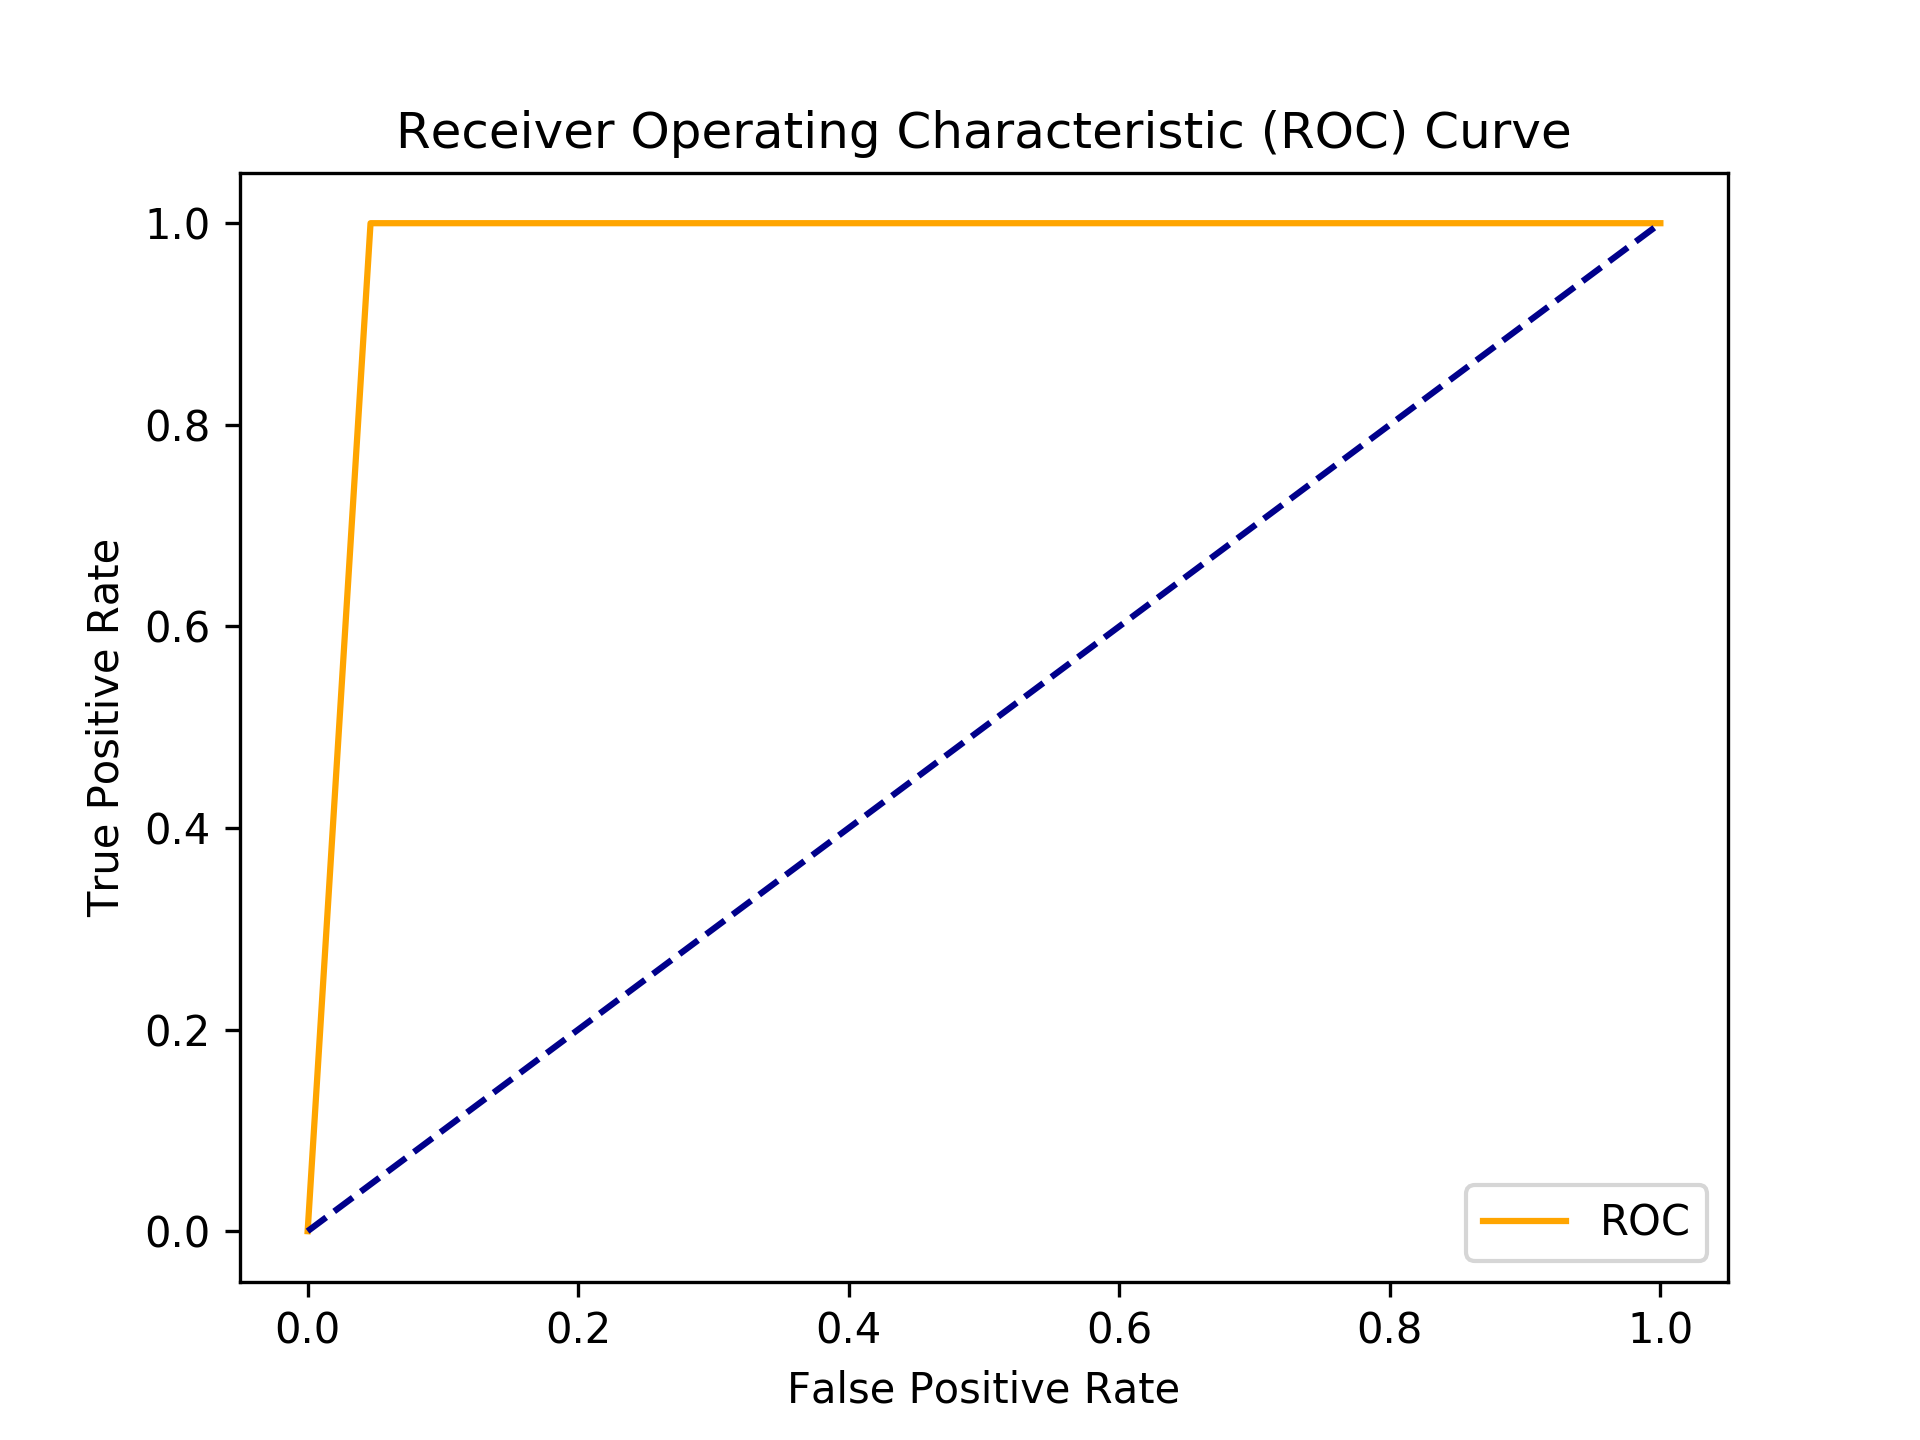
\includegraphics[trim={1cm 0.5cm 0cm 1cm}, width=0.322\textwidth]{results/transfer/roc_curve_transfer_regression_bert_0.15.png}}
\hspace{\fill}
   \subfloat[GPT-2\label{fig:roc_curve_gpt_transfer_regression} ]{%
      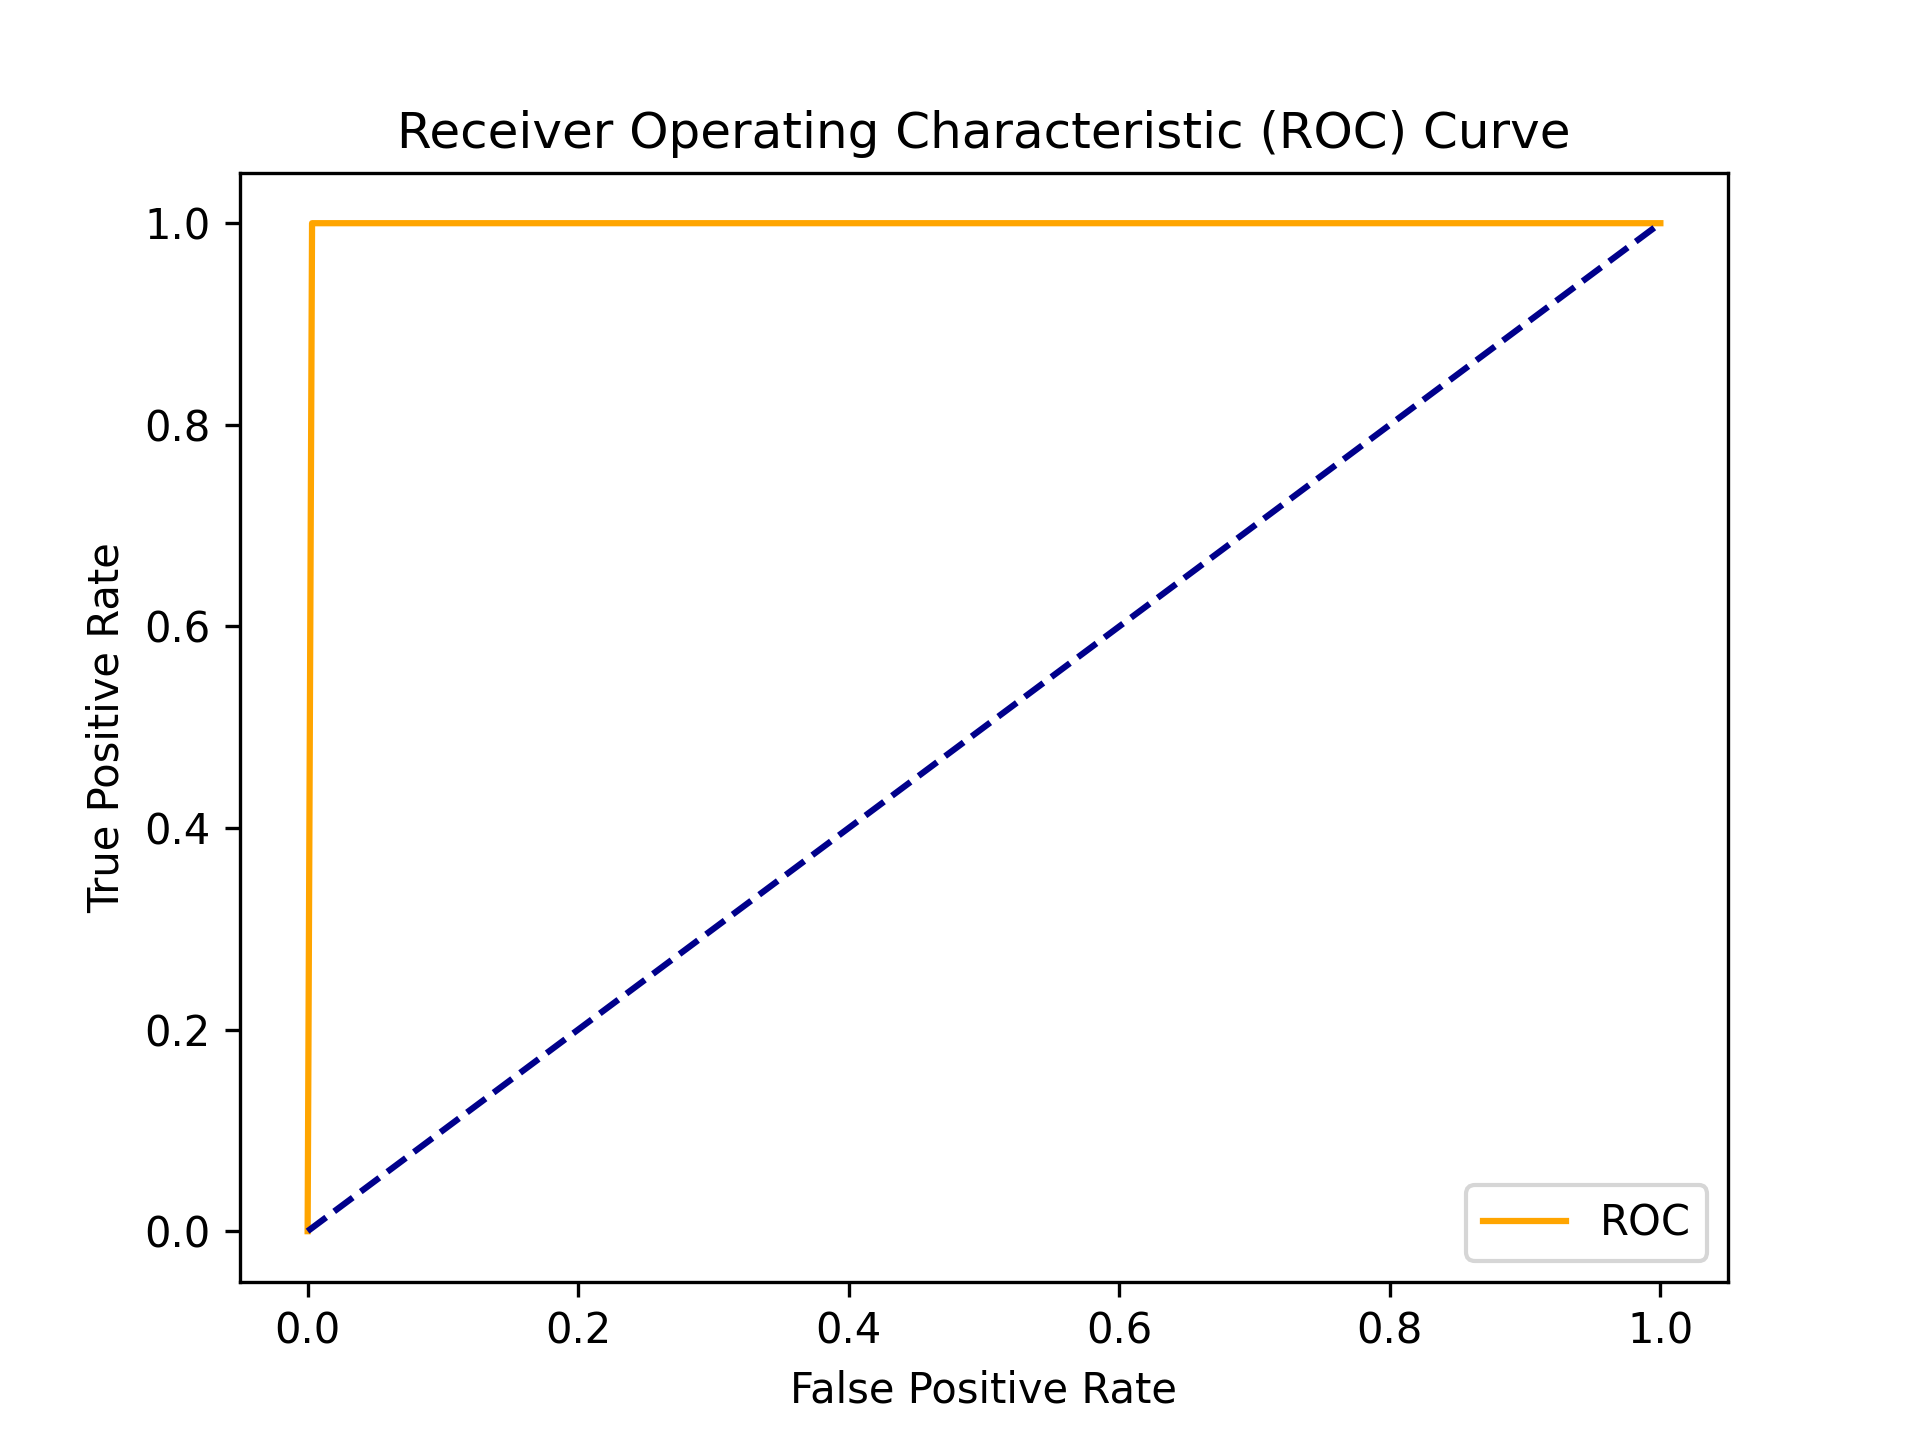
\includegraphics[trim={1cm 0.5cm 0cm 1cm}, width=0.322\textwidth]{results/transfer/roc_curve_transfer_regression_gpt_0.15.png}}
\hspace{\fill}
   \subfloat[XL\label{fig:roc_curve_xl_transfer_regression}]{%
      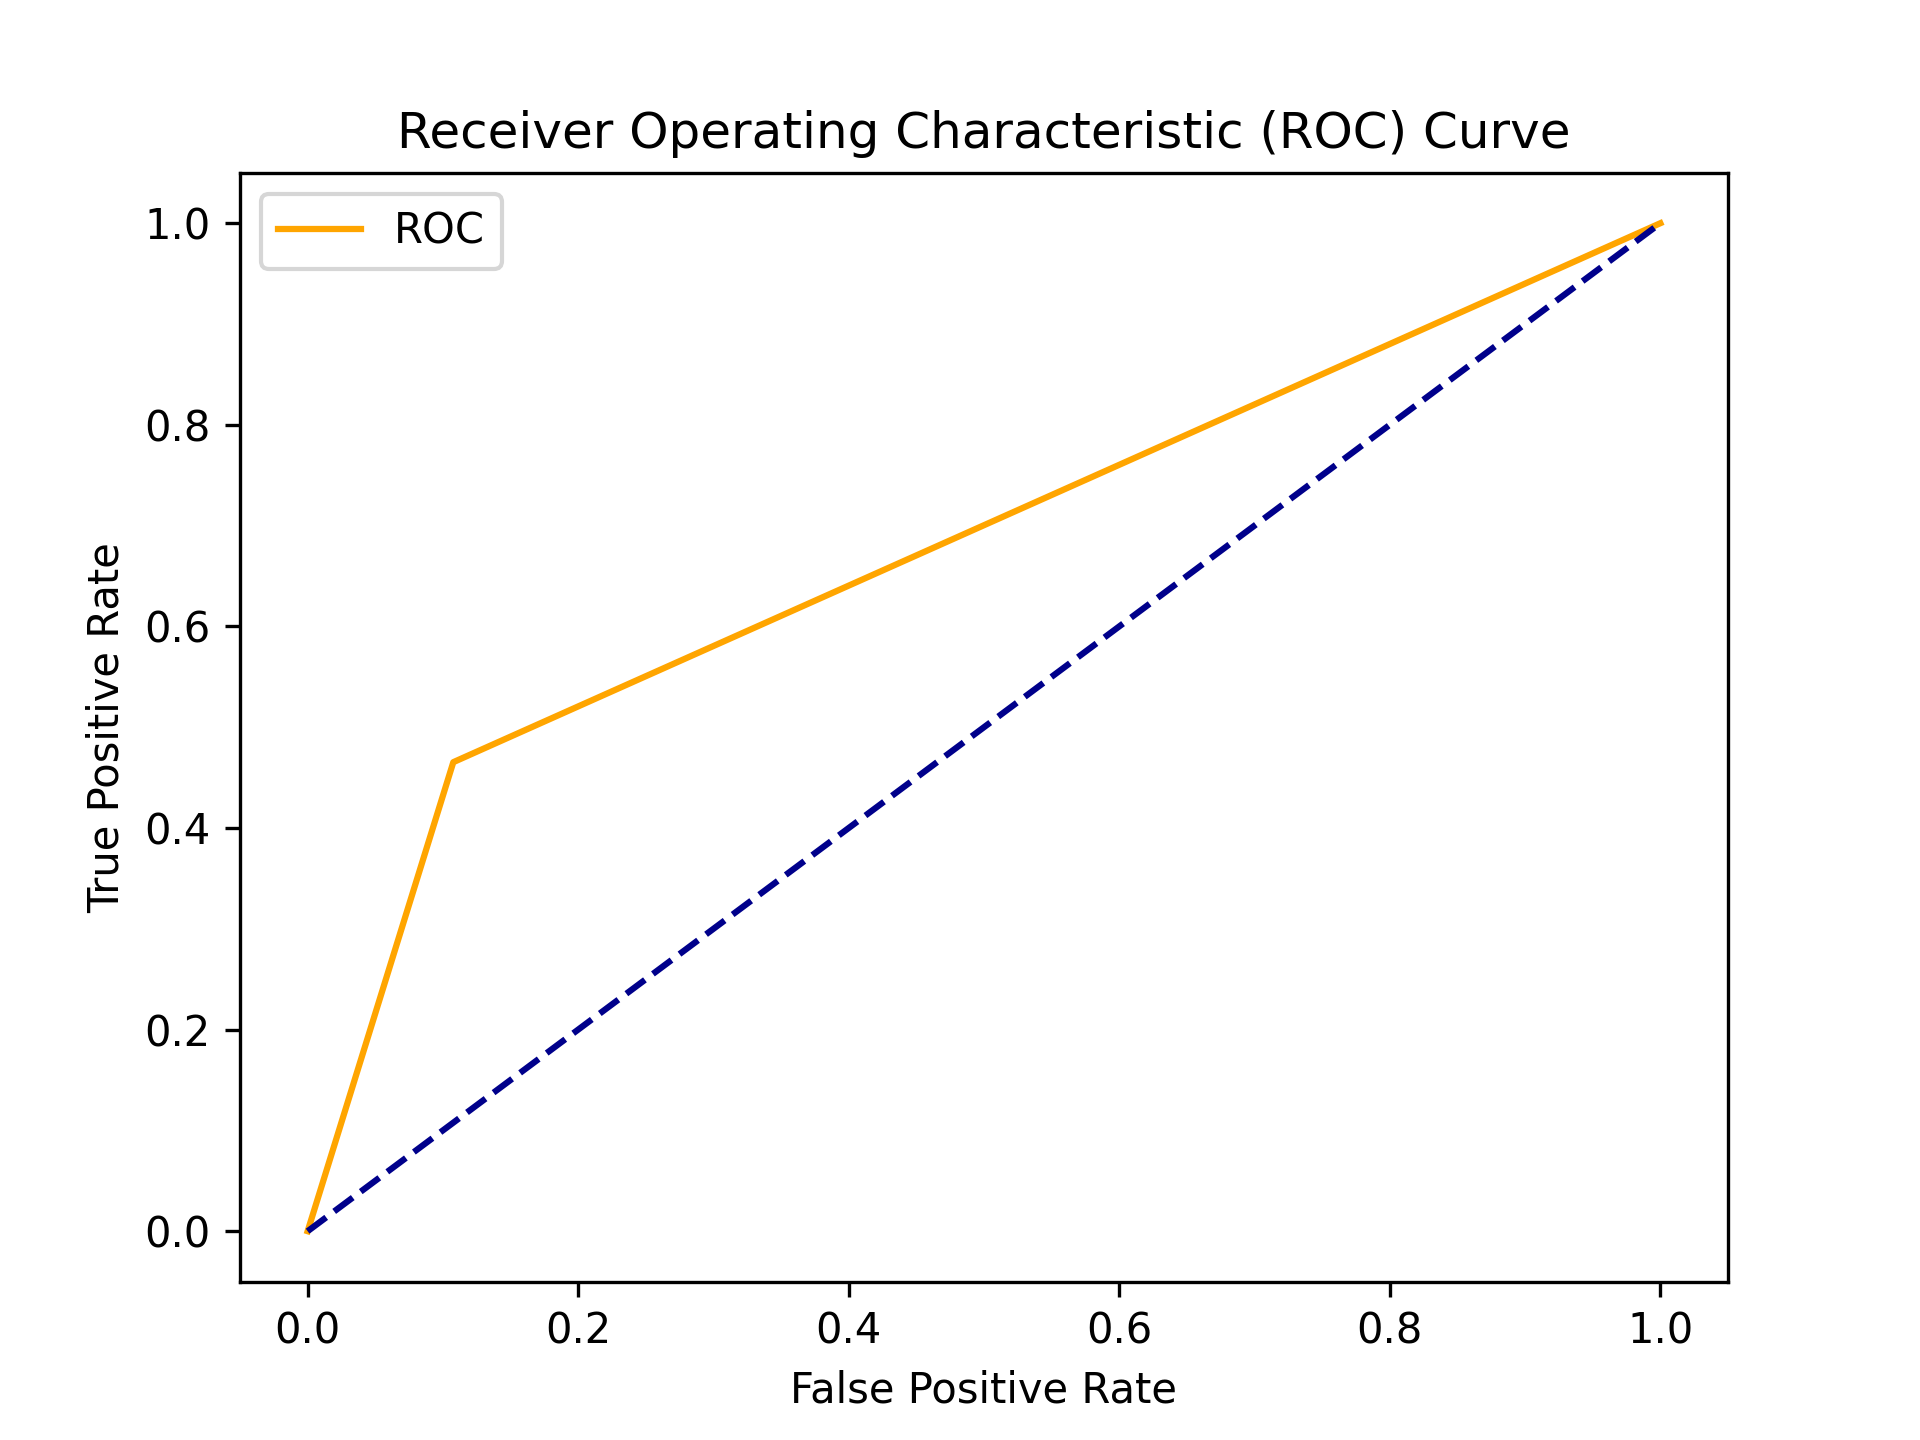
\includegraphics[trim={1cm 0.5cm 0cm 1cm}, width=0.322\textwidth]{results/transfer/roc_curve_transfer_regression_xl_0.15.png}}\\
\caption{\label{fig:results_transfer_regression_roc}ROC-Curve for transfer of knowledge using regression with 15\% alterations.}
\end{figure*}
\end{comment}

\begin{figure}[H]
  \centering
  \captionsetup{justification=centering}
  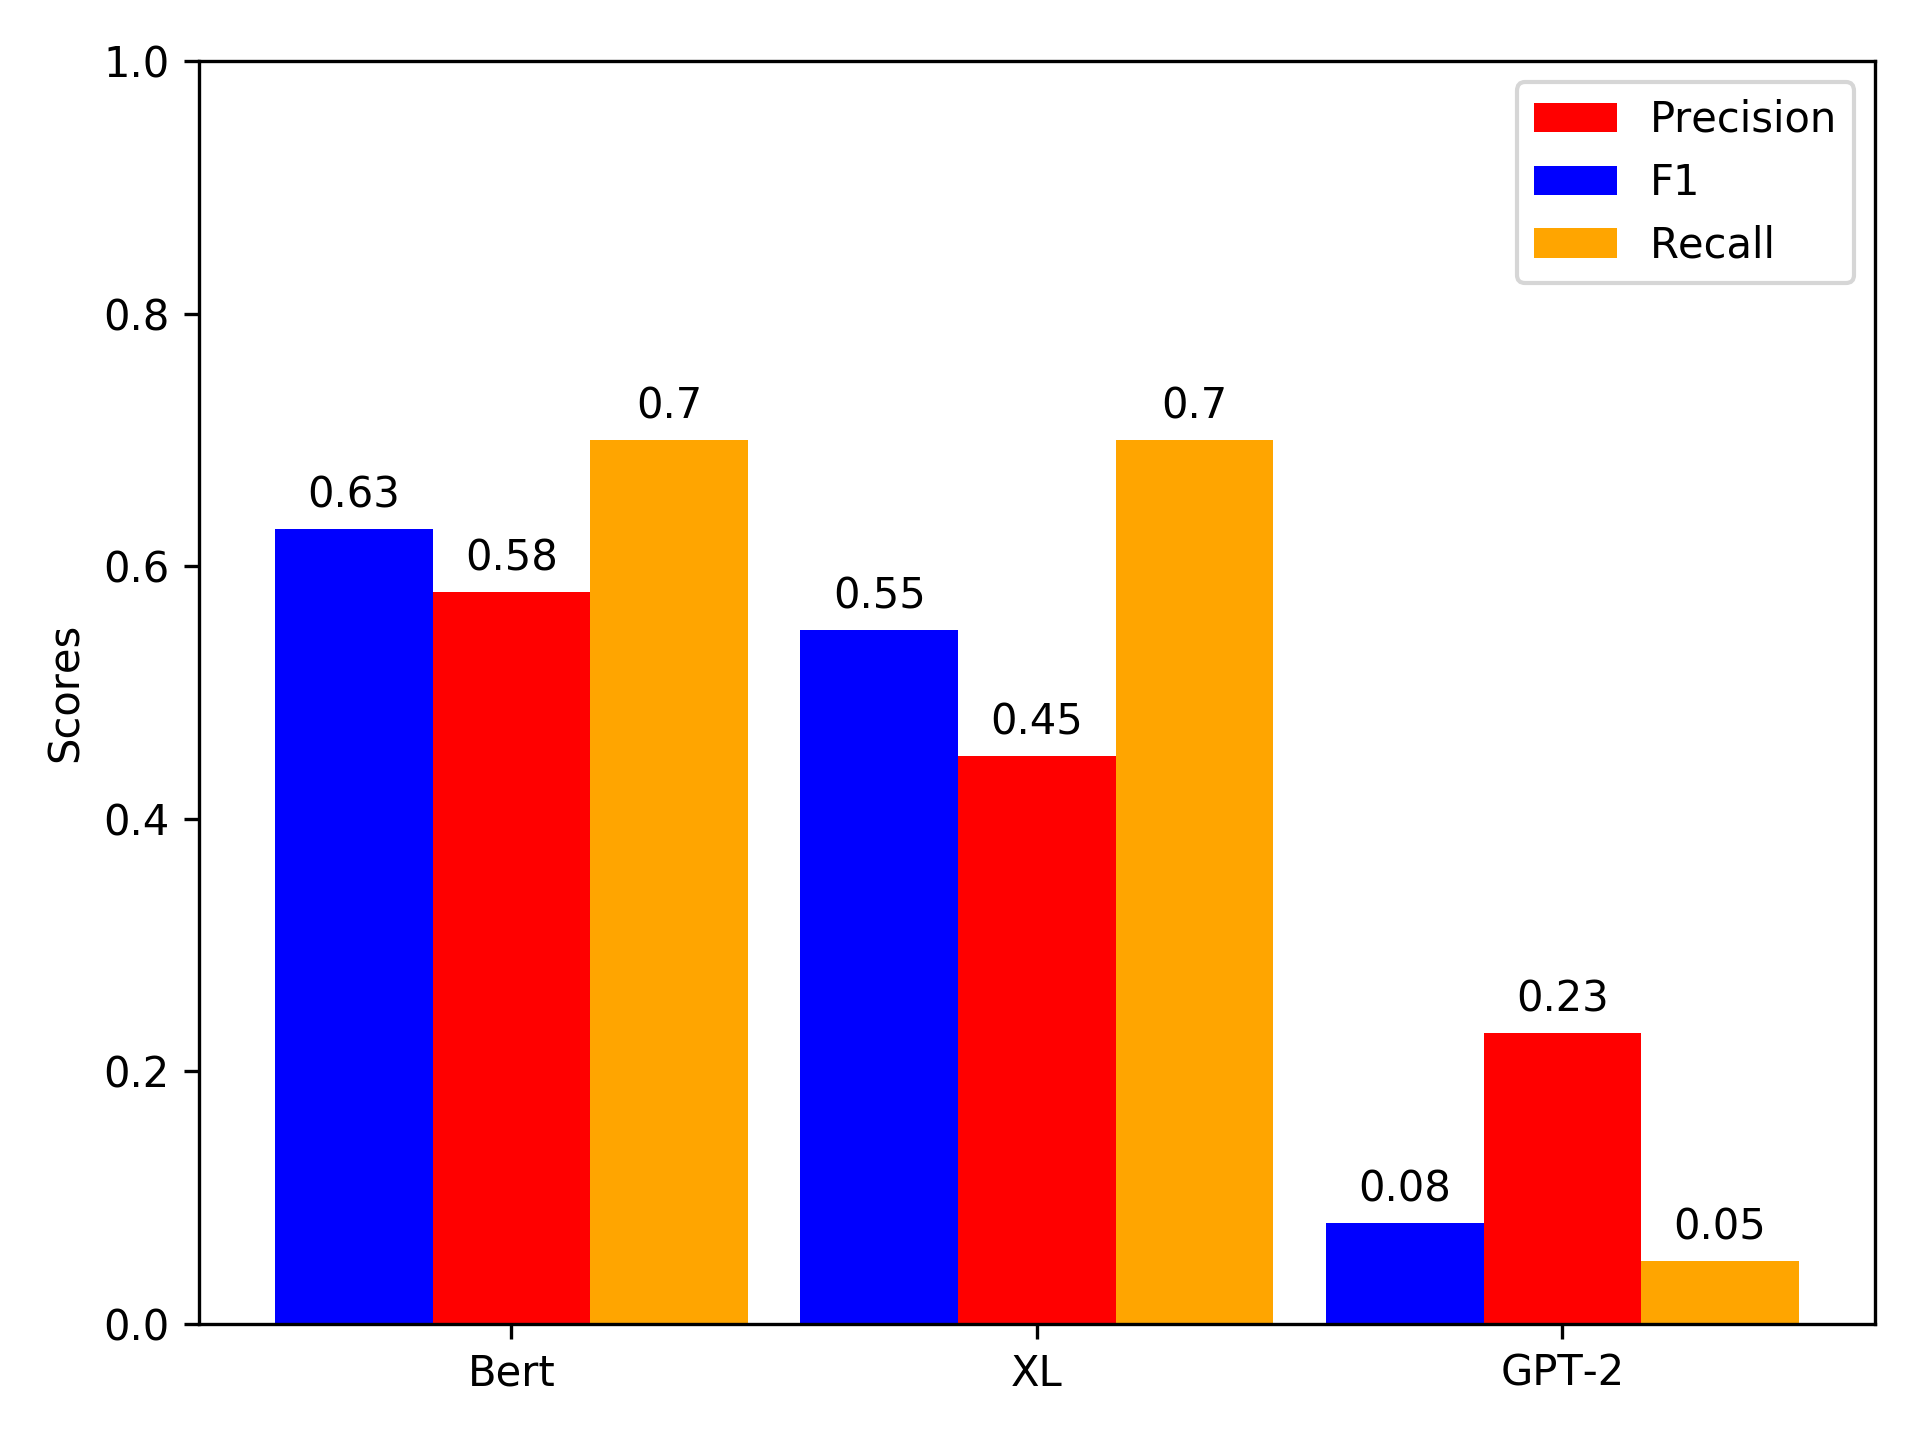
\includegraphics[width=8cm]{results/transfer_regression_replace_half.png}\\
  \caption{Transfer of knowledge. 15\% alteration, injection of semantically similar anomalies, using regression.}
  \label{fig:replace_words_regression_transfer}
\end{figure}

%%%% TRANSFER LEARNING CLASSIFICATION
\subsection{Transfer of Knowledge Using Classification \label{sec:results-classification-transfer}}

For transfer of knowledge using the classification-based approach, the same experiments as described in \ref{sec:results-regression-transfer} were conducted. Figure \ref{fig:results_transfer_classification} shows the results of the transfer of knowledge experiment with injection of semantically different anomalies. Interesting observations include the stable results achieved using Bert which are little sensitive to increasing alteration ratios. Bert achieves a F1-score of 0.82 for 5\% alterations, 0.77 for 10\% alterations and 0.81 for 15\% alterations, and precision of 0.7 for 5\% alterations, 0.63 for 10\% alterations and 0.68 for 15\% alterations. For XL-Transformers, the F1-score is 0.46 for 5\% alterations, 0.61 for 10\% alterations and 0.38 for 15\% alterations, while precision goes from 0.3 for 5\% alterations to 0.44 for 10\% alterations to 0.23 for 15\% alterations. GPT-2 shows overall less useful results than for the regression approach and the injection of semantically different anomalies, with a F1-score of 0.23 for 5\% alterations, 0.18 for 10\% alterations and 0.17 for 15\% alterations, precision of 0.13 for 5\% alterations, 0.1 for 10\% alterations and 0.09 for 15\% alterations, and a recall of 1.0 for all injection ratios.

The results show that Bert has clear advantages over GPT-2 and XL-Transformers for the classification-based approach. It is noticeable, that all language models achieve a recall value of 1.0. This is due to the high cosine distance of the injected semantically different anomaly log event.

Figure \ref{fig:results_transfer_multiclass_per_epoch} depicts the development of the metrics of detecting semantically different anomalies for every additional epoch of training on dataset $B$. After every epoch of training on the train dataset $B$, the labelled test dataset $B$ is fed into the model, and metrics are collected. Bert improves the most per epoch, with an initial F1-score of  0.3 for one epoch of training to 0.81 after 5 epochs, and precision of 0.18 after one epoch to 0.68 after 5 epochs. GPT-2 shows no significant changes, while XL-Transformers improves its F1-score from 0.24 after one epoch to 0.38 after 5 epochs and precision from 0.17 after one epoch to 0.23 after 5 epochs. All language models start with a recall value of 1.0 after one epoch which stays the same after 5 epochs.

%These findings are confirmed by the ROC curve plots which can be seen in figure \ref{fig:results_transfer_multiclass_roc}, showing very good results for Bert, acceptable results for Xl-Transformers and far less satisfying results for GPT-2.


The results for injecting 5\% semantically similar anomalies for transfer of knowledge with 15\% alterations using classification can be seen in figure \ref{fig:replace_words_classification_transfer}. In comparison to the usage of the regression-based approach for transfer of knowledge and injection of semantically similar anomalies as explained in \ref{sec:results-regression-transfer} and depicted in \ref{fig:replace_words_regression_transfer}, all three language models achieve better results, especially GPT-2. All three language models also achieve a recall value of 1.0. Bert achieves a F1-score of 0.75 and a precision of 0.61, XL-Transformers achieves a F1-score of 0.69 and a precision of 0.53, GPT-2 achieves a F1-score of 0.43 and precision of 0.27. Bert is obviously the most fit for the task of anomaly detection using the classification-based approach, for injection of semantically different and semantically similar anomalies.

%\begin{figure}[h]
%  \centering
%  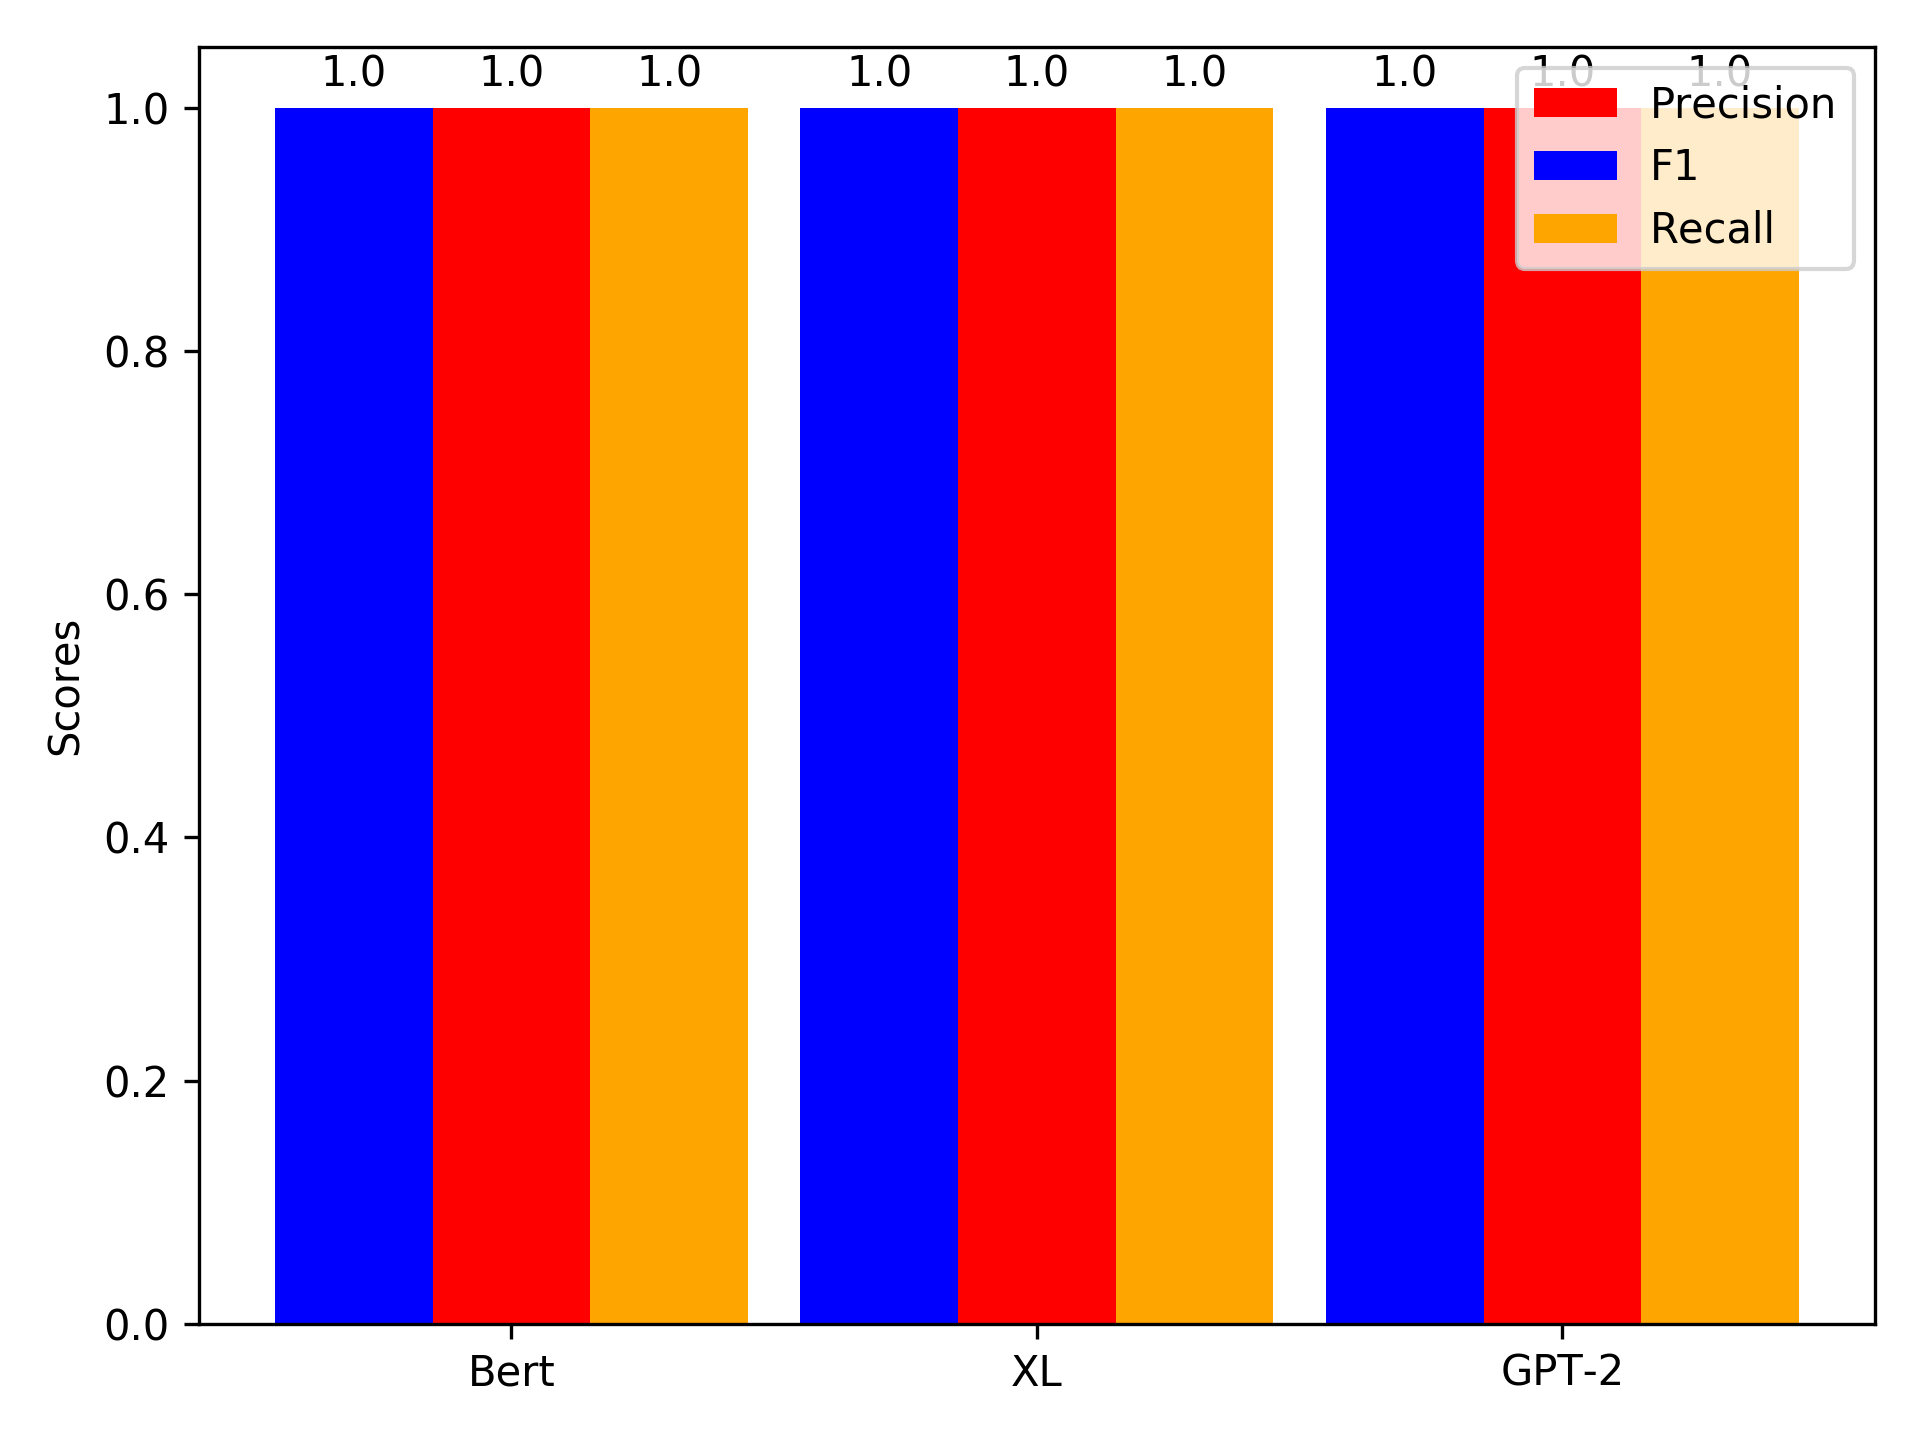
\includegraphics[width=6cm,height=4.5cm]{results/transfer/transfer_classification_reverse.png}\\
%  \caption{Scores for detecting reversed order of log events for transfer learning, using classification.}
%  \label{fig:classification_transfer_reverse}
  
%\end{figure}
\begin{figure*}[ht!]
\centering
  \captionsetup{justification=centering}
   \subfloat[5\% alteration\label{fig:results_transfer_classification_0.05}]{%
      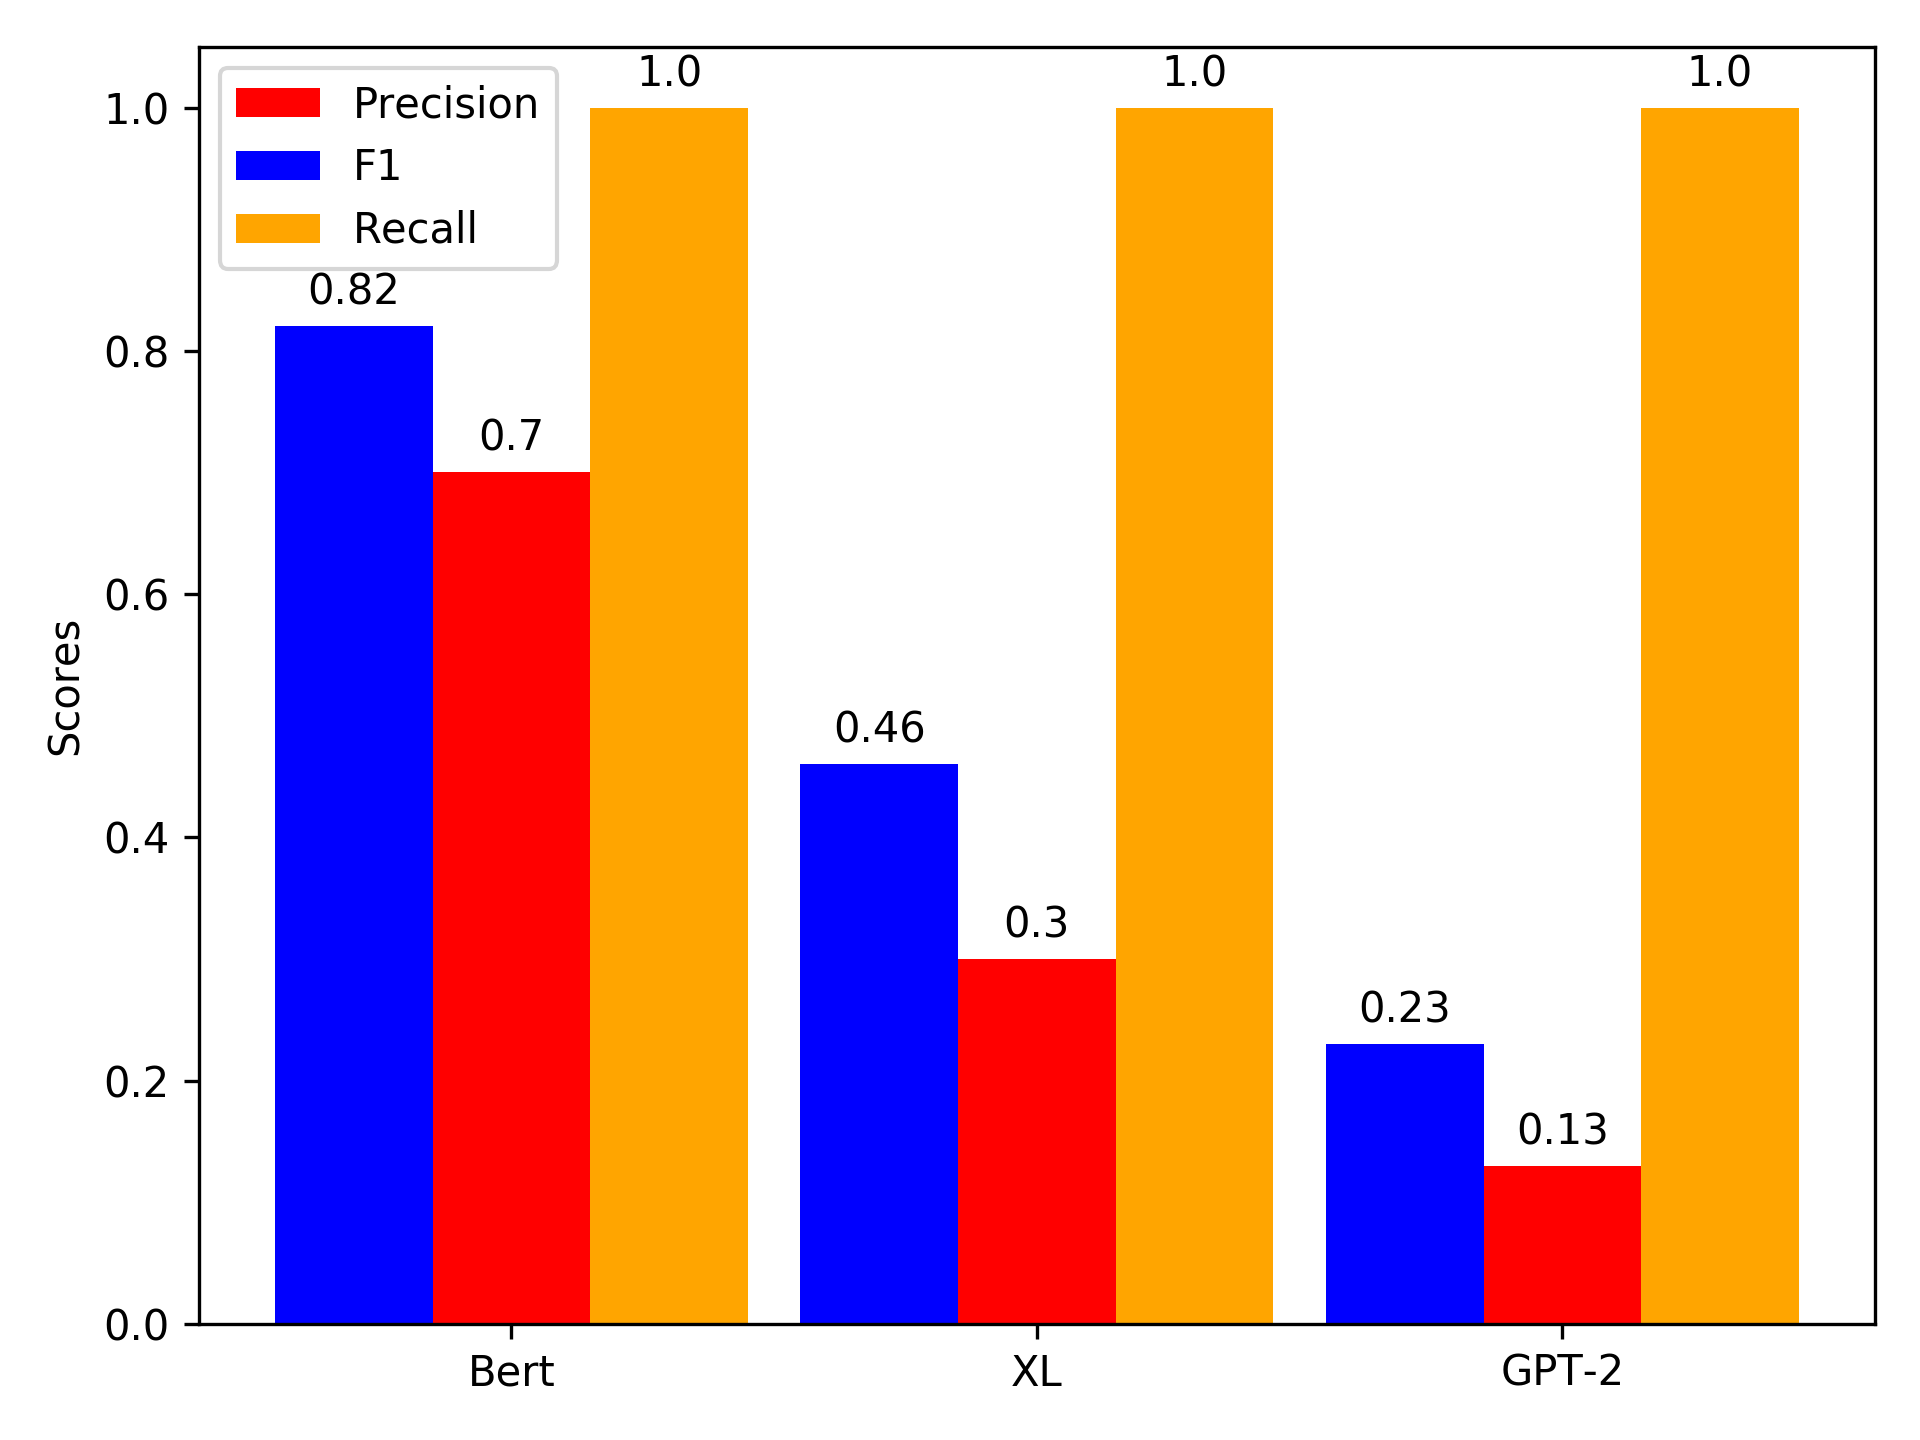
\includegraphics[trim={1cm 0.5cm 0cm 1cm}, width=0.322\textwidth]{results/transfer/transfer_multiclass_0.05_ratio.png}}
\hspace{\fill}
   \subfloat[10\% alteration\label{fig:results_transfer_classification_0.10} ]{%
      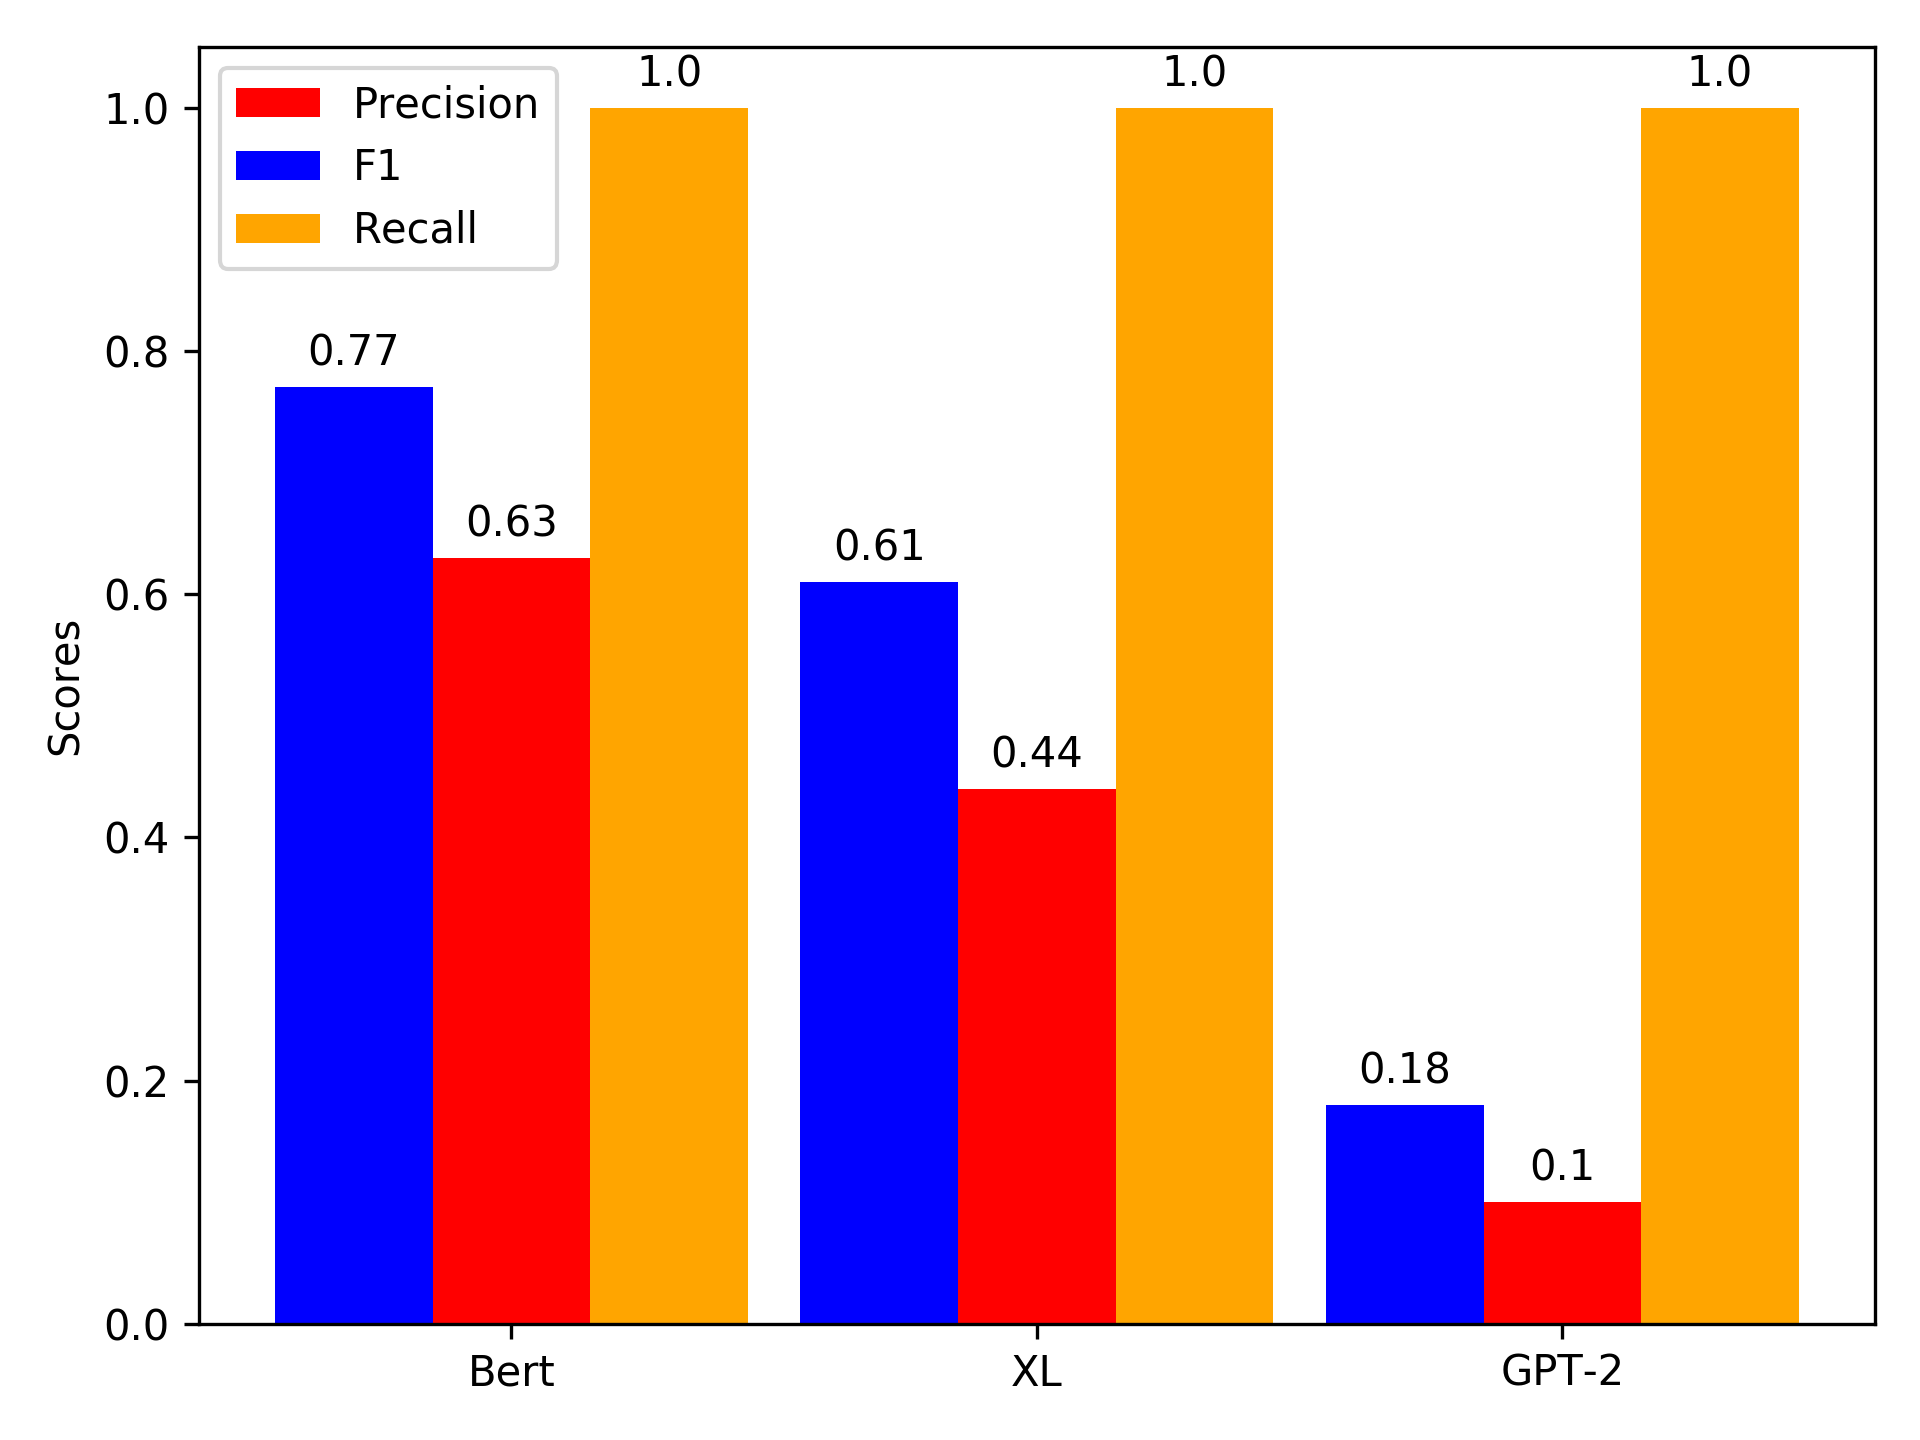
\includegraphics[trim={1cm 0.5cm 0cm 1cm}, width=0.322\textwidth]{results/transfer/transfer_multiclass_0.1_ratio.png}}
\hspace{\fill}
   \subfloat[15\% alteration\label{fig:results_transfer_classification_0.15}]{%
      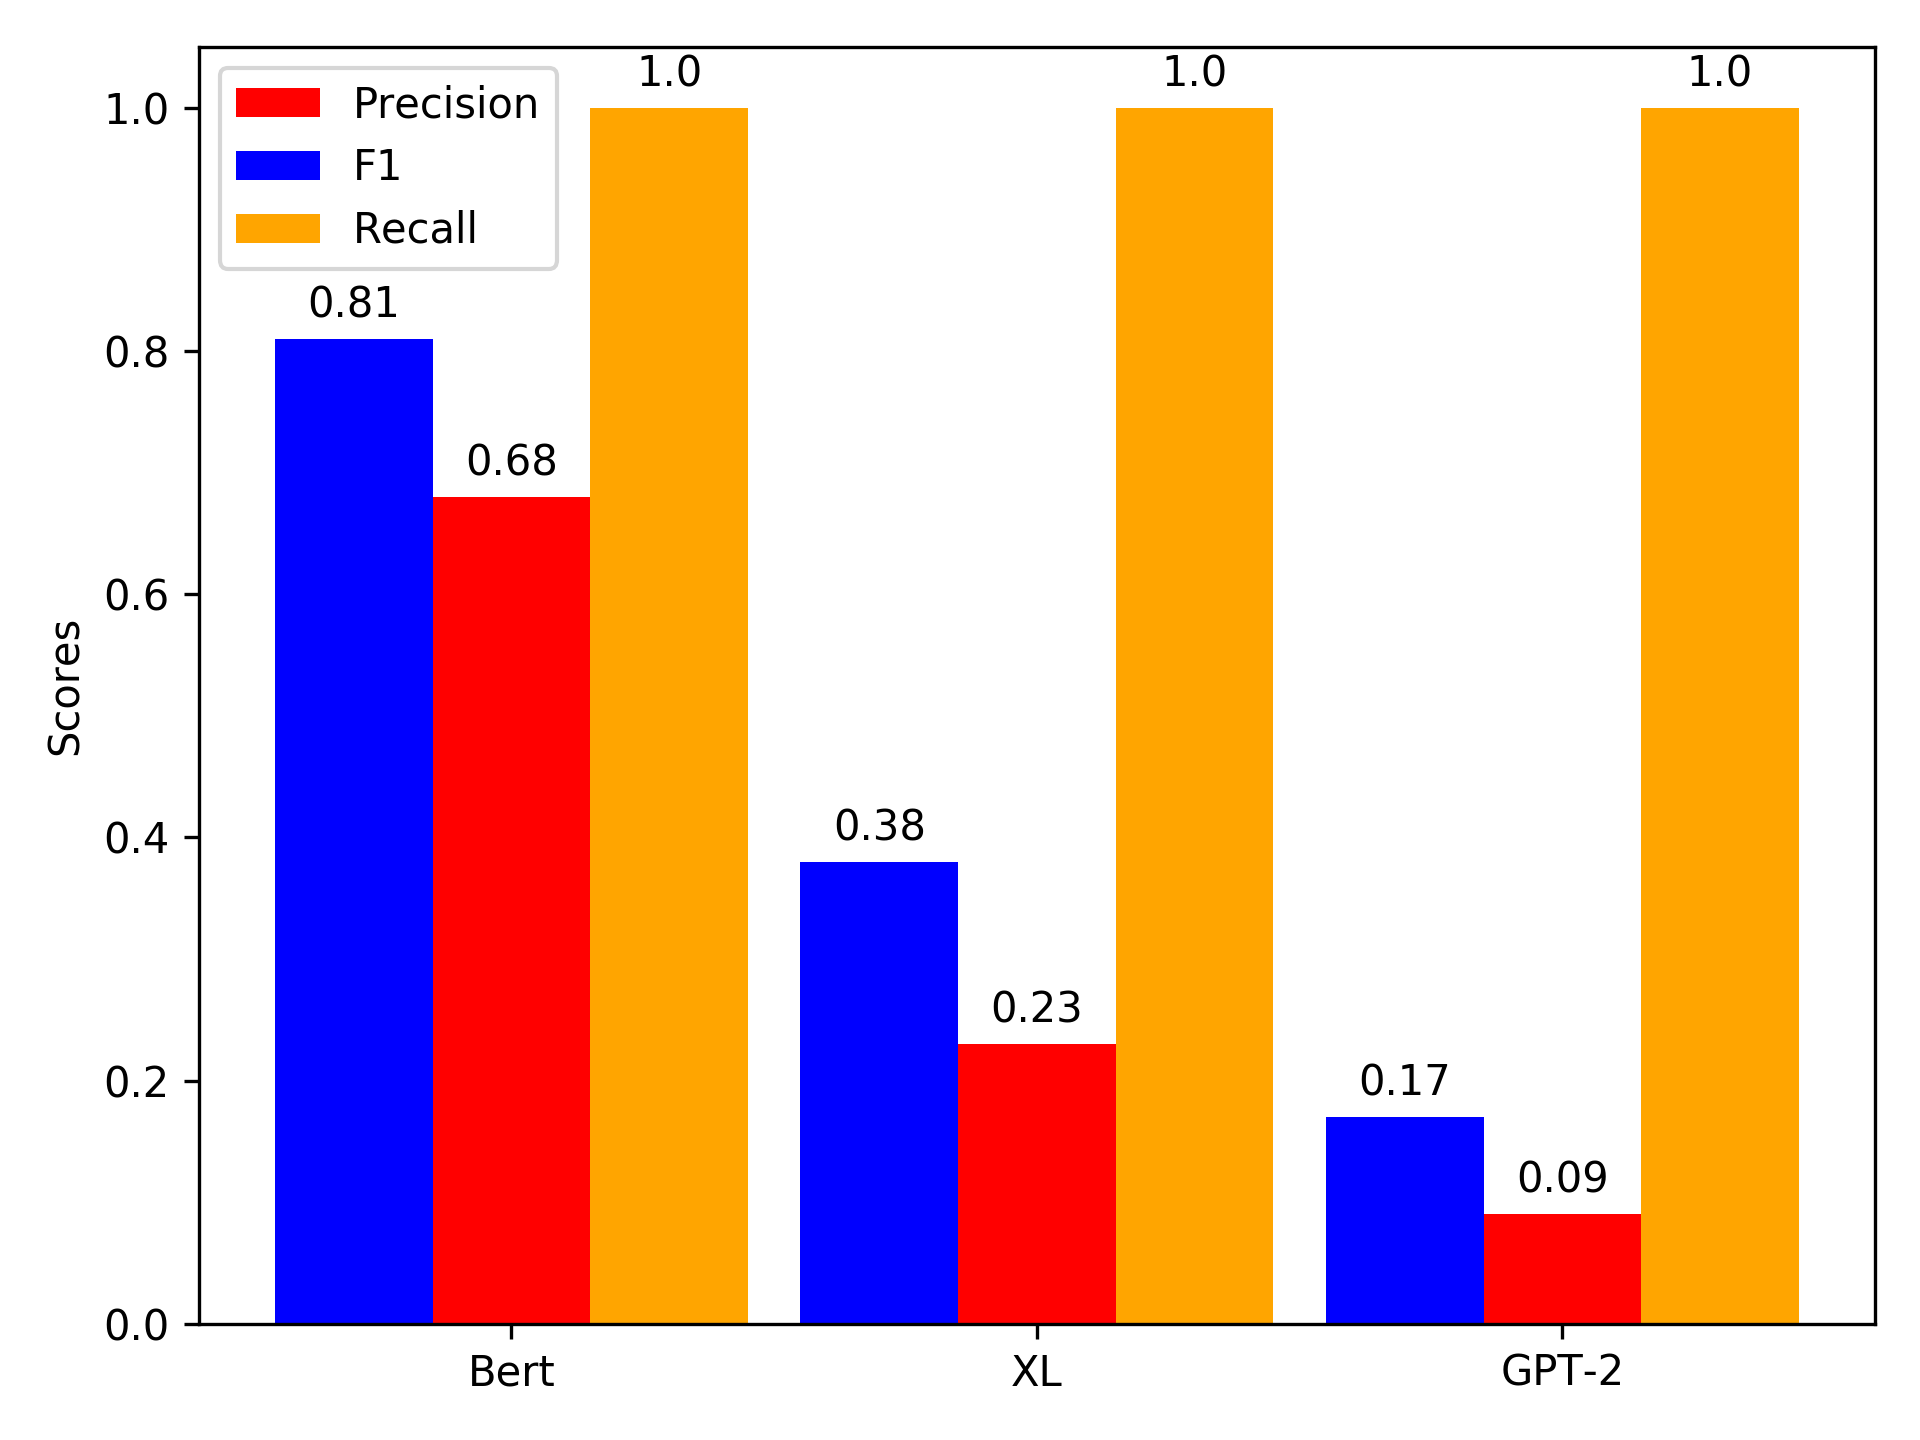
\includegraphics[trim={1cm 0.5cm 0cm 1cm}, width=0.322\textwidth]{results/transfer/transfer_multiclass_0.15_ratio.png}}\\
\caption{\label{fig:results_transfer_classification}Transfer of knowledge with different ratios of alteration, 5\% semantically different anomalies, using classification.}
\end{figure*}

\begin{figure*}[ht!]
\centering
  \captionsetup{justification=centering}
   \subfloat[Bert\label{fig:results_transfer_multiclass_per_epoch_0.05}]{%
      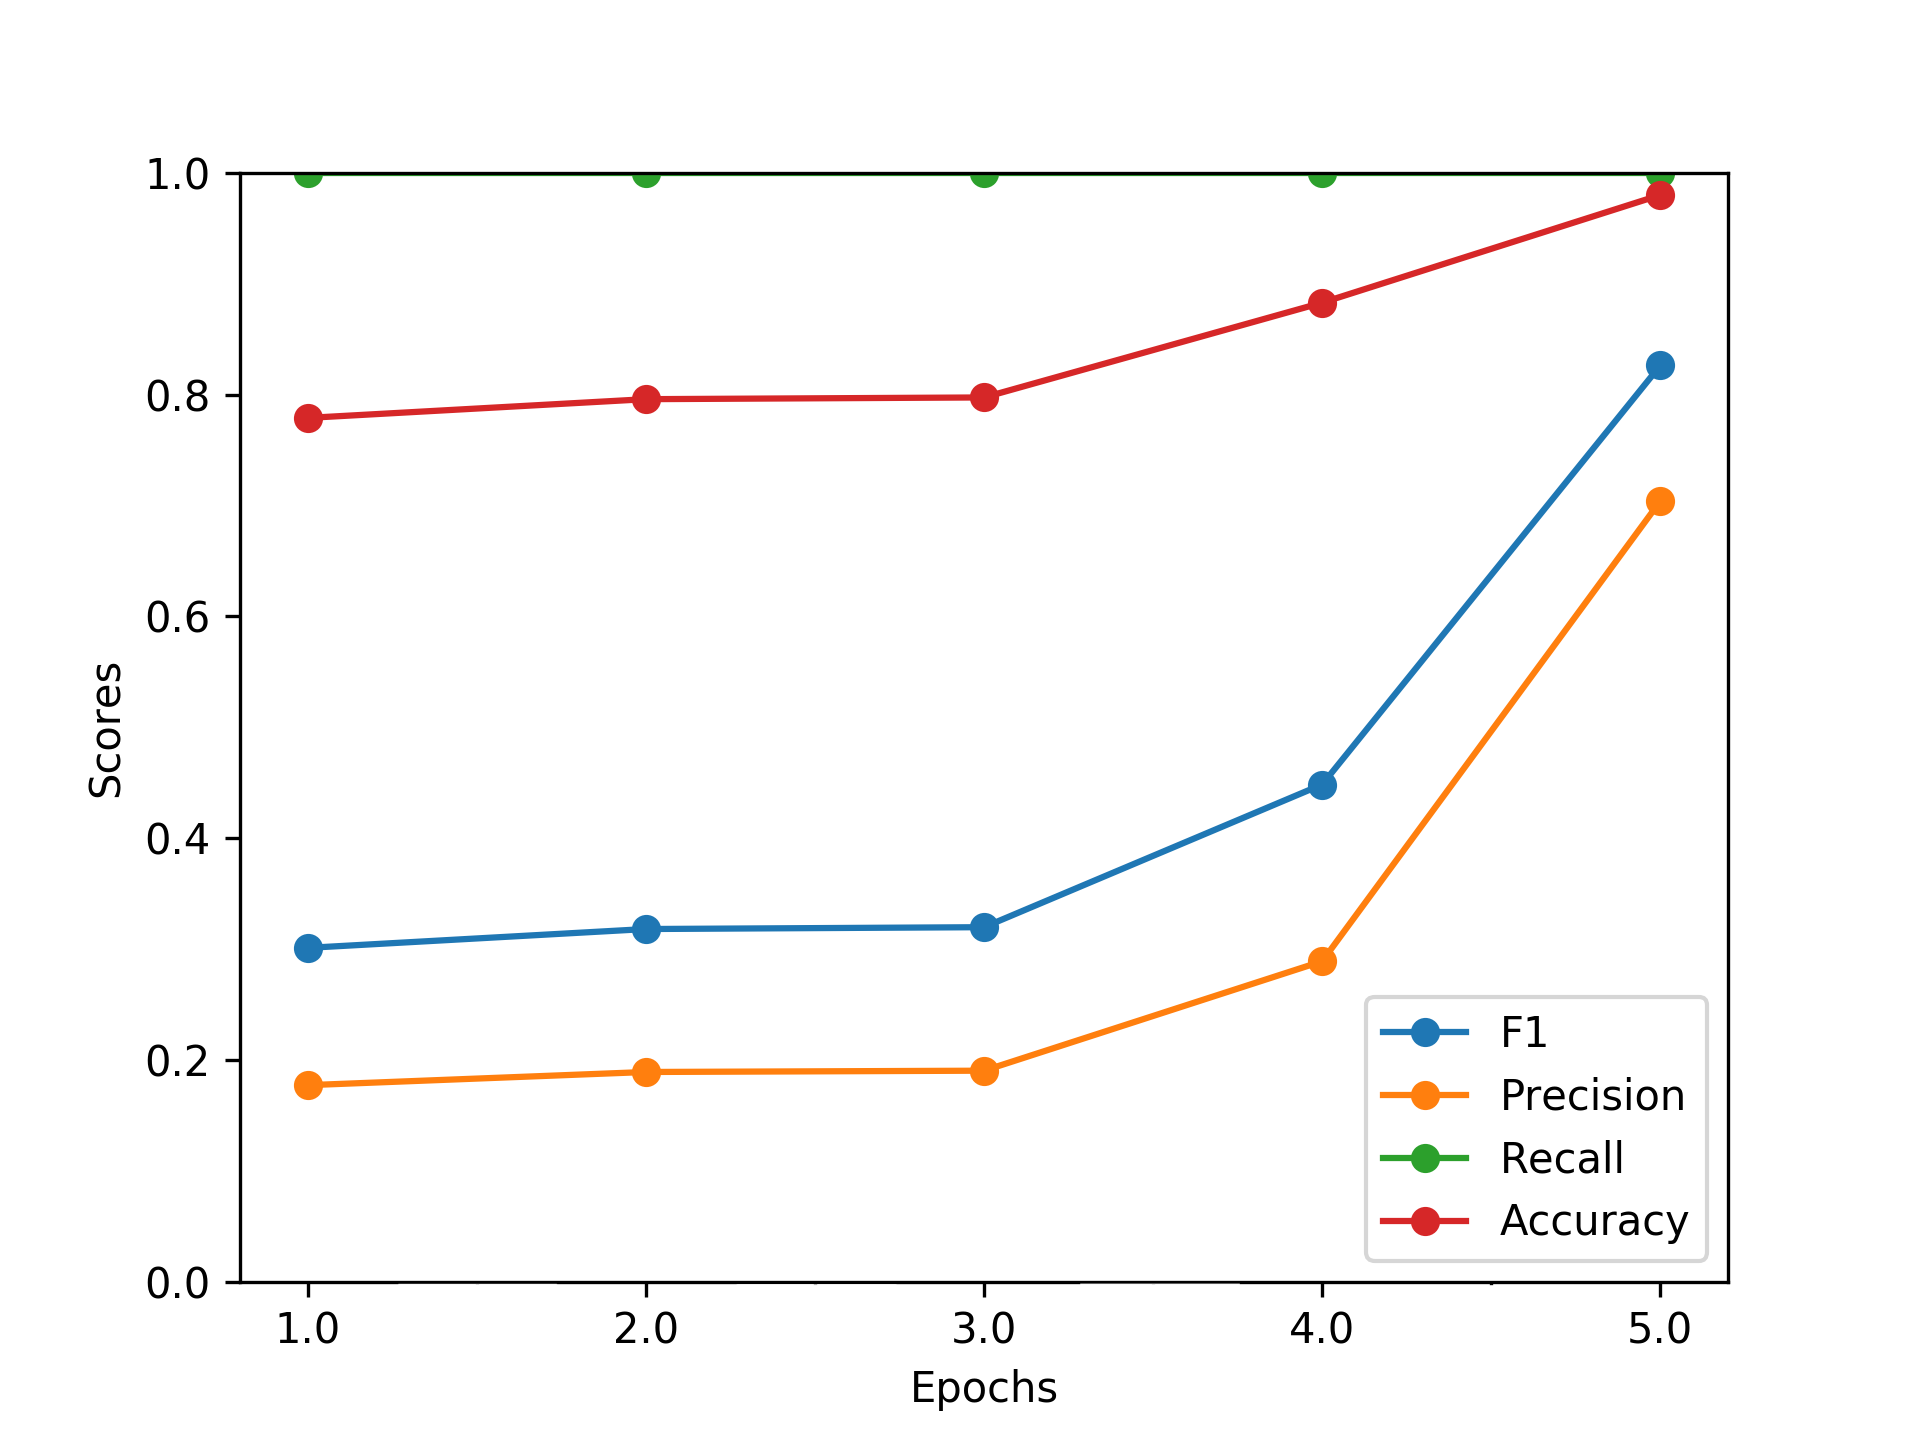
\includegraphics[width=0.322\textwidth]{results/transfer/bert_multiclass_0.15_transfer_metrics_per_epoch.png}}
\hspace{\fill}
   \subfloat[GPT-2\label{fig:results_transfer_multiclass_per_epoch_0.10} ]{%
      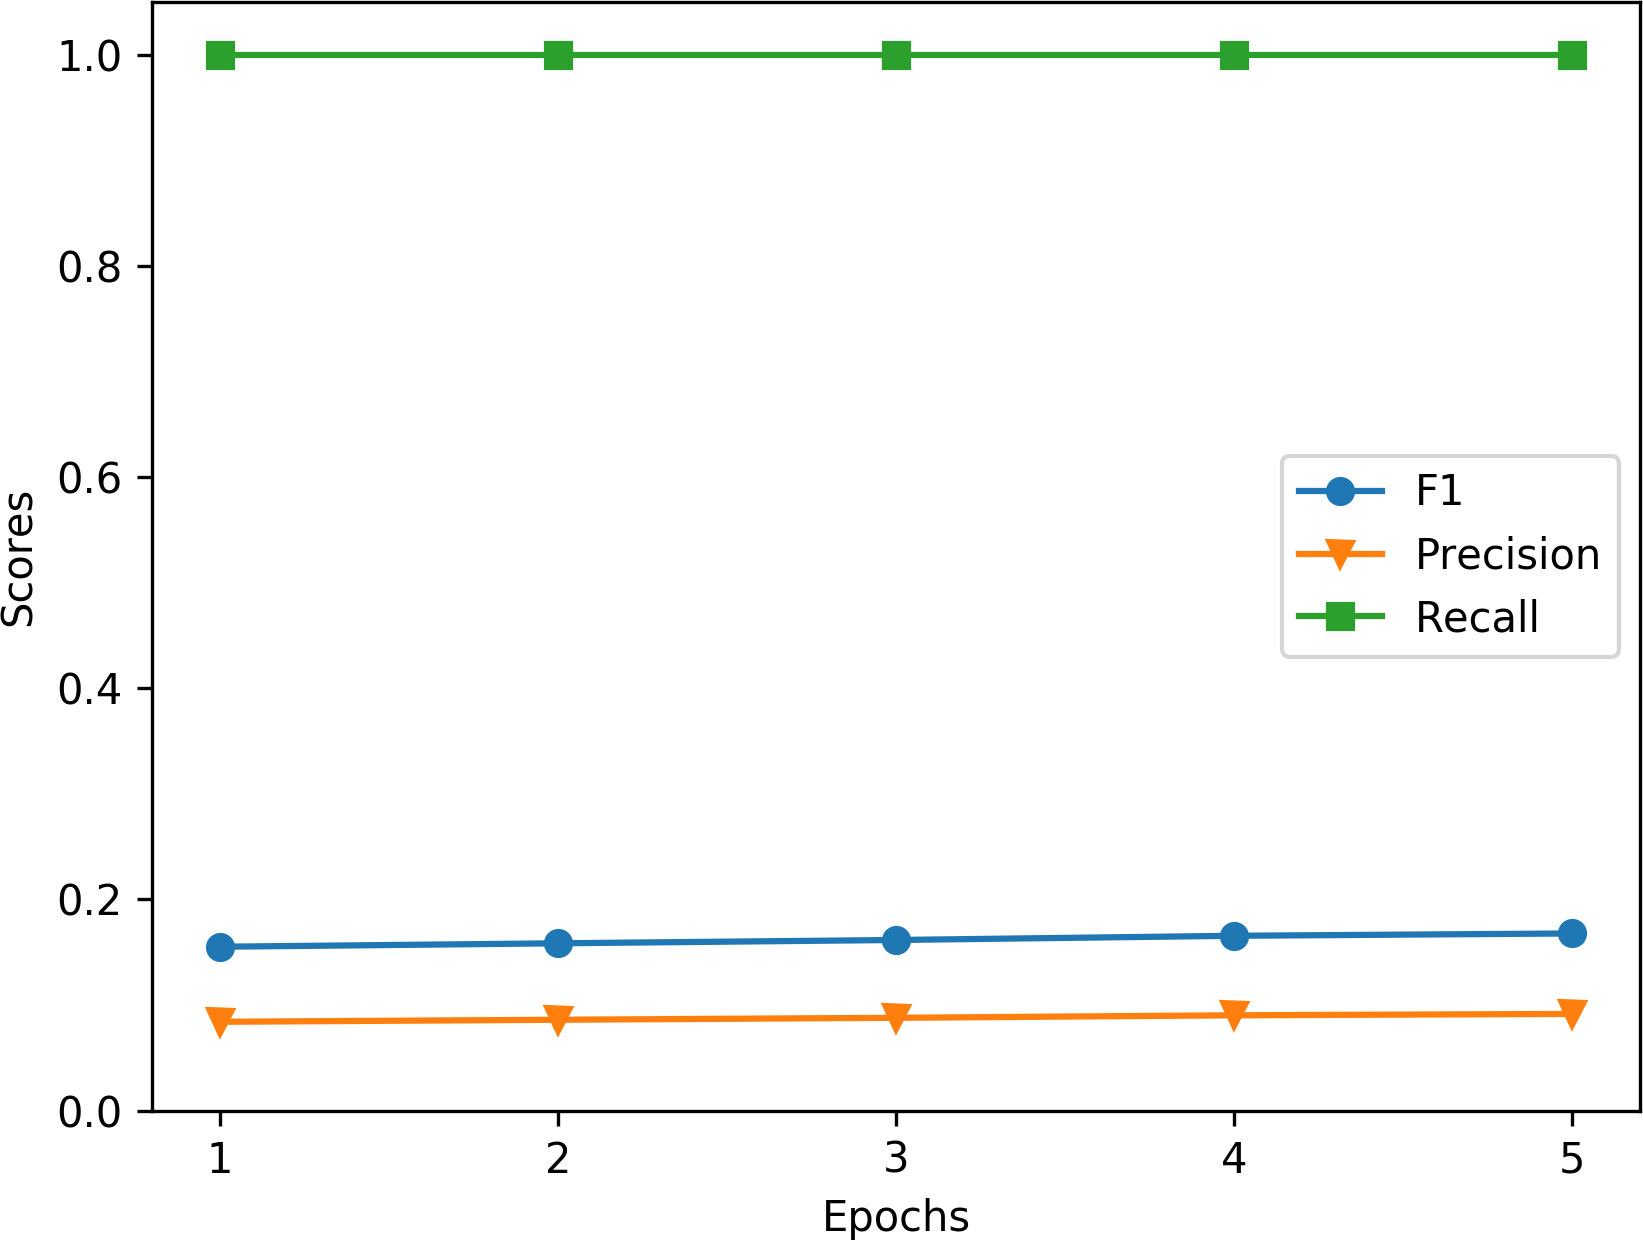
\includegraphics[width=0.322\textwidth]{results/transfer/gpt_multiclass_0.15_transfer_metrics_per_epoch.png}}
\hspace{\fill}
   \subfloat[XL\label{fig:results_transfer_multiclass_per_epoch_0.15}]{%
      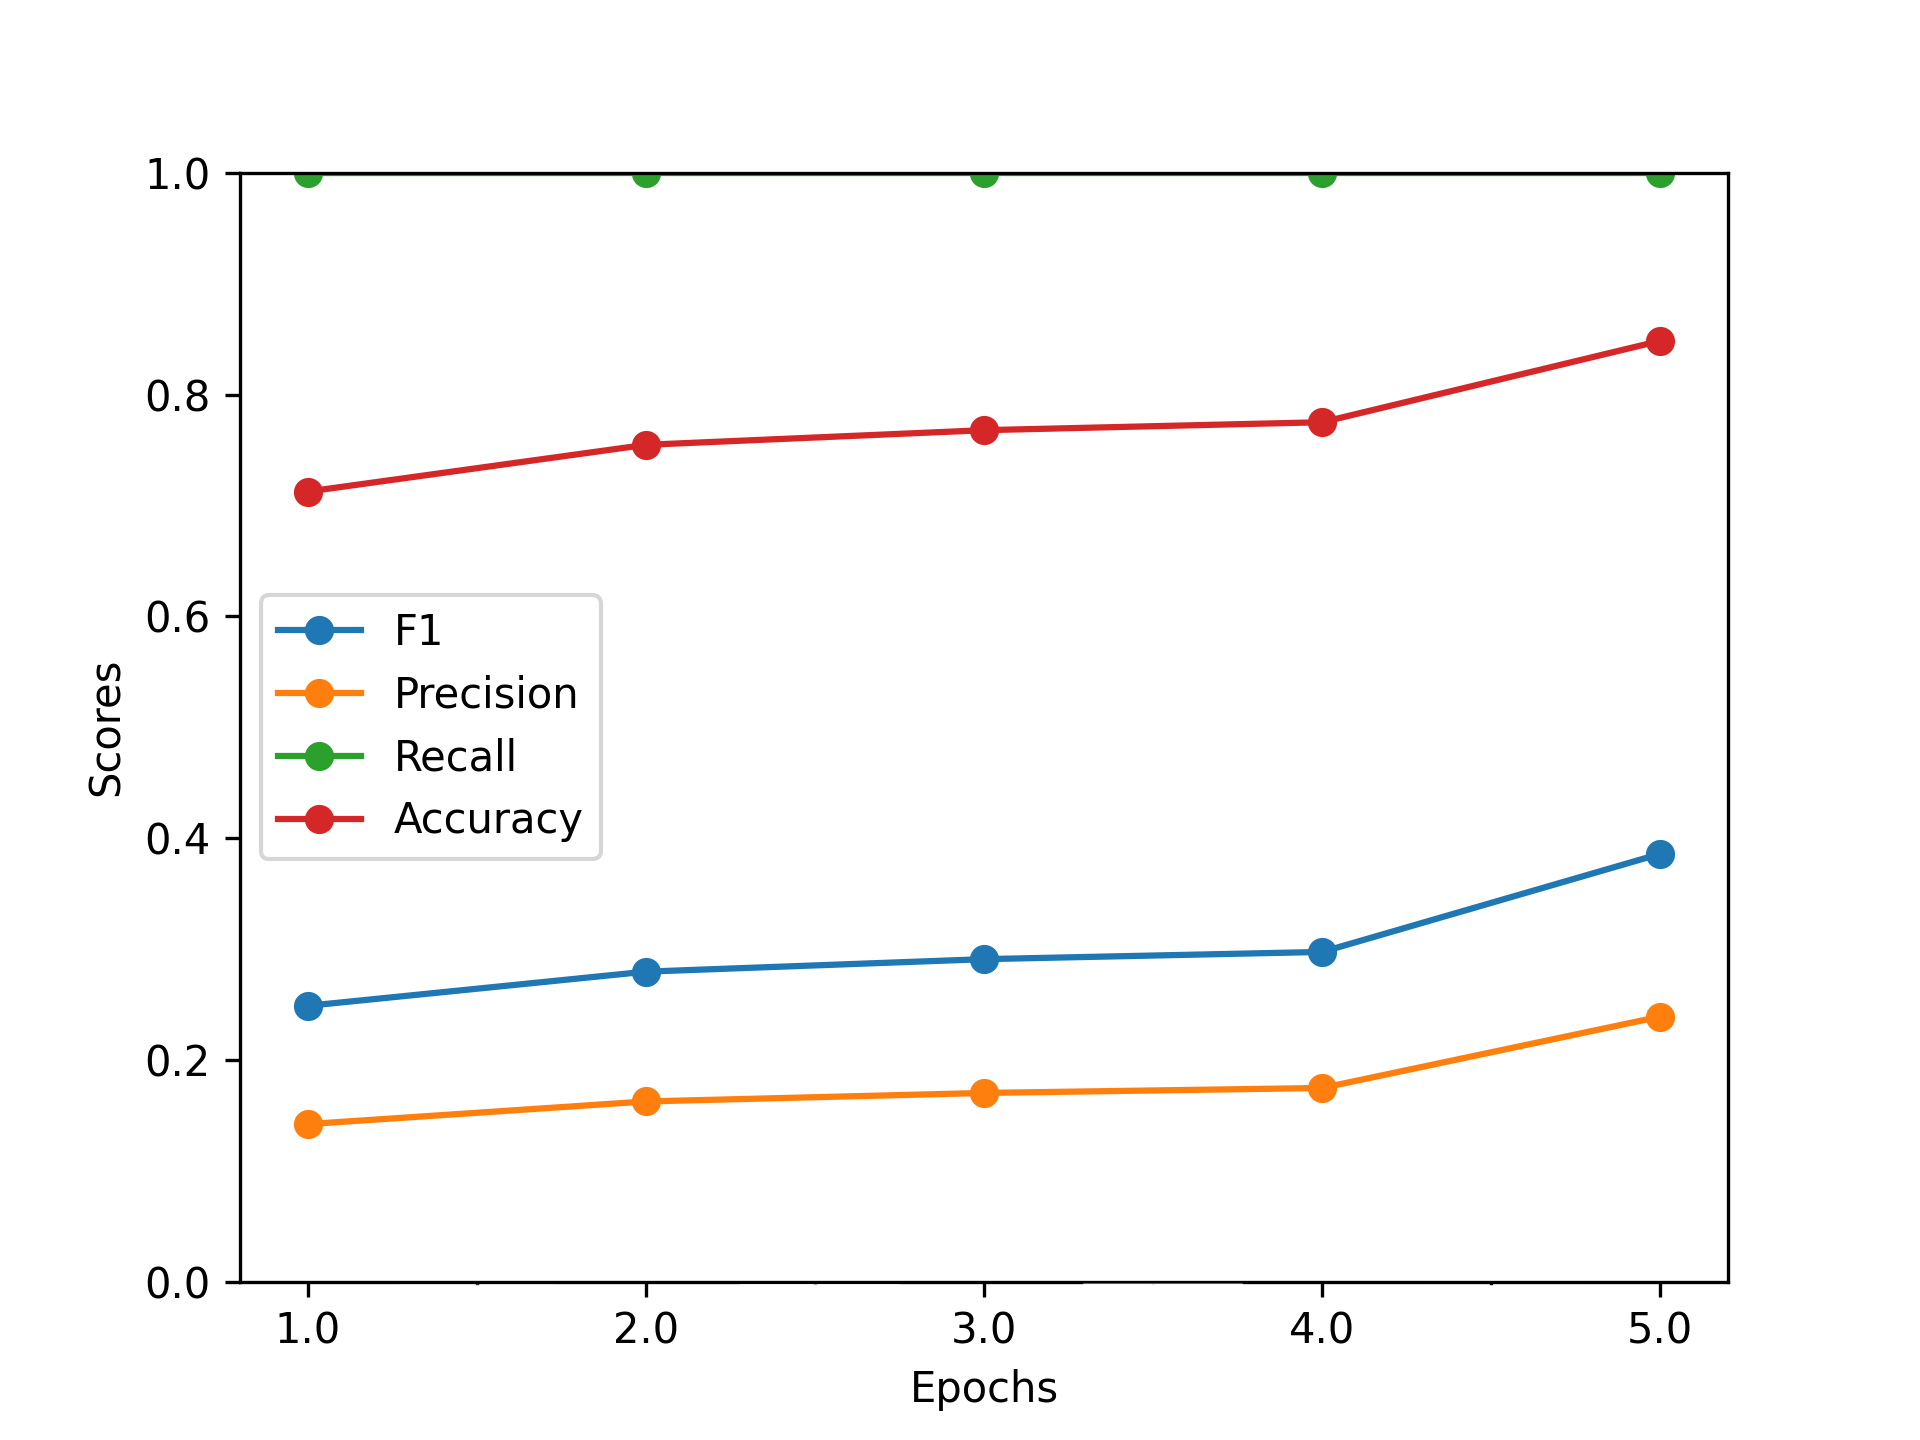
\includegraphics[width=0.322\textwidth]{results/transfer/xl_multiclass_0.15_transfer_metrics_per_epoch.png}}\\
\caption{\label{fig:results_transfer_multiclass_per_epoch}Improvement of metrics for transfer of knowledge per additional learning epoch, with 15\% alterations and injection of semantically different anomalies, using classification.}
\end{figure*}

\begin{comment}
\begin{figure*}[ht!]
   \subfloat[Bert\label{fig:roc_curve_bert_transfer_multiclass}]{%
      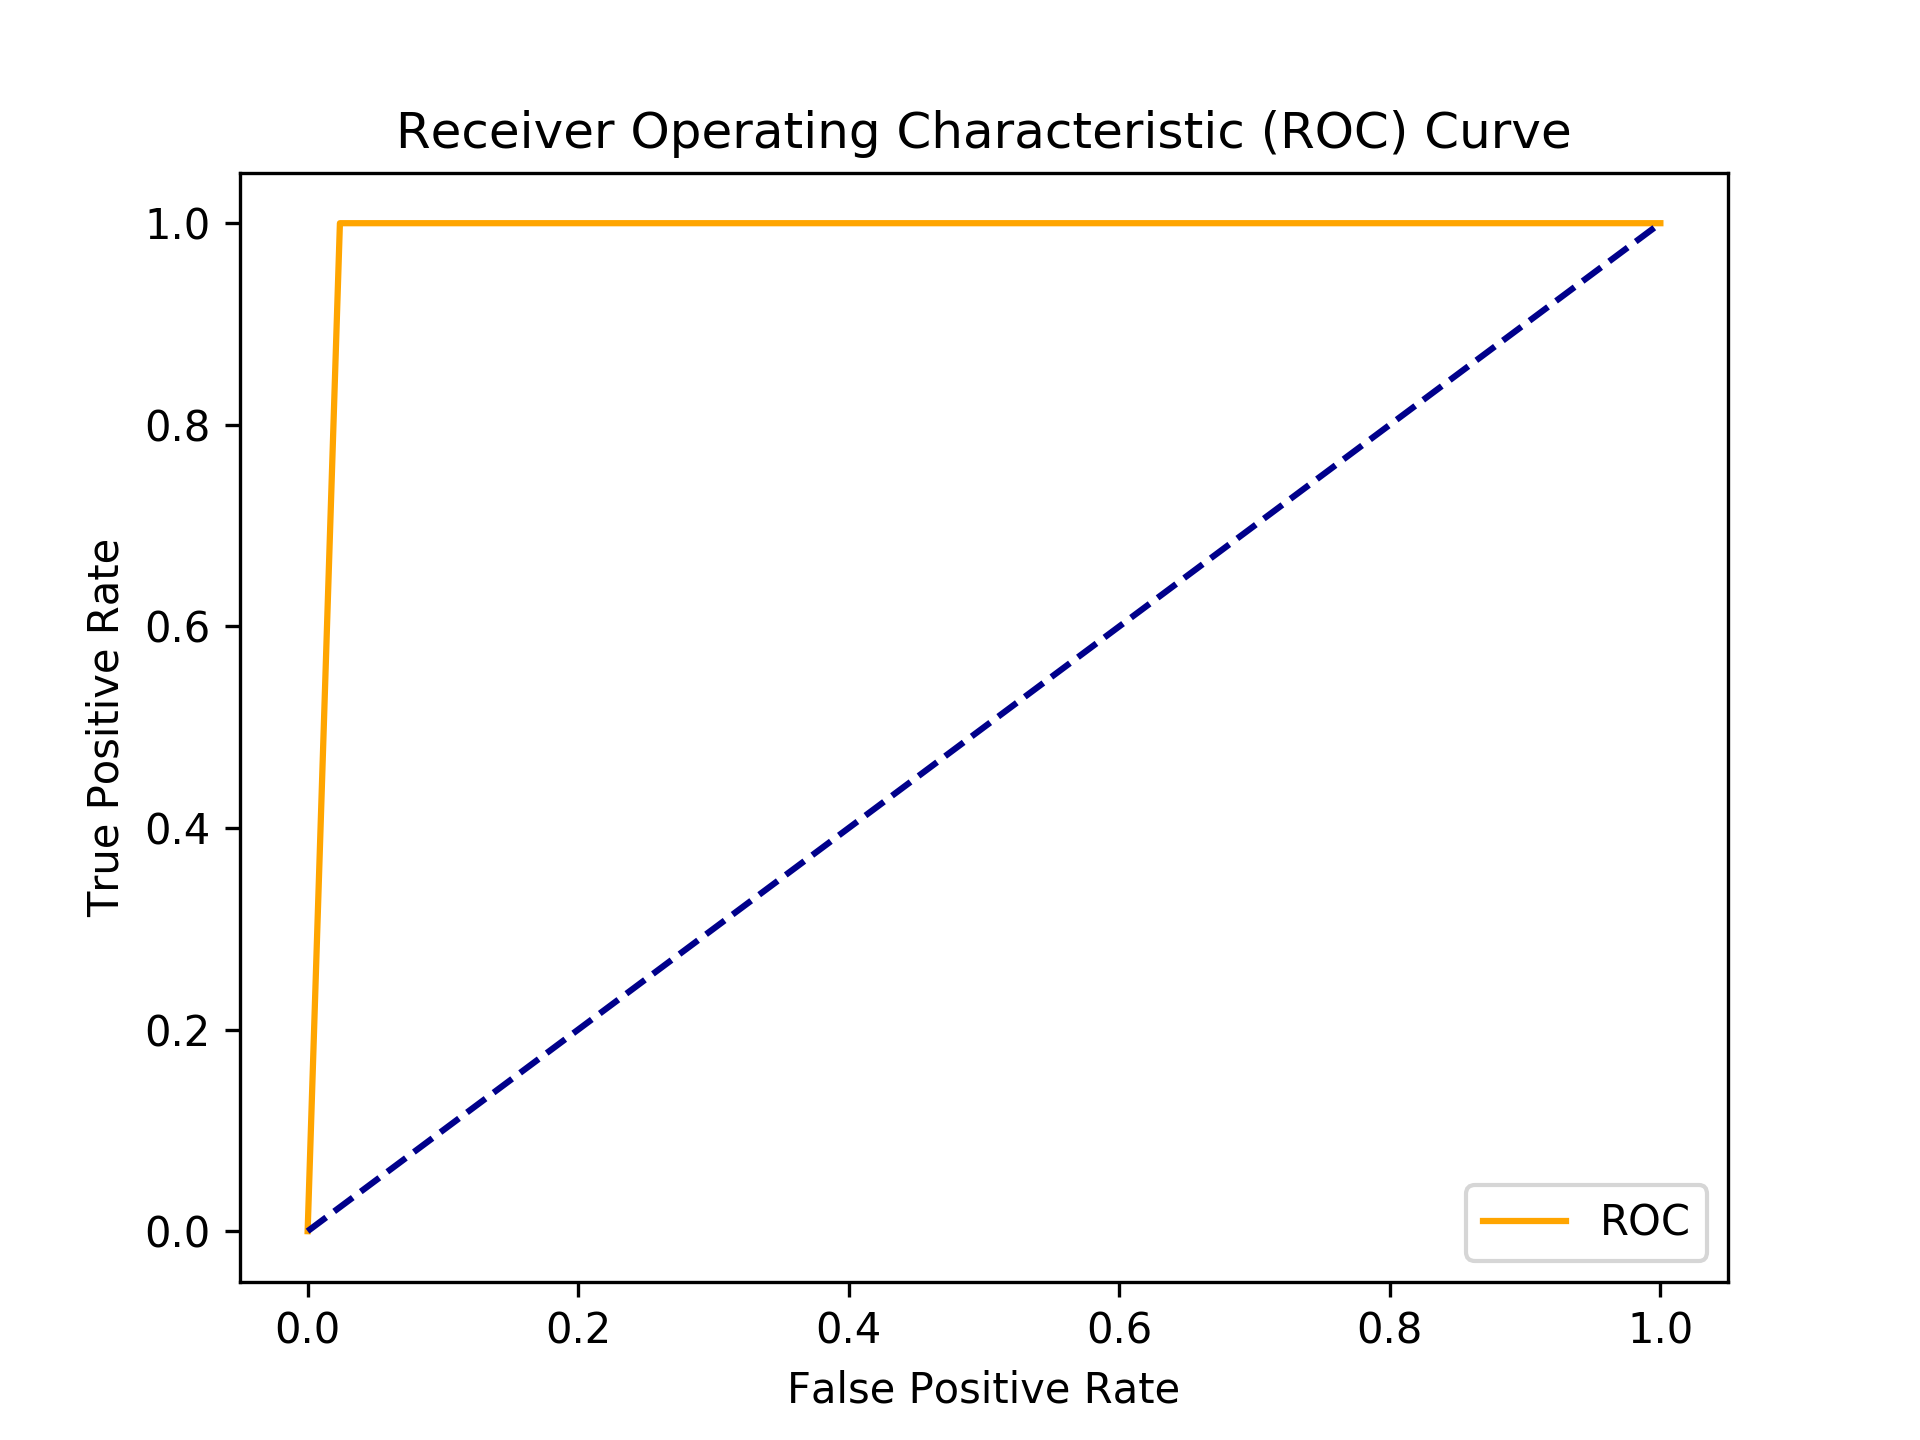
\includegraphics[trim={1cm 0.5cm 0cm 1cm}, width=0.322\textwidth]{results/transfer/roc_curve_transfer_multiclass_bert_0.15.png}}
\hspace{\fill}
   \subfloat[GPT-2\label{fig:roc_curve_gpt_transfer_multiclass} ]{%
      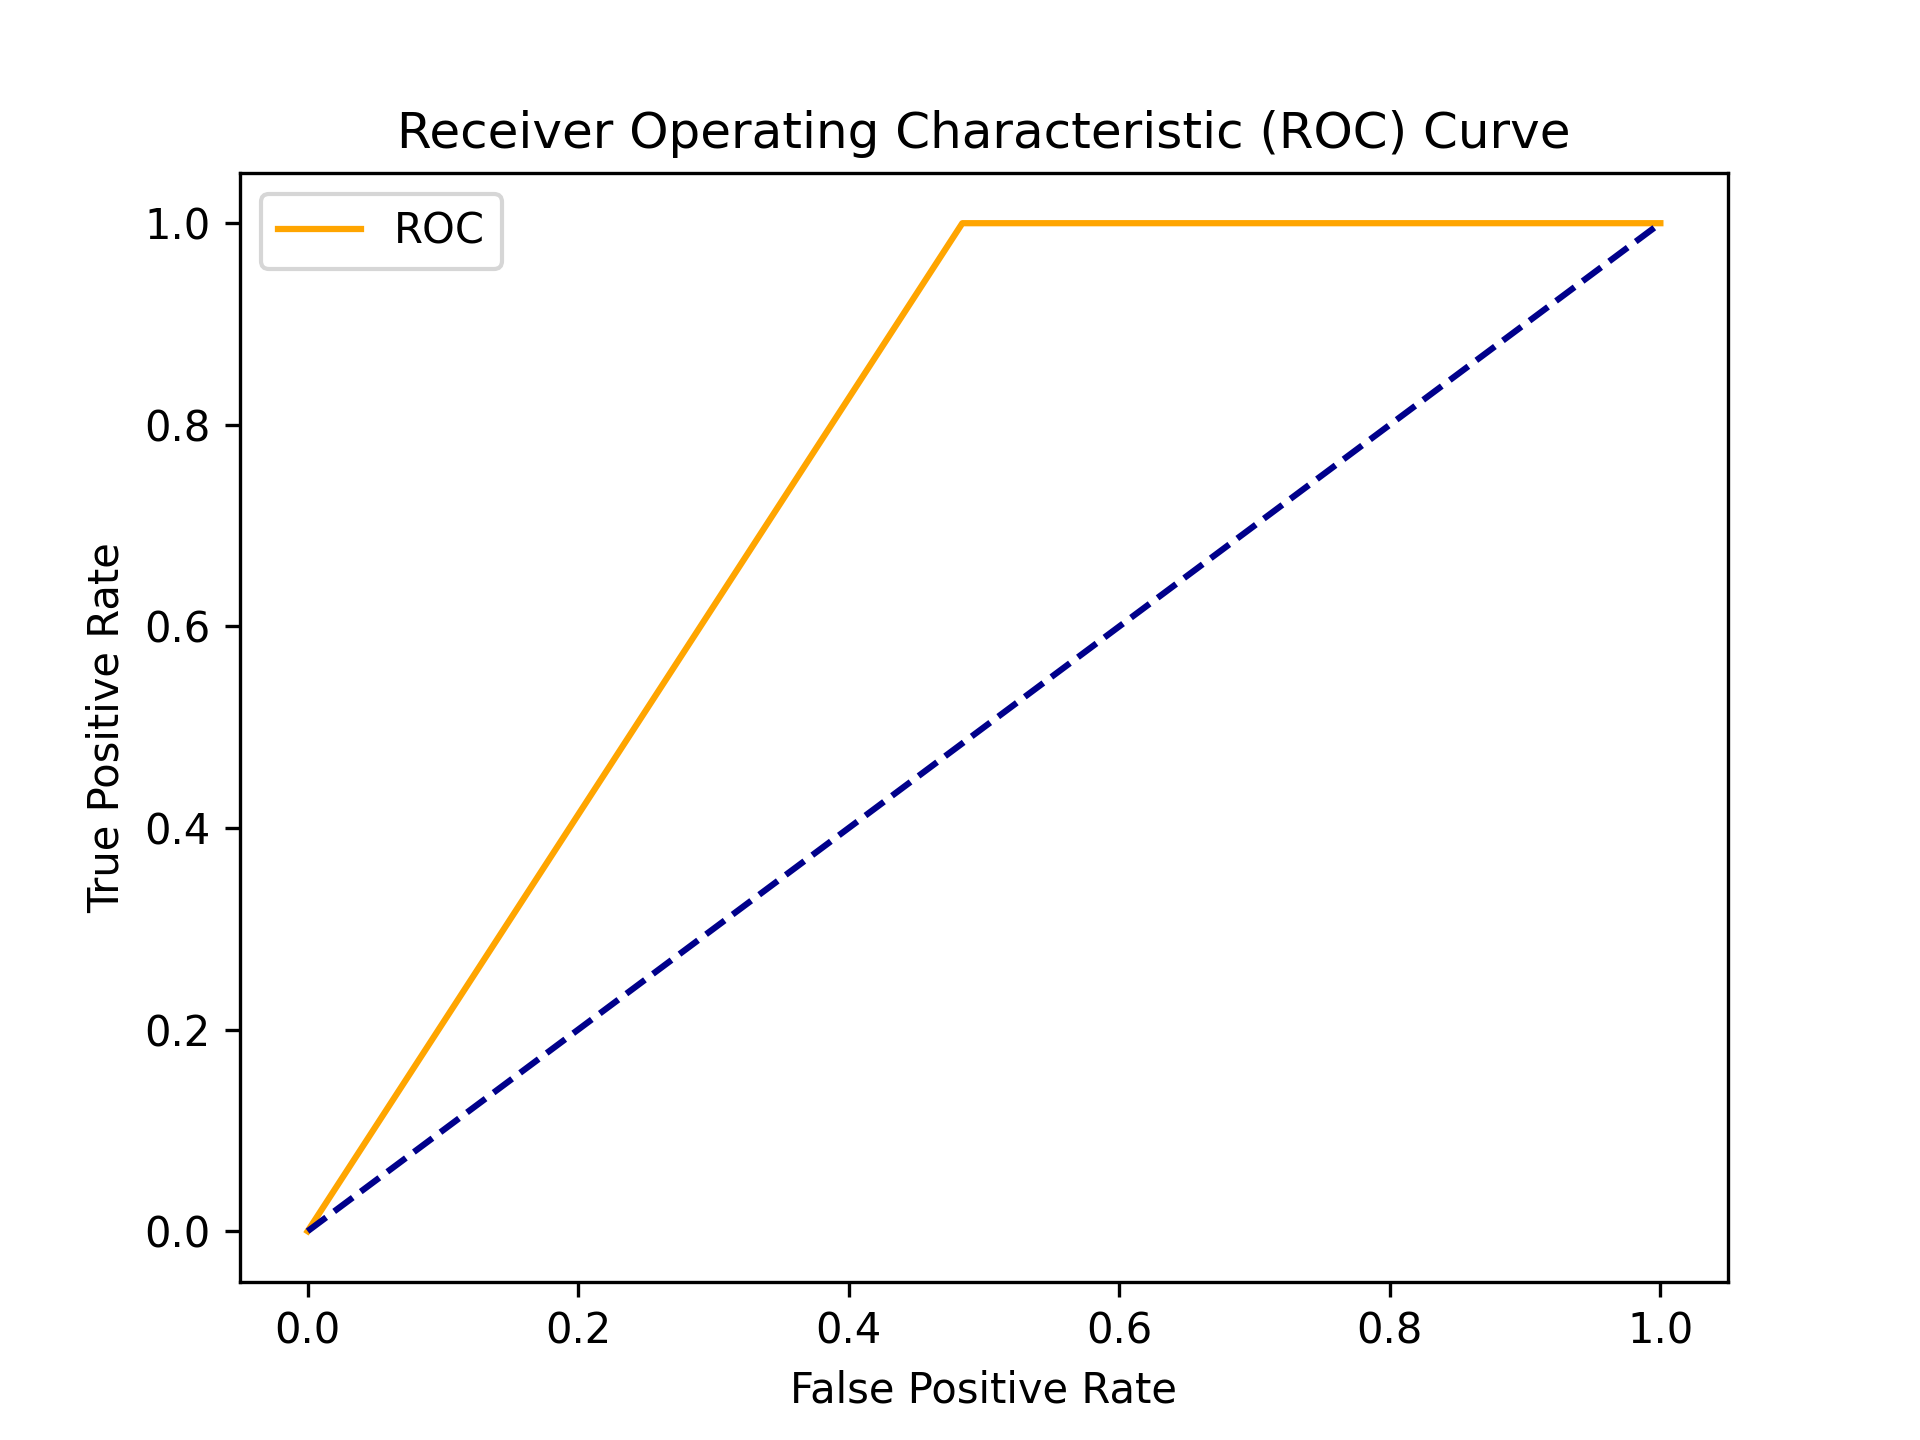
\includegraphics[trim={1cm 0.5cm 0cm 1cm}, width=0.322\textwidth]{results/transfer/roc_curve_transfer_multiclass_gpt_0.15.png}}
\hspace{\fill}
   \subfloat[XL\label{fig:roc_curve_xl_transfer_multiclass}]{%
      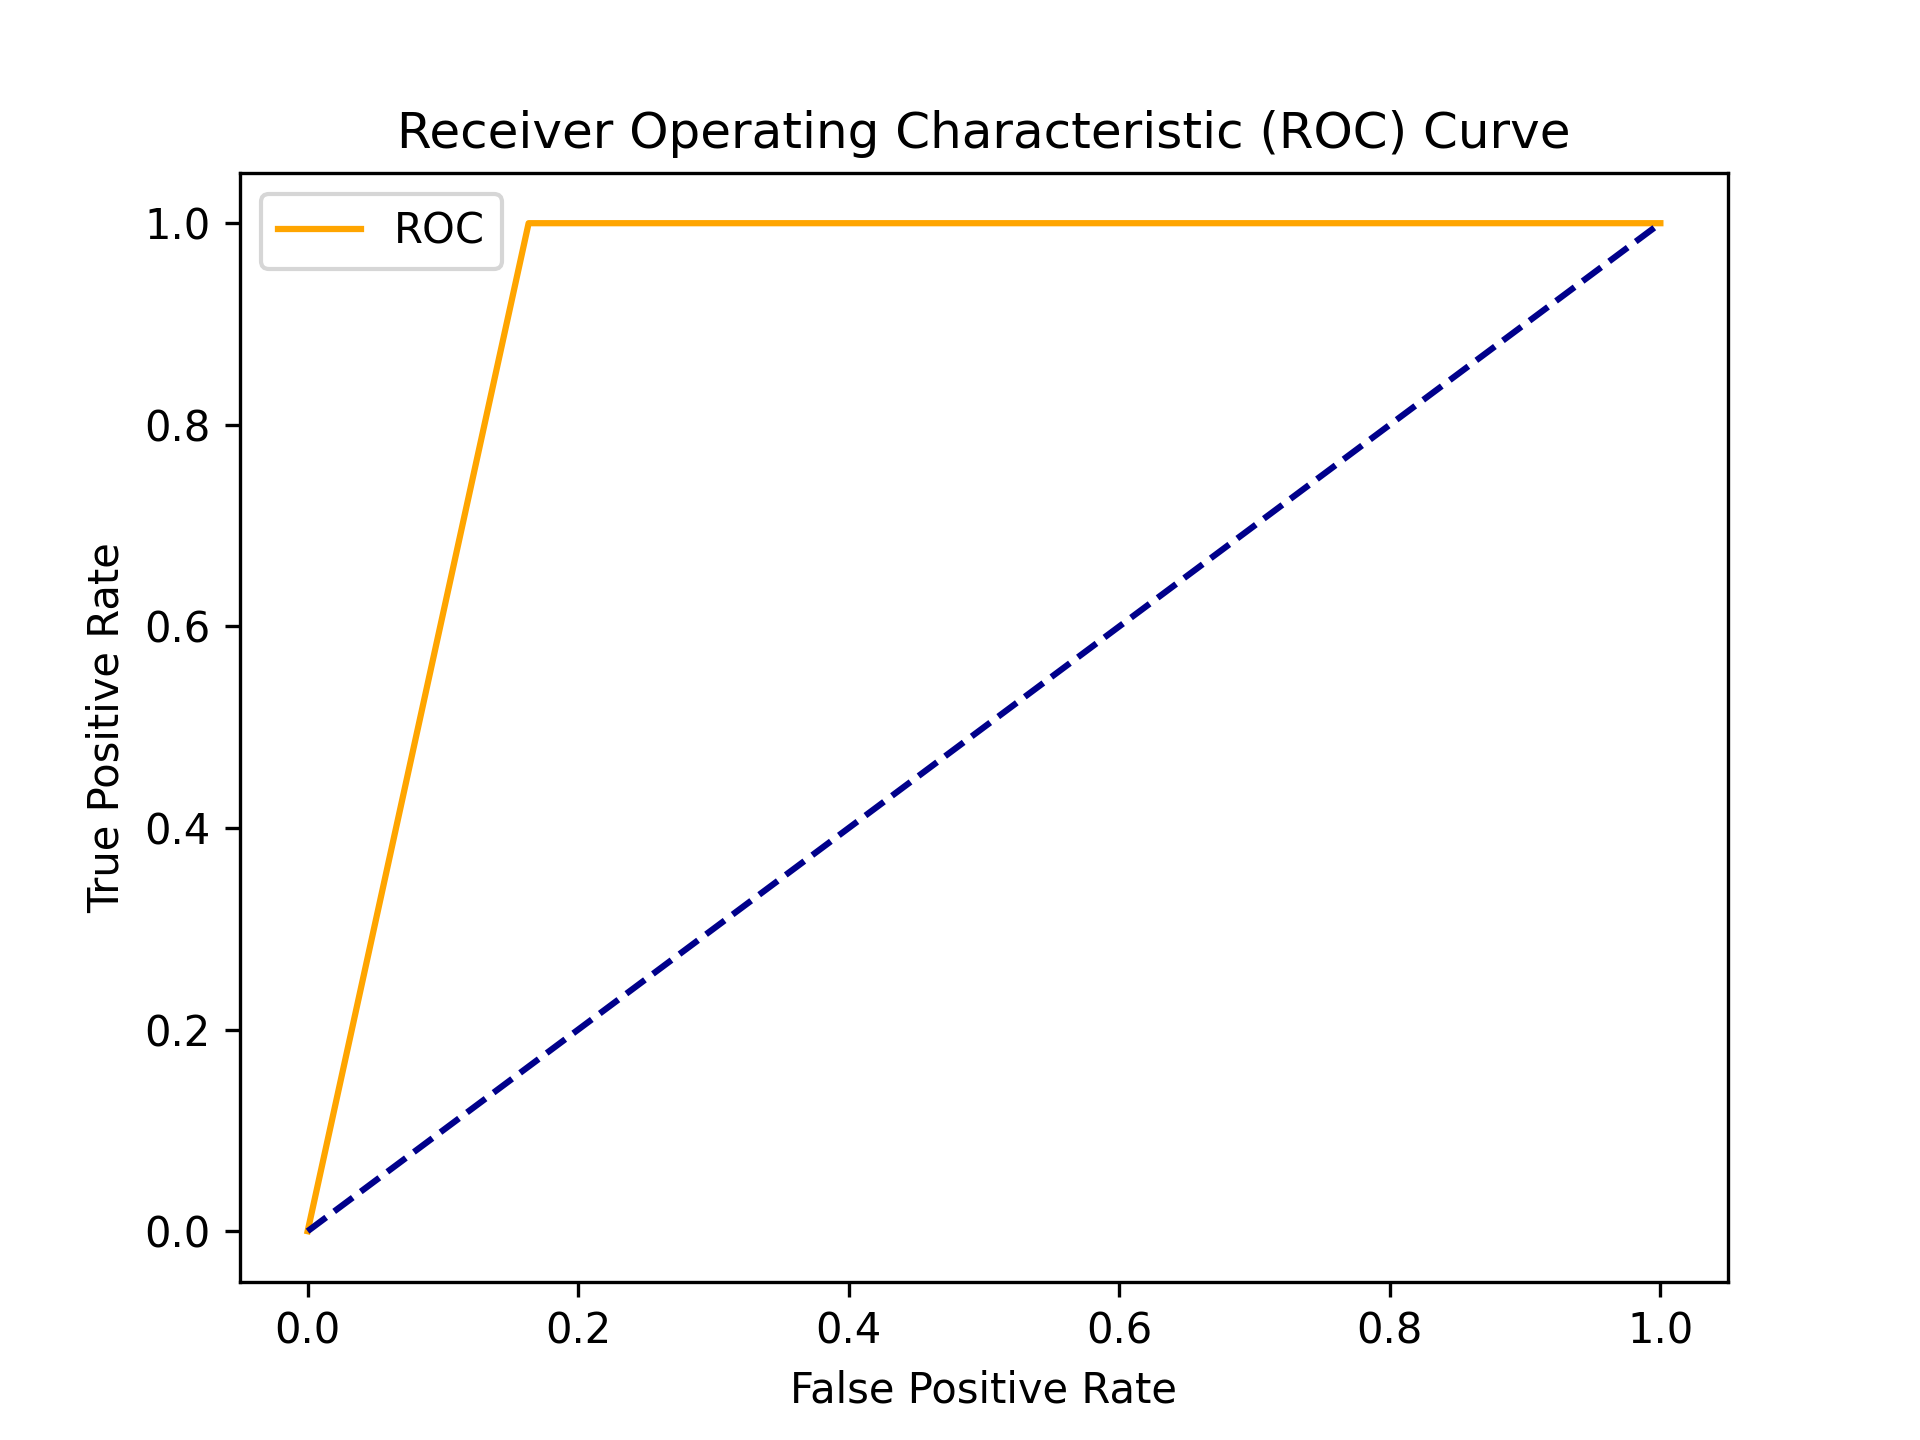
\includegraphics[trim={1cm 0.5cm 0cm 1cm}, width=0.322\textwidth]{results/transfer/roc_curve_transfer_multiclass_xl_0.15.png}}\\
\caption{\label{fig:results_transfer_multiclass_roc}ROC-Curve for transfer of knowledge using regression with 15\% alterations.}
\end{figure*}
\end{comment}

\begin{figure}[h]
  \centering
  \captionsetup{justification=centering}
  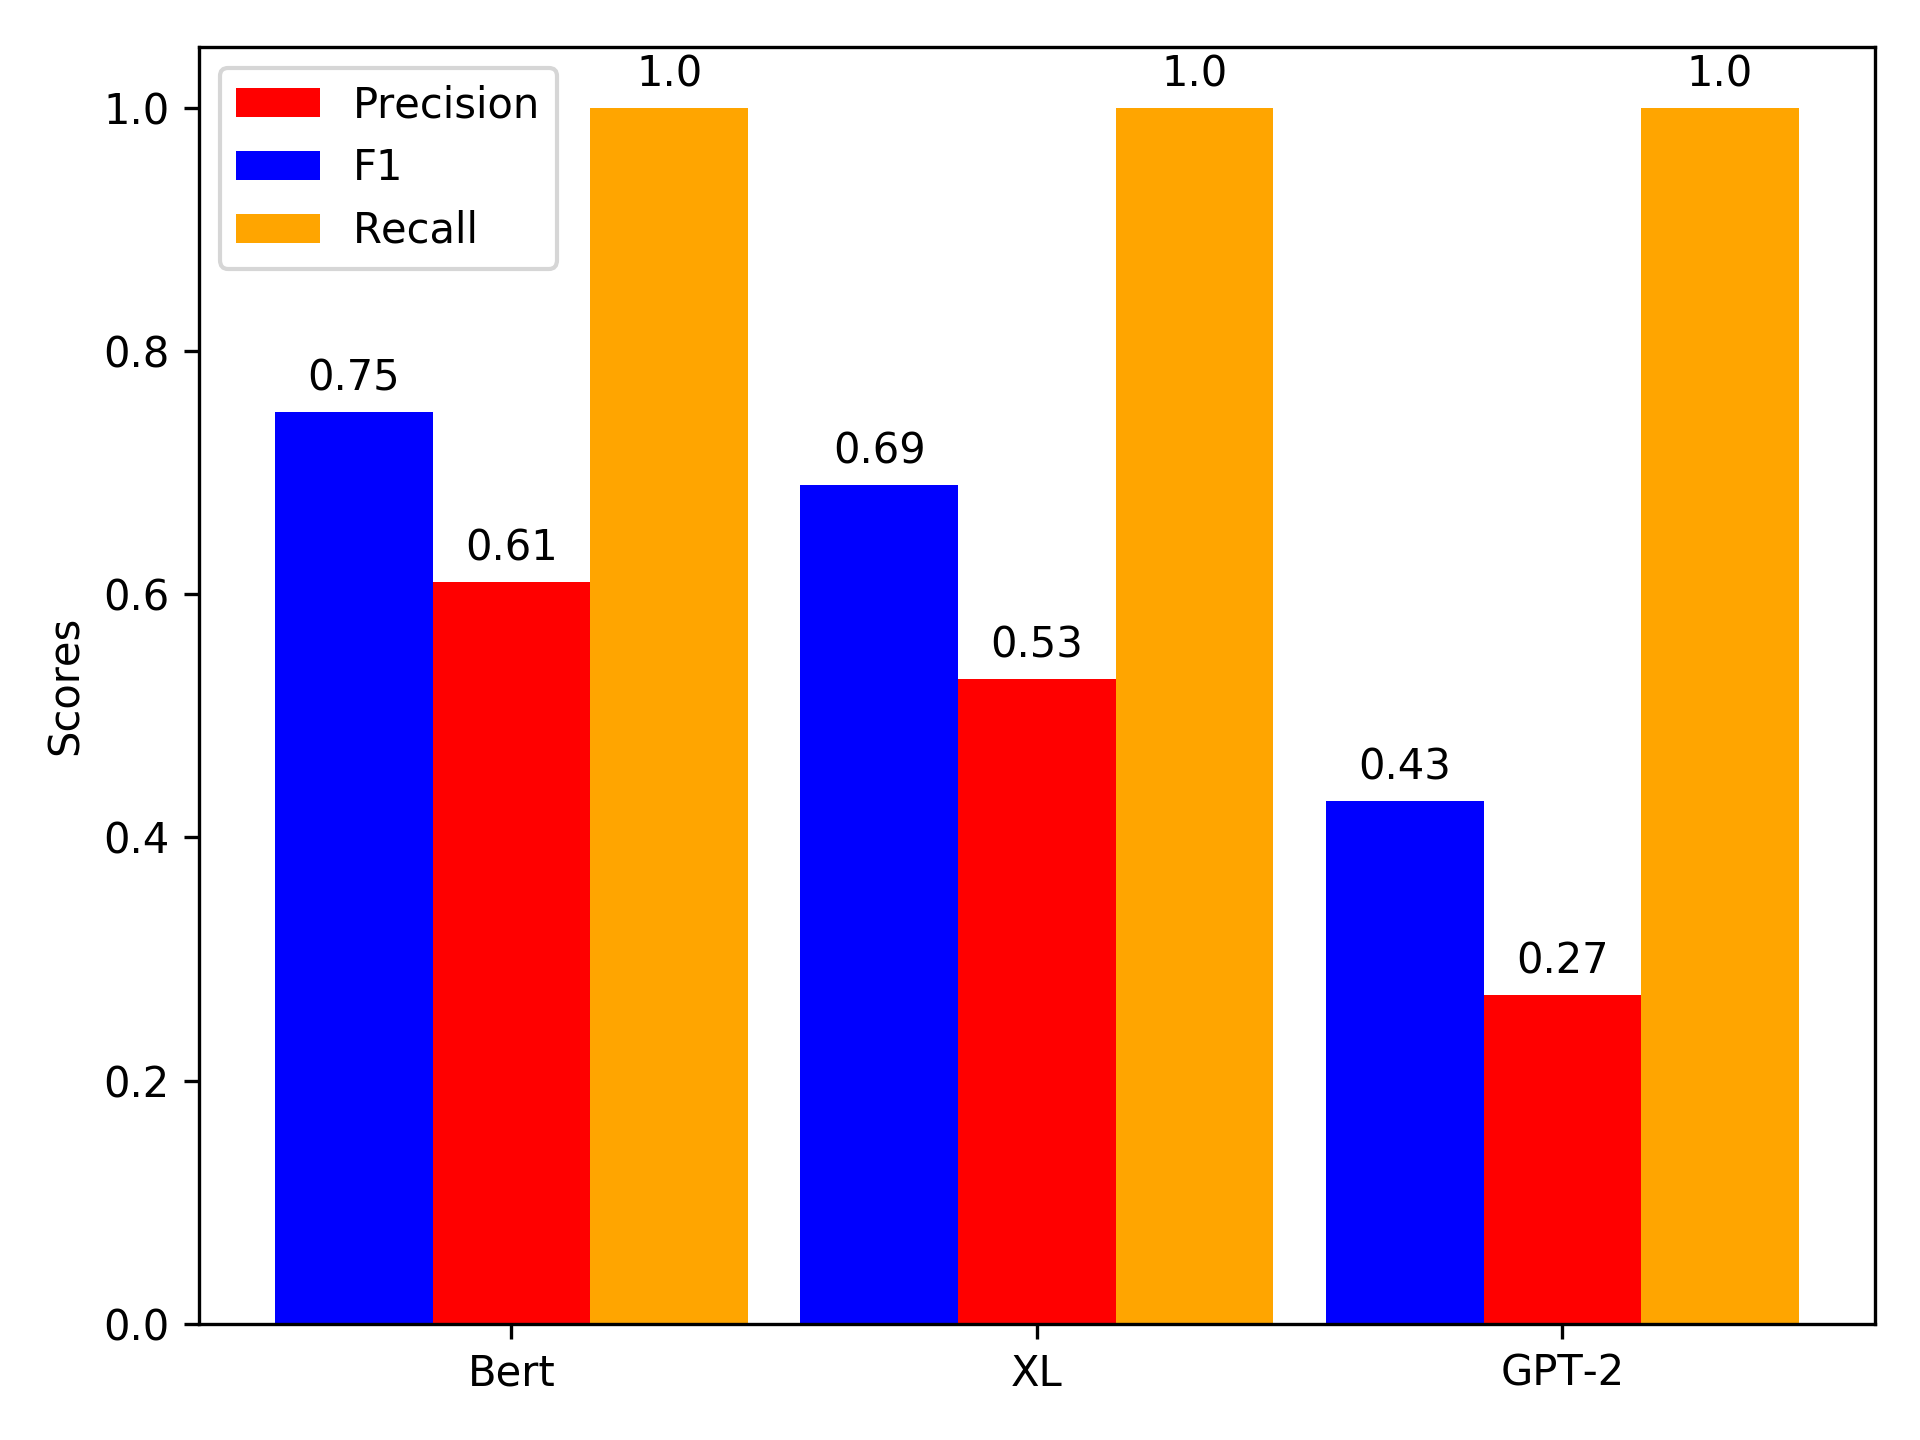
\includegraphics[width=8cm]{results/transfer_multiclass_replace_half.png}\\
  \caption{Transfer of knowledge. 15\% alteration, injection of semantically similar anomalies, using regression.}
  \label{fig:replace_words_classification_transfer}
\end{figure}

\clearpage
\section{Discussion of Results\label{sec:discussion_results}}
By evaluating three different language models, it has been shown that the used word embeddings can highly influence the quality of the results for anomaly detection, with different word embeddings having strengths and weaknesses in different categories.

While GPT-2 shows strengths in the regression-based approach with injection of semantically different anomalies -- achieving a F1-score of up to 0.94, and being  far better overall than Bert and XL-Transformers -- it shows clear disadvantages when semantically similar anomalies are injected, where Bert is the best of the three language models, with a F1-score of 0.71. GPT-2 shows very stable results also for the transfer of knowledge approach, using regression for injection of semantically different anomalies, with a F1-score of  up to 0.97, while Bert and XL-Transformers degrade substantially when the ratio of alteration is increased. Yet again GPT-2 drops significantly for the injection of semantically similar anomalies, with a F1-score of 0.08, while Bert is achieving the best results with a F1-score of 0.63.

For the classification-based approach, the results show a different picture in general. While both Bert and XL-Transformers are able to achieve a recall score of 1.0 for injection of semantically different and similar anomalies, GPT-2only achieves around 0.7. The results do not differ as substantially for GPT-2 between semantically different (F1-score up to 0.43 for 15\% alterations) and semantically similar injections (F1-score of 0.71) as they do in comparison to the regression-based approach. Bert is able to achieve an F1-score of up to 0.67  for 15\% alterations and injection of semantically different anomalies, XL-Transformers reaches up to 0.53. For semantically similar anomalies, Bert achieves a F1-score of 0.94 and XL-Transformers 0.81. Bert is clearly ahead in this category.
For the transfer of knowledge using classification, and injection of a semantically different anomaly, all are able to achieve full recall scores, due to the semantic nature of the anomaly. Bert is clearly the best in this category. Also for the semantically similar injection, Bert is the most fit language model.

Overall it can be stated that Bert shows the most steady and best results overall, while GPT-2 is highly dependent on the semantic nature of the injected anomaly, showing very good results for the injection of semantically different anomalies, and very unreliable results for the injection of semantically similar anomalies using the regression approach. XL-Transformers, on the other hand, profits from the regression-based approach.

The results prove the usability of the presented model. All three language models are generally suitable for anomaly detection.
%For anomaly detection on one dataset using the regression approach, GPT-2 shows strong results, with F1-Scores of 0.95 when altering 5\% of log sequences, and 0.93 when altering the log lines, the quality of the results don't degrade much, when alteration ratios are increased, where Bert and XL-Transformers show decreases of 0.1 to 0.2 percentage points when increasing the alteration ratio from 5\% to 15\%. Yet, when the log events are completely reversed, GPT-2 achieves an F1-Score of only 0.55, where Bert and XL achieve 0.98, almost perfectly detecting the wrong sequence of log events.


%For the regression-based approach on one dataset and injection of semantically different anomalies, GPT-2 beats Bert and XL-Transformers clearly with regards to all metrics, achieving an F1-score of 0.94 and recall of 1.0, for injecting alterations on 15\% of the sequences of logs, where Bert achieves 0.56 F1-score and recall of 1.0 and XL-Transformers only achieves 0.31 F1-score and 0.64 recall. Similar results can be seen for the alterations of log lines, where Bert and XL-Transformers improve by around 10 percentage points, while GPT-2 degrades by around 8 percentage points.

%For the injection of semantically similar anomalies using the regression-based approach, GPT-2 shows a completely different picture, with a F1-score of 0.09, precision of 0.13 and recall of 0.07, while Bert and XL-Transformers show improved results for all metrics. This shows that for the regression-based approach, the quality of the embeddings produced by GPT-2 does not suffice in order to differentiate between normal log lines and highly manipulated log lines.

%Using the classification-based approach on one dataset and injection of semantically different anomalies, GPT-2 shows weaker results than Bert and XL-Transformers as it does for the same anomalies using the regression-based approach, with Bert being ahead of XL-Transformers and GPT-2 in all categories. For injecting alterations on 15\% of the sequences of logs Bert returns a F1-score of 0.54 and recall of 1.0, XL-Transformers returns a F1-score of 0.41 and recall of 1.0, and GPT-2 returns a F1-score of 0.36 and recall of 0.7. For altering of log events, the F1-score of Bert is 13 percentage points better, for XL-Transformers it is 12 percentage points better, and for GPT only 7 percentage points better, while recall stays unchanged for all.

%For the injection of semantically similar anomalies using the classification-based approach, we see that all language models show improved overall metrics, especially with regards to F1-score.

%For the transfer of knowledge approach, the results show a different picture. Using the regression approach and injection of semantically different anomalies, GPT-2 is still ahead of the other two, returning a F1-score of 0.97 and recall of 1.0, while Bert achieves a F1-score of 0.68 and recall of 1.0, and finally XL-Transformers delivering again the least promising results of all three with a F1-score of 0.26 and recall of 0.47 for 15\% alteration ratio. 

%Again, as in prediction on one dataset, for injection of semantically similar anomalies in the transfer of knowledge approach using regression, we see that GPT-2 shows significant weaknesses in all metrics, returning a F1-score of only 0.08 and recall of 0.05, while Bert achieves a F1-score of 0.63 and recall of 0.7 and XL-Transformers achieving a F1-score of 0.55 and recall of also 0.7.

%On the other hand, for transfer of knowledge using the classification-based approach, for 15\% alterations and injection of semantically different anomalies, GPT-2 shows results that are not very promising, while still being able to find all anomalies, but showing a small F1-Score of only 0.17, where Bert is able to reach a F1-Score of 0.81 and XL-Transformers achieving 0.38. It is also visible, that GPT-2 seems to not profit as much from the few-shot learning on the new training dataset, where the metrics stay almost the same throughout between epochs 1 and 5, yet Bert shows improvements from an F1-Score of 0.3 to 0.8 between epoch 1 and 5.

%For transfer of knowledge using the classification approach, 15\% alterations and injection of semantically similar anomalies, especially XL-Transformers and GPT-2 show much better results than for the injection of semantically different anomalies.

%It can be summarised that Bert is the best of the three language models for classification for both types of anomaly injections and regression with semantically similar anomaly injections, while GPT-2 is the best language model for the regression-based approach with semantically different injections.

%It is evident, that with more hyperparameter-tuning, far better results can be accomplished, especially with XL-Transformers, since it obviously requires a different setup of hidden units and layers within the LSTM to achieve optimal results, however, since the model is a prototype and is supposed to show the possibility of comparing different word embeddings, not all potentials were fully tapped.

%TODO box plots of loss values in 